\documentclass{article}
\usepackage[left=2cm, right=2cm, top=1cm]{geometry}
\usepackage[utf8]{inputenc}
\usepackage{amsmath}
\usepackage{enumitem}
\usepackage{float}

\title{Radiometry Study Sheet Midterm - Final}
\author{Hannah Gallagher}
\date{October 10th, 2024}

\usepackage{natbib}
\usepackage{graphicx}

\begin{document}

\maketitle

\section{Introduction}

%Convolution 
%Eigenvalues Eigenvectors 
%Discrete fourier transform 
%Continuous transform 
%Vector basis 
%Circulant matrix
%Euler relation



% Hot keys to remember: command / on a mac comments highlighted code in and out.
Nugget the snowman wishes you good luck on your exam!

\begin{figure}[h!]
\centering
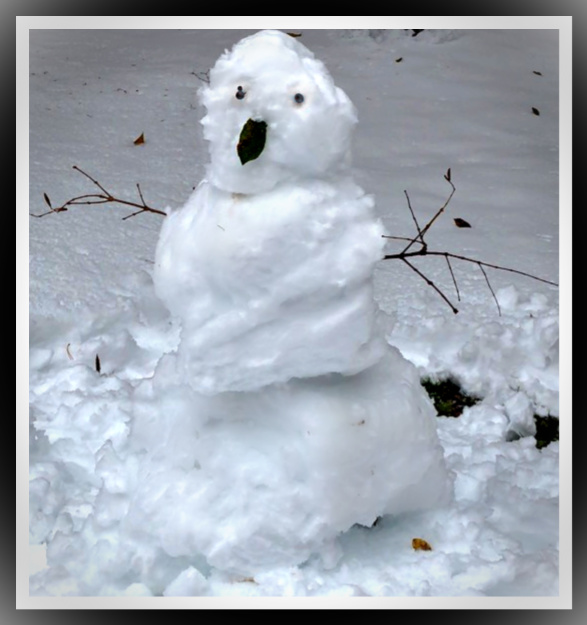
\includegraphics[scale=1]{Nugget.jpg}
\caption{Nugget the Snowman}
\label{fig:Nugget}
\end{figure}

\section{What to Focus on Final Exam}
\begin{itemize}
    \item Radiometric Definitions
    \item Extended Sources
    \item Lambertian 
    \item Isotropic 
    \item NASA Question Parameterizing Surface Integral
    \item Reflectance
    \item Fresnel Equations 
    \item Emittance 
    \item Quadrature
    \item Shot Noise 
    \item Camera Equation 
    \item Optical Depth 
    \item Noise Equivalent Power 
    \item DO NOT MESS UP RELATION OF QE to Se or whatever
    
\end{itemize}

\section{What to Focus on}

\clearpage
\subsection{NASA Question from First Homework}

\begin{figure}[h!]
\centering
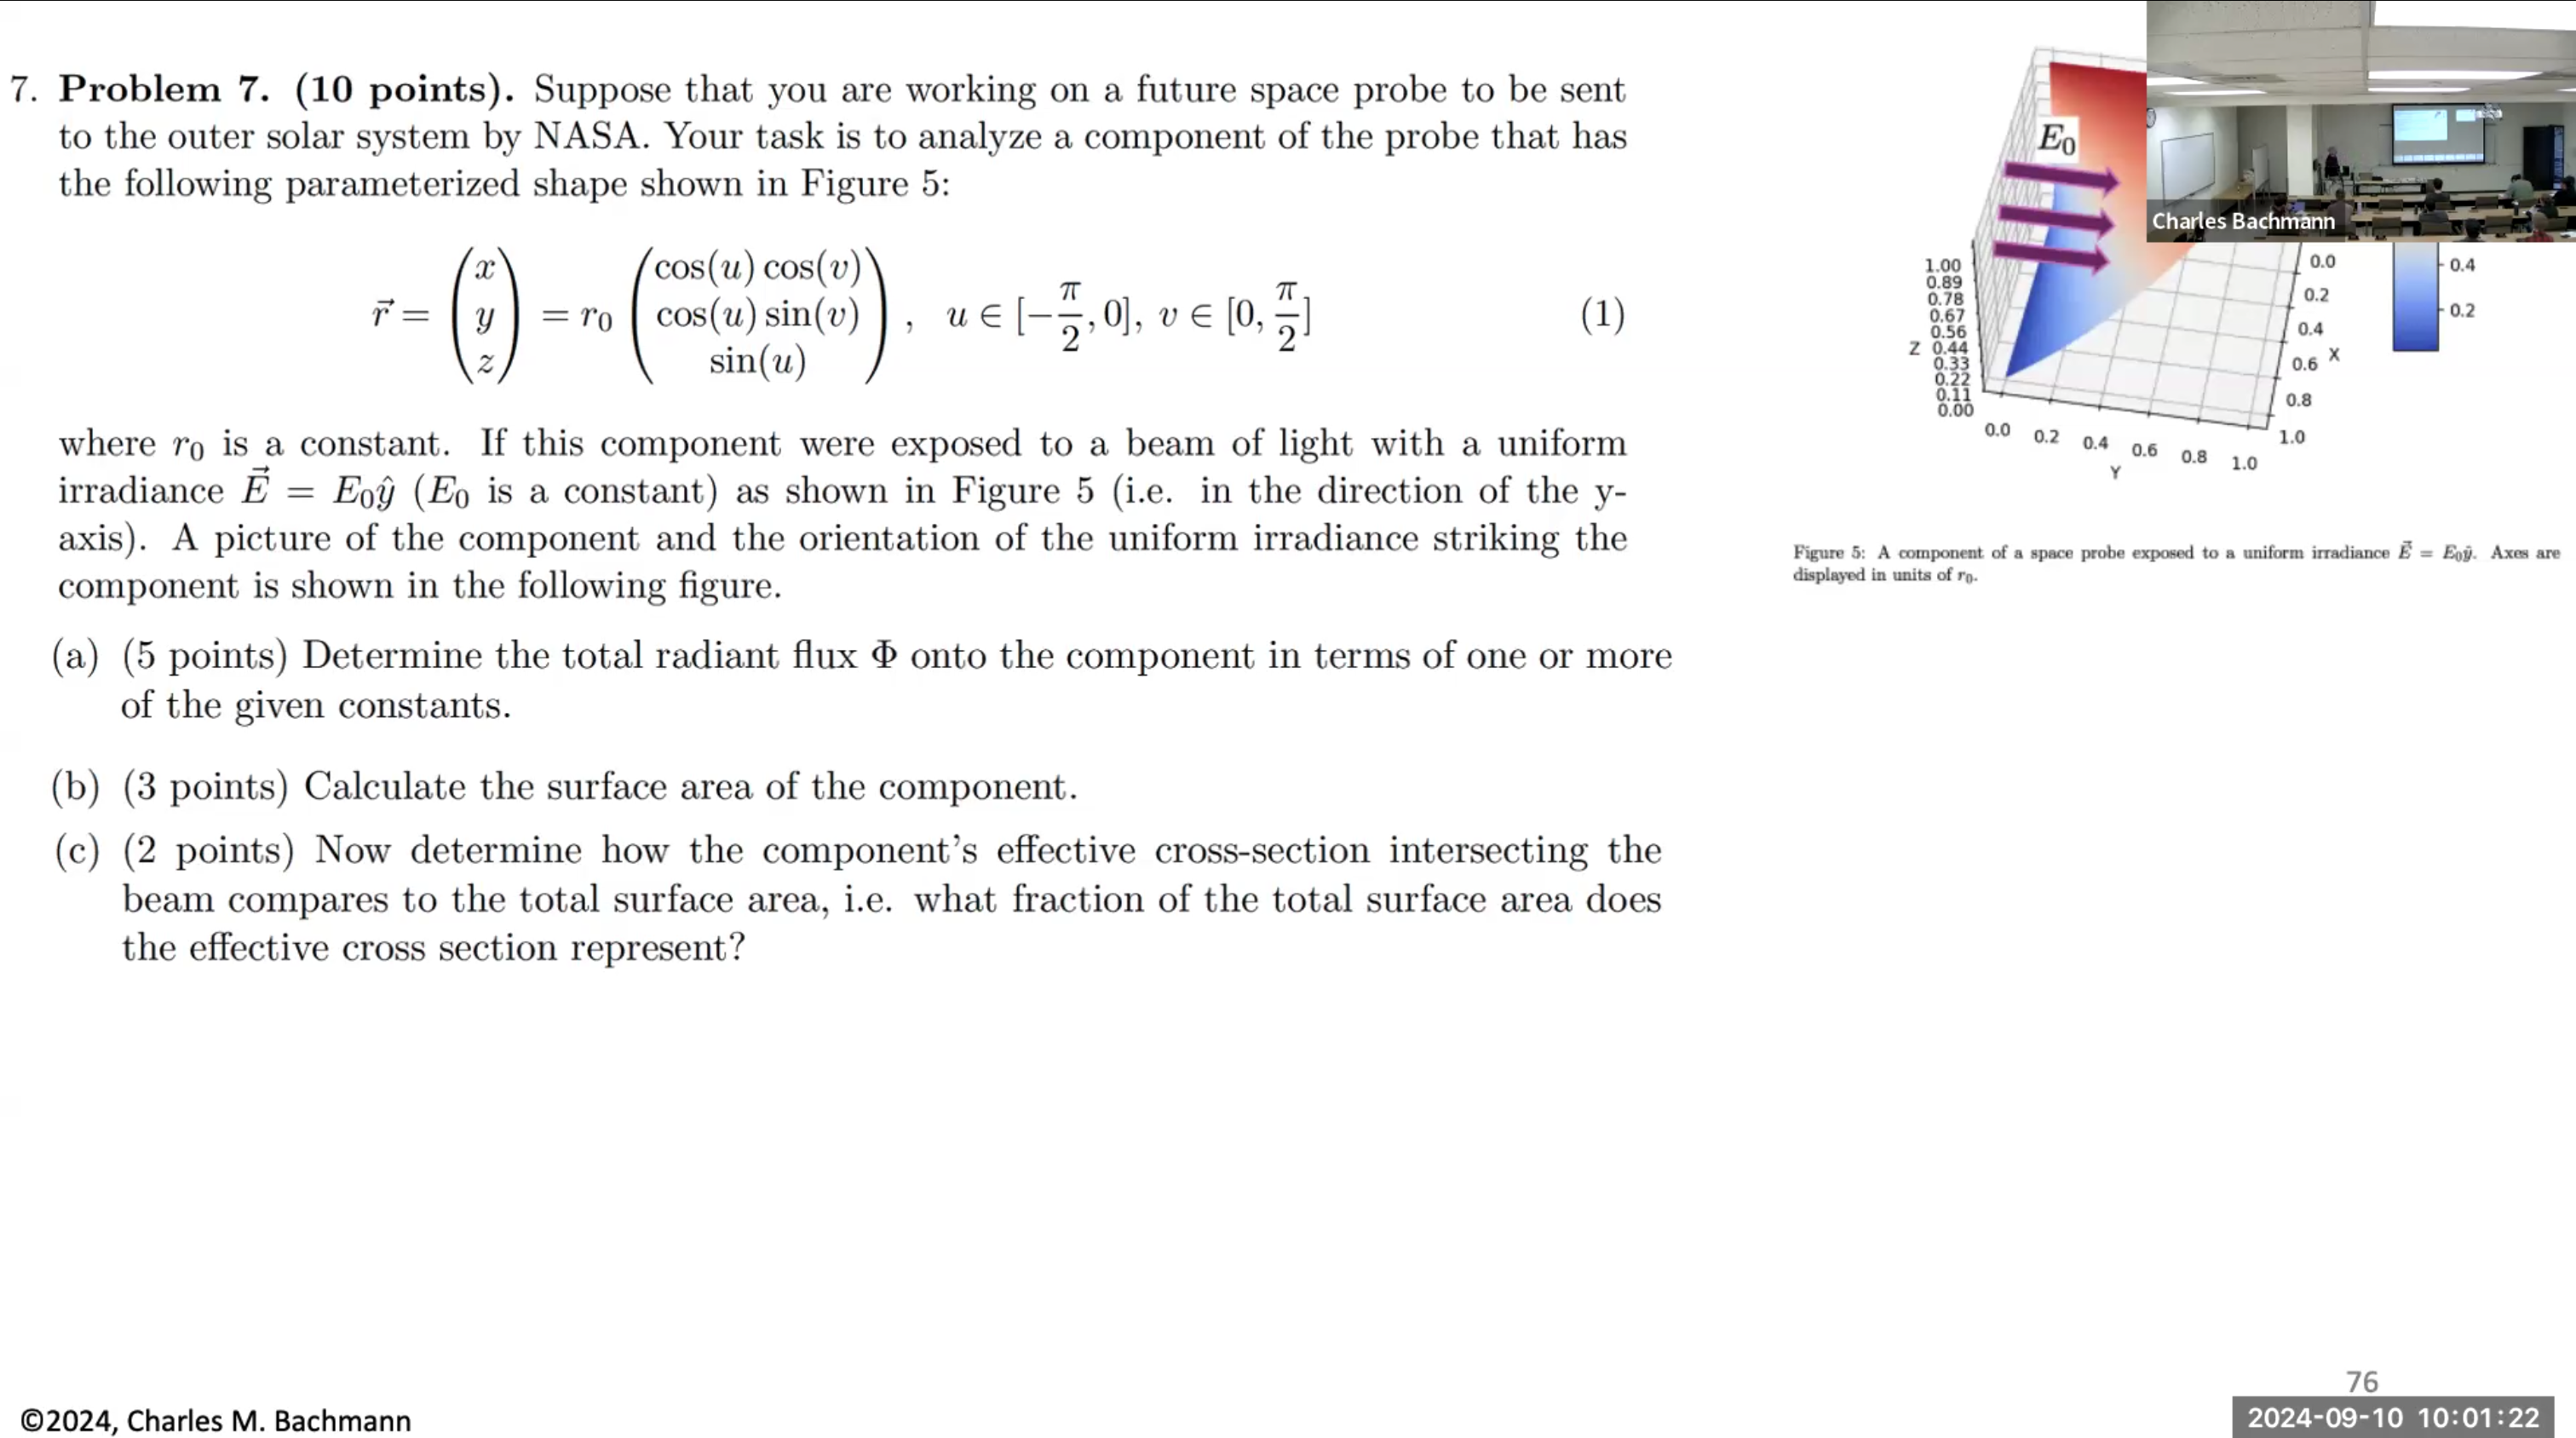
\includegraphics[scale=.4]{Radiometry/Crux/Num1.png}
\caption{NASA Question 7 from Pset 1}
\label{fig:NASA Question}
\end{figure}



\begin{figure}[h!]
\centering
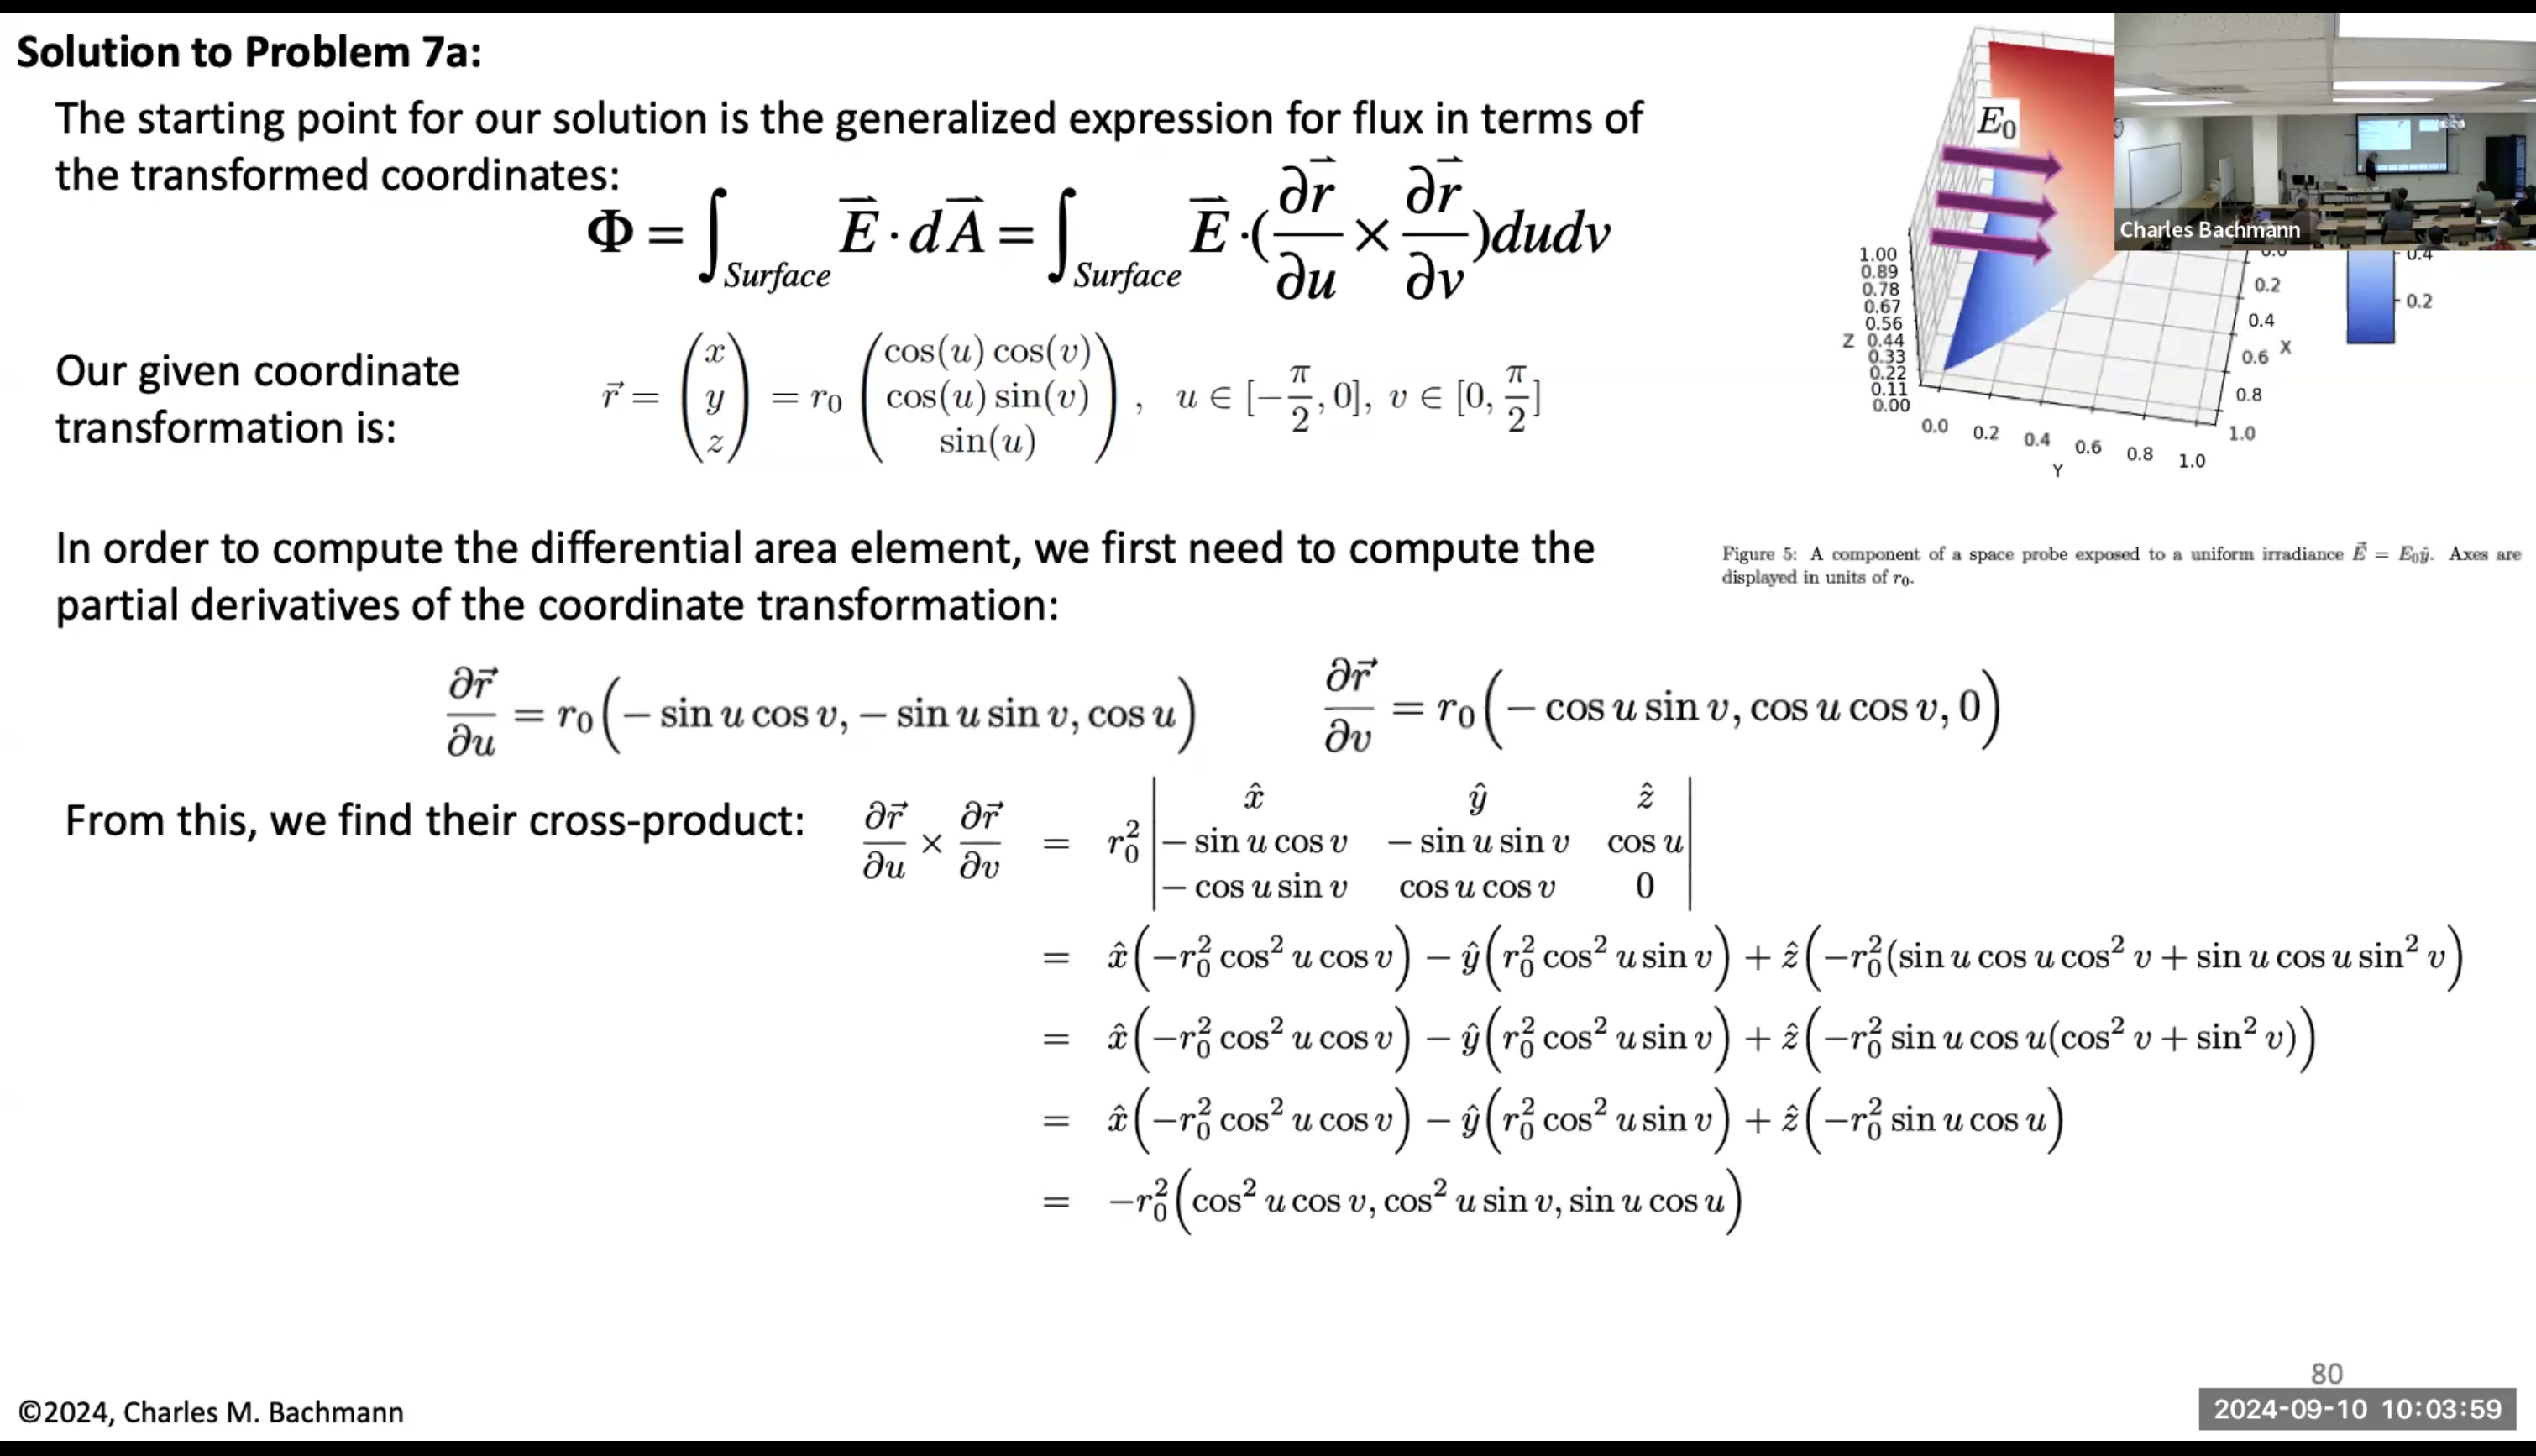
\includegraphics[scale=.4]{Radiometry/Crux/Num2.png}
\caption{NASA Question 7 from Pset 1}
\label{fig:NASA Question}
\end{figure}


\begin{figure}[h!]
\centering
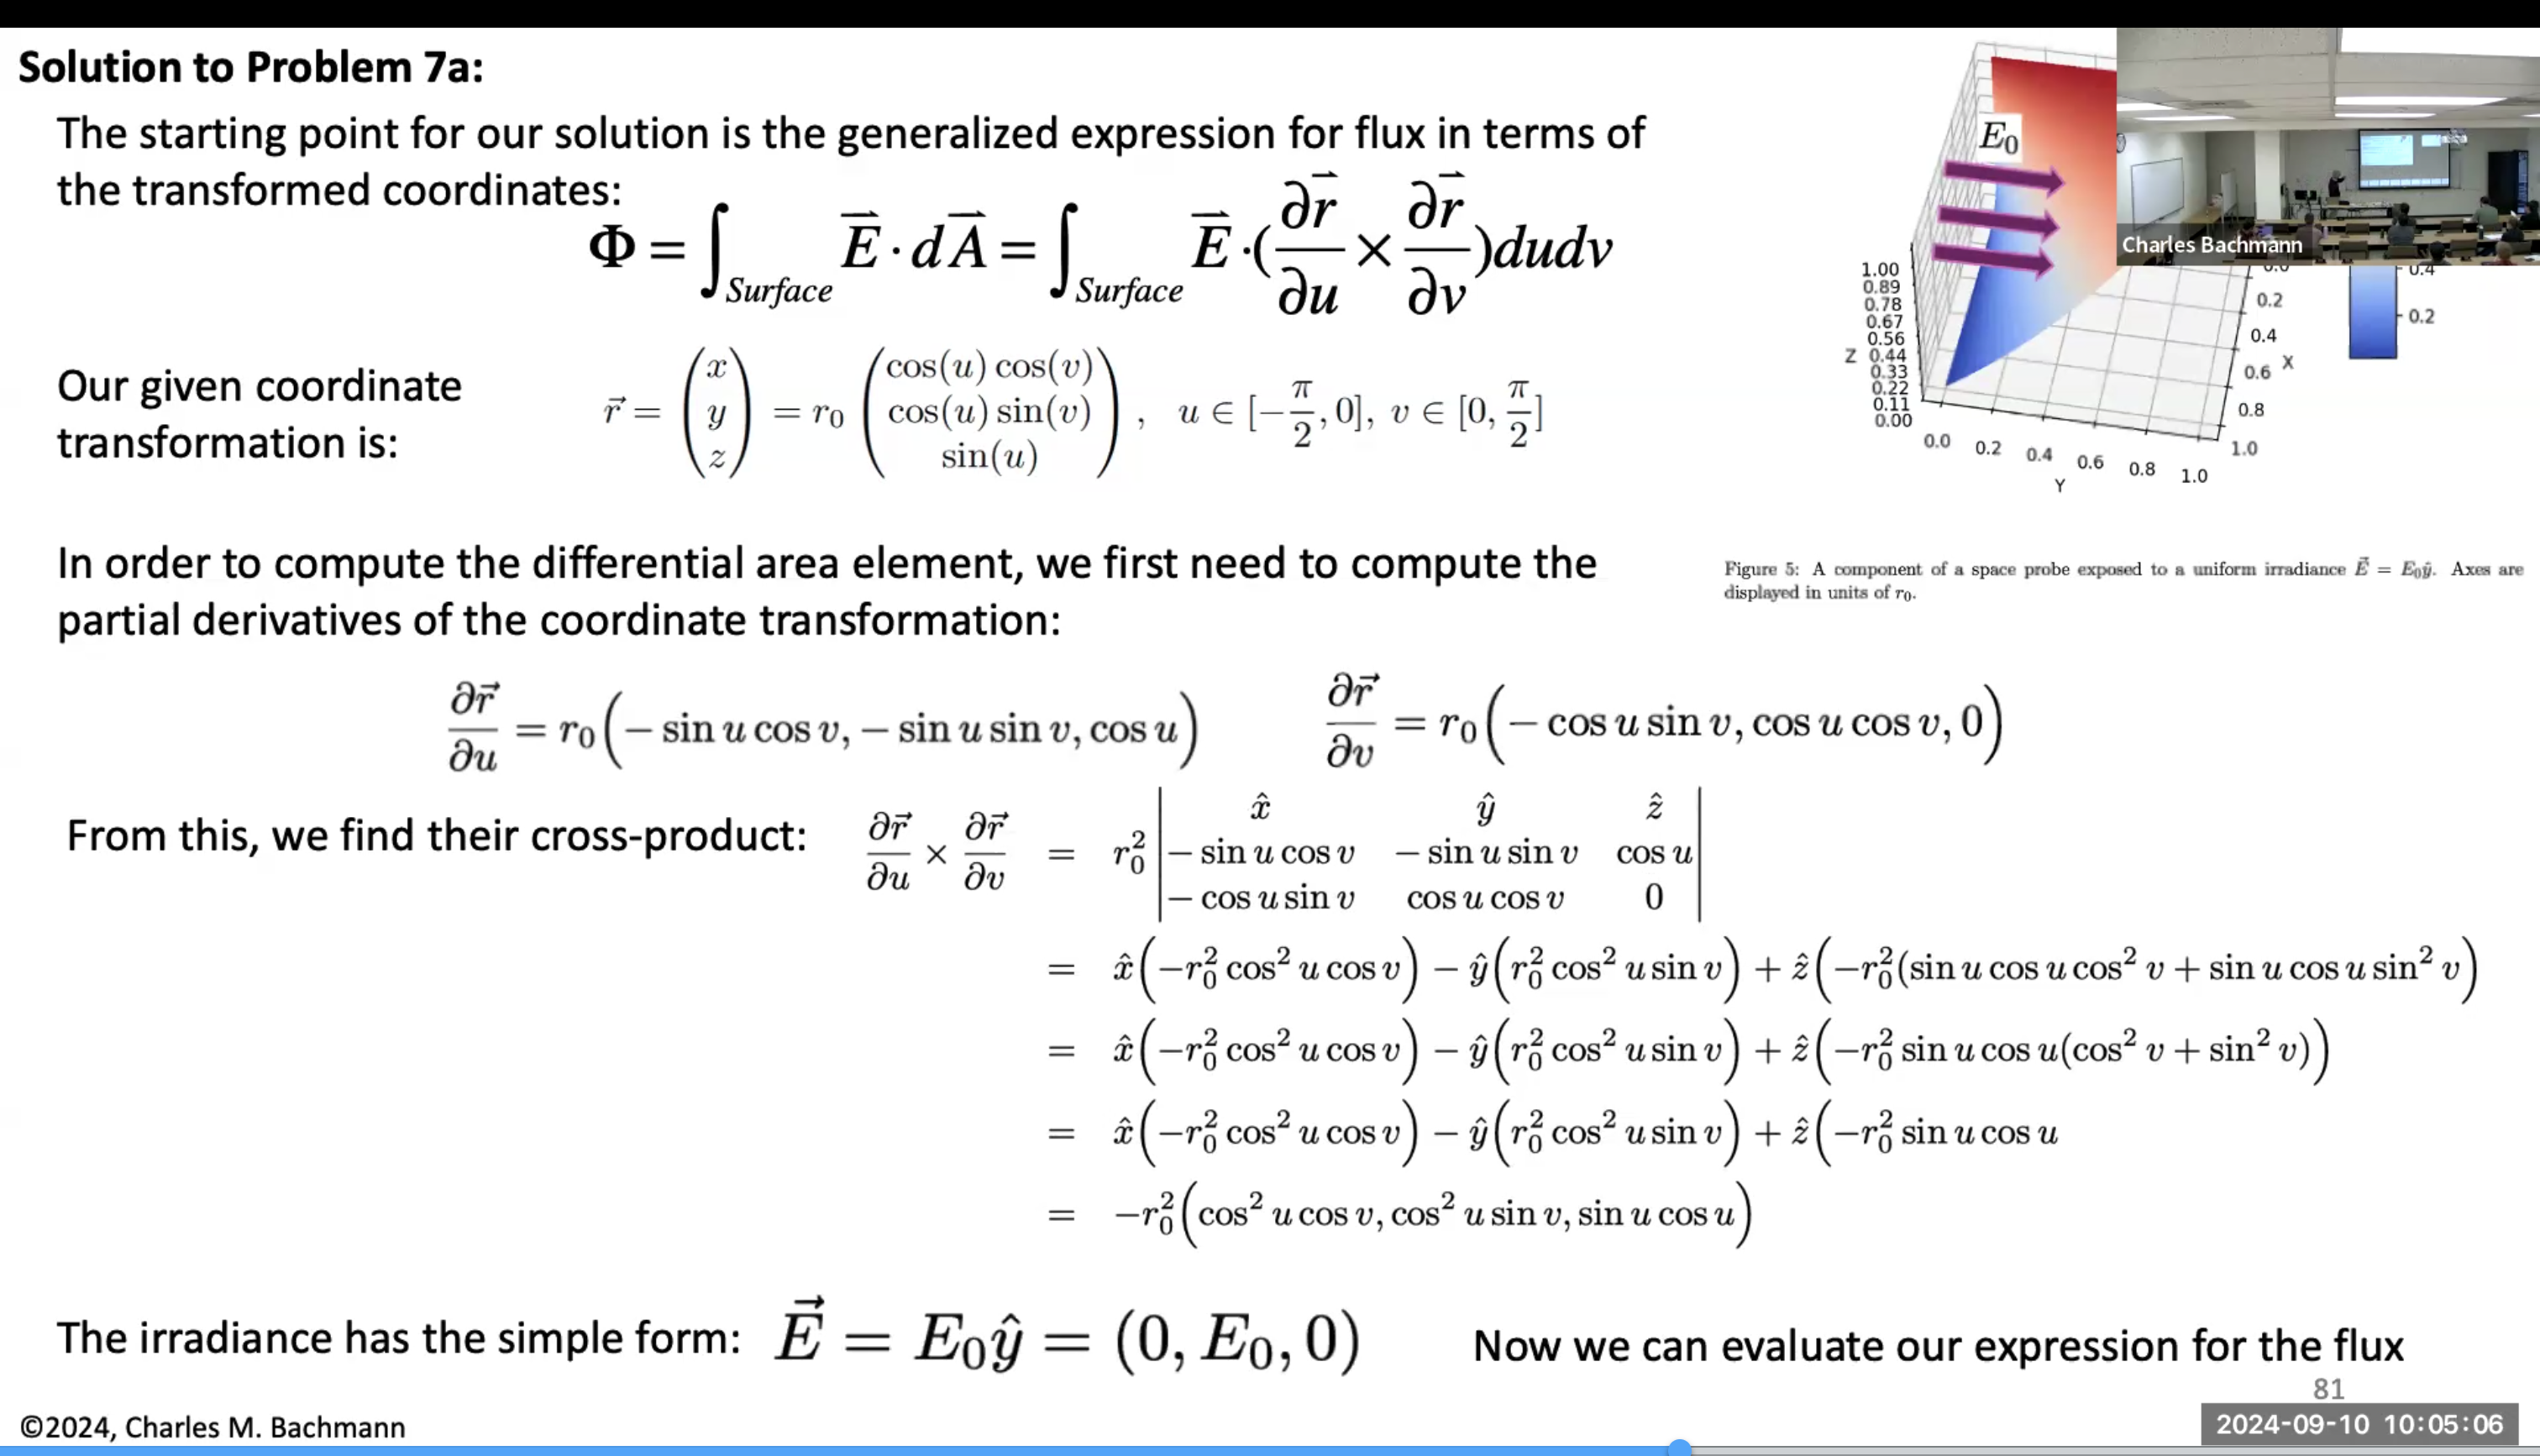
\includegraphics[scale=.4]{Radiometry/Crux/Num3.png}
\caption{NASA Question 7 from Pset 1}
\label{fig:NASA Question}
\end{figure}

\begin{figure}[h!]
\centering
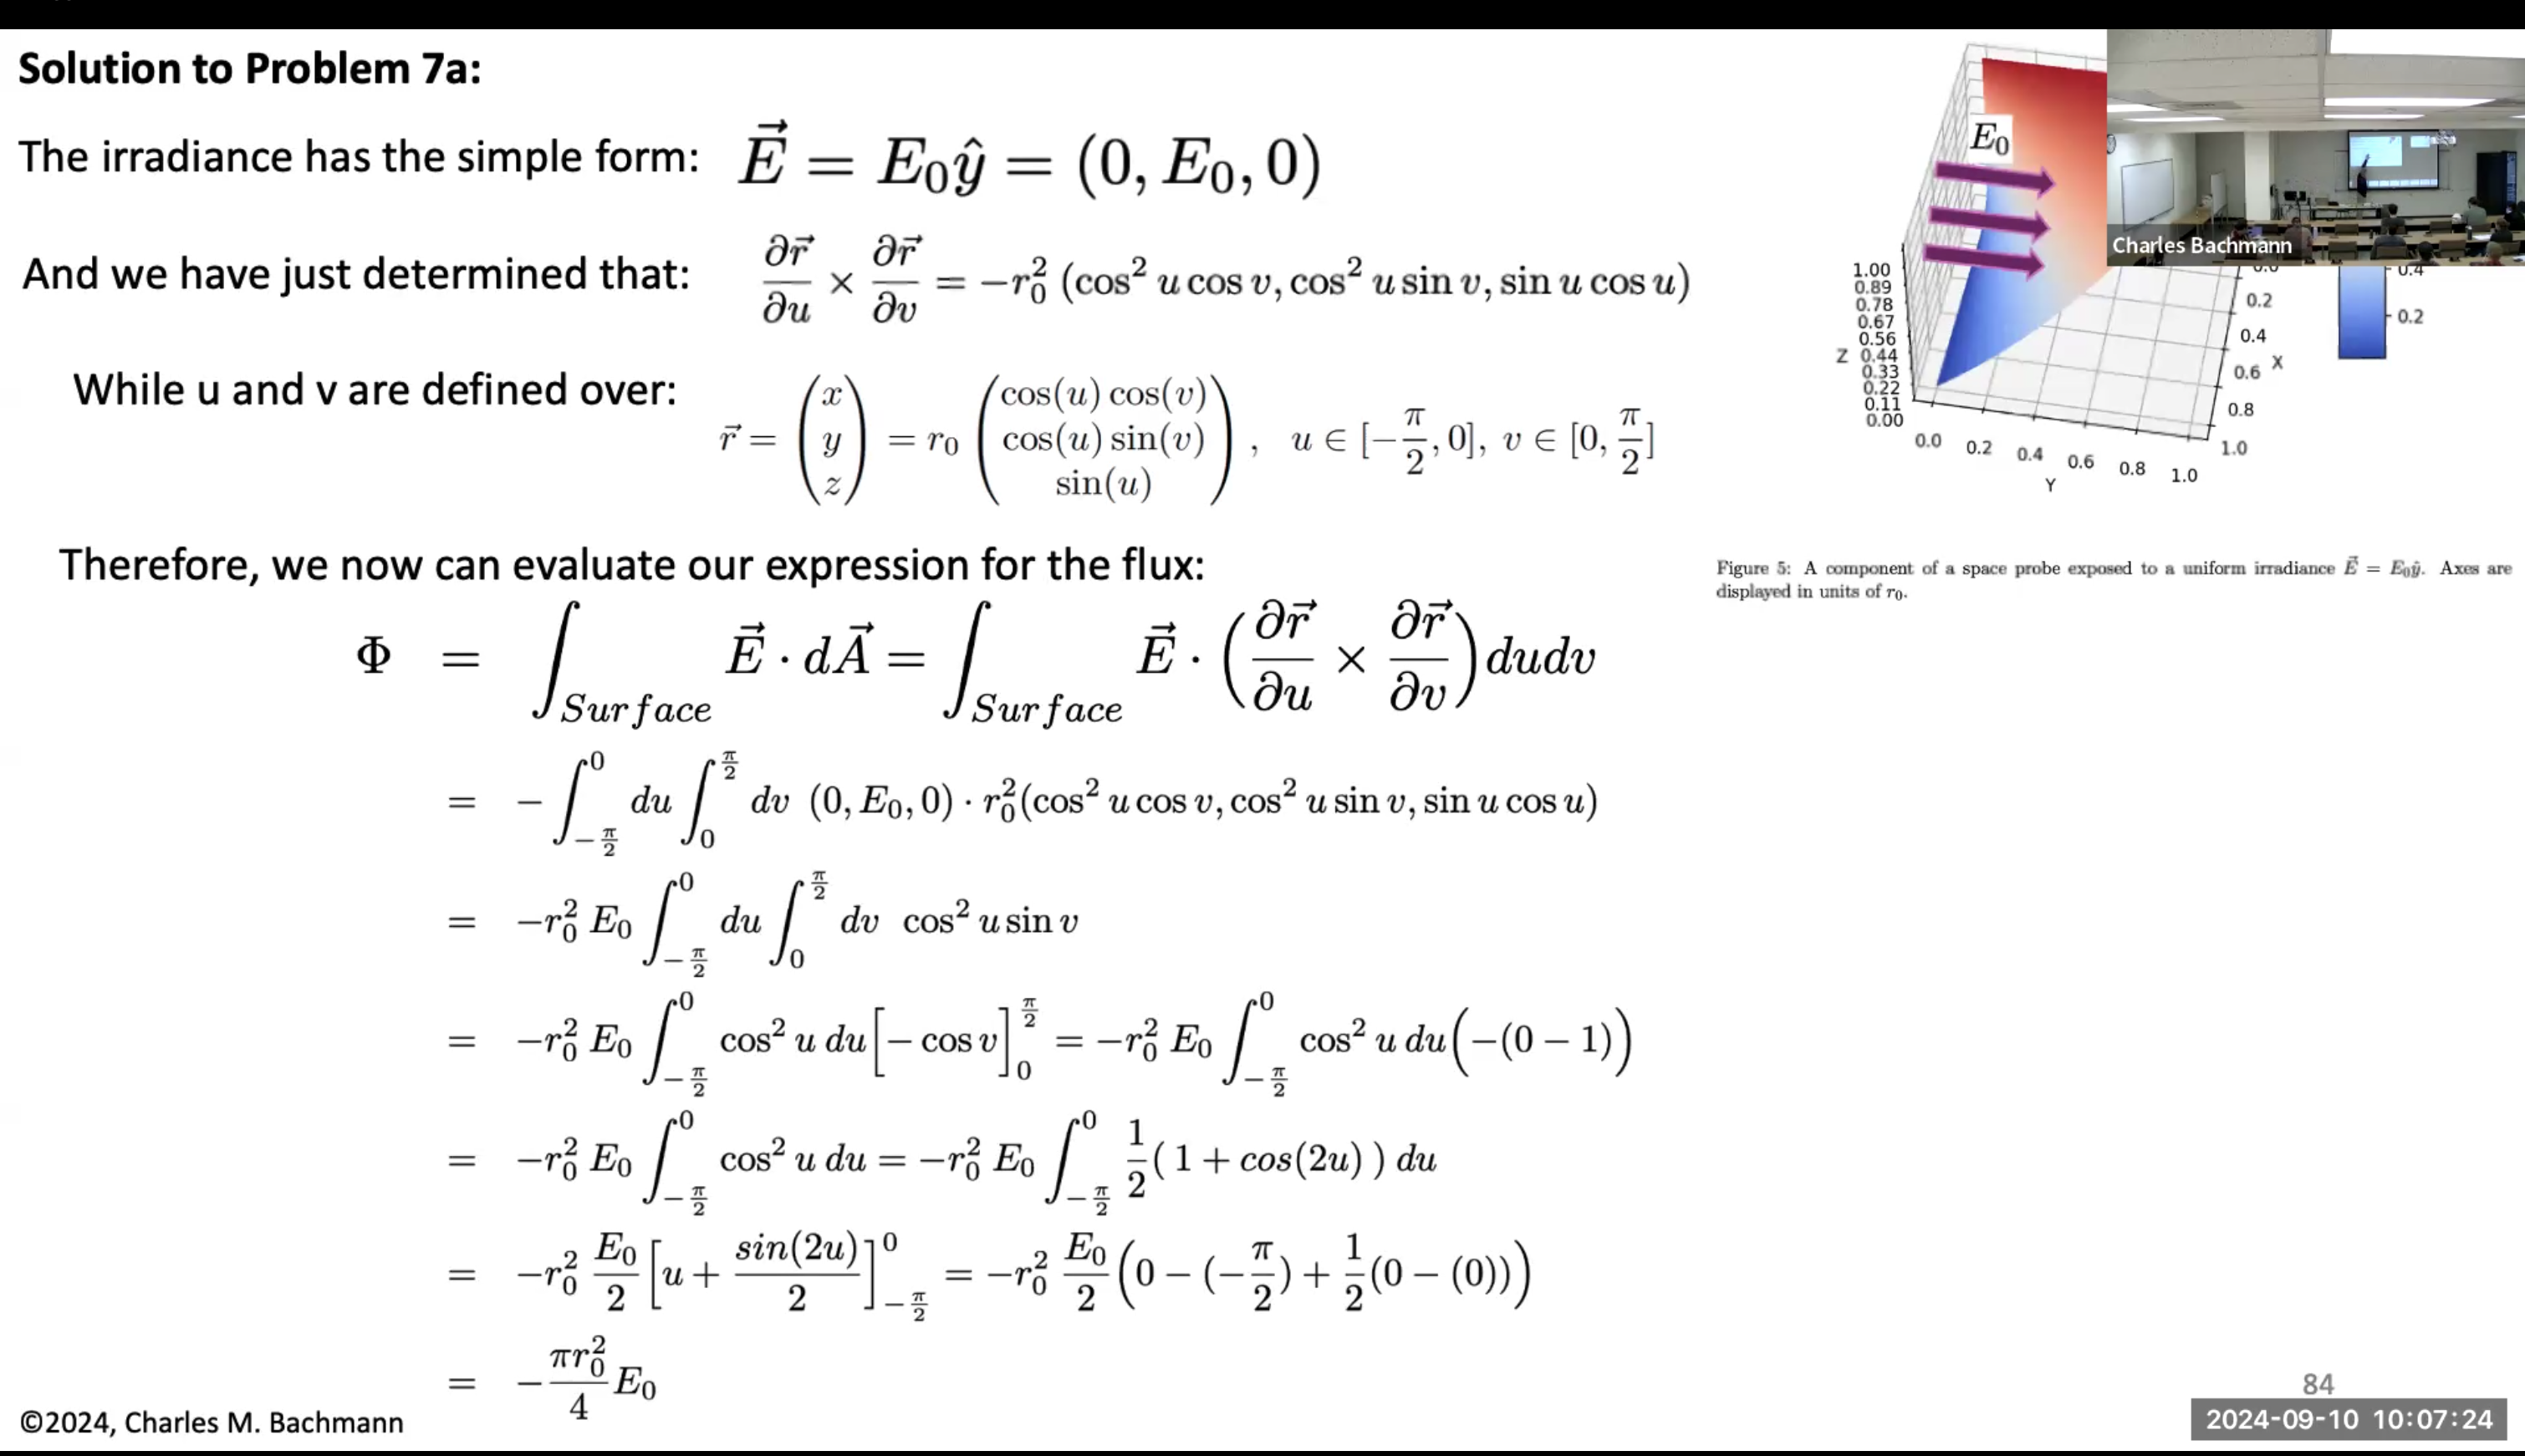
\includegraphics[scale=.4]{Radiometry/Crux/Num4.png}
\caption{NASA Question 7 from Pset 1}
\label{fig:NASA Question}
\end{figure}

\begin{figure}[h!]
\centering
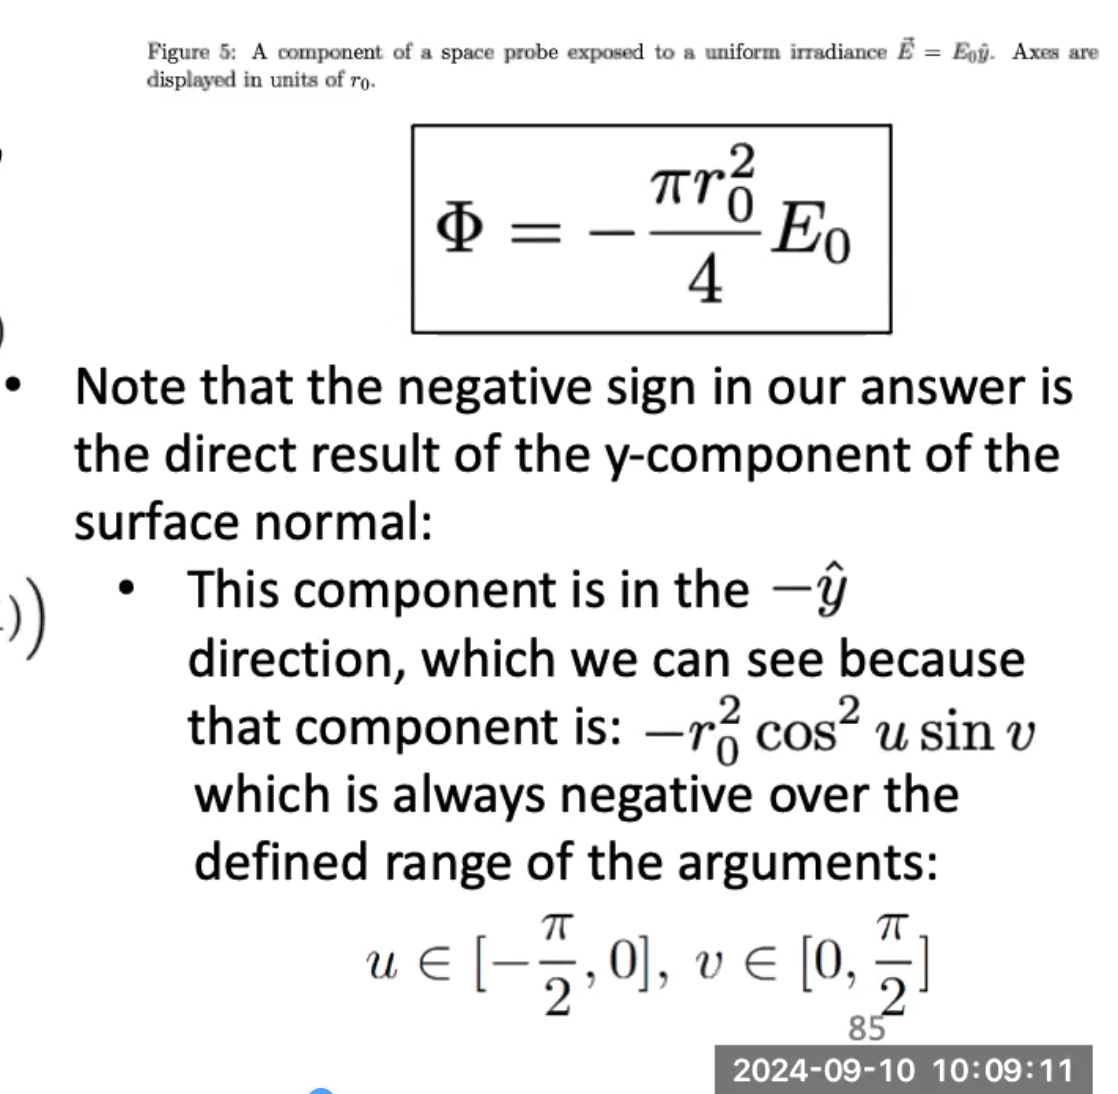
\includegraphics[scale=.3]{Radiometry/Crux/Num5.png}
\caption{NASA Question 7 from Pset 1}
\label{fig:NASA Question}
\end{figure}

\begin{figure}[h!]
\centering
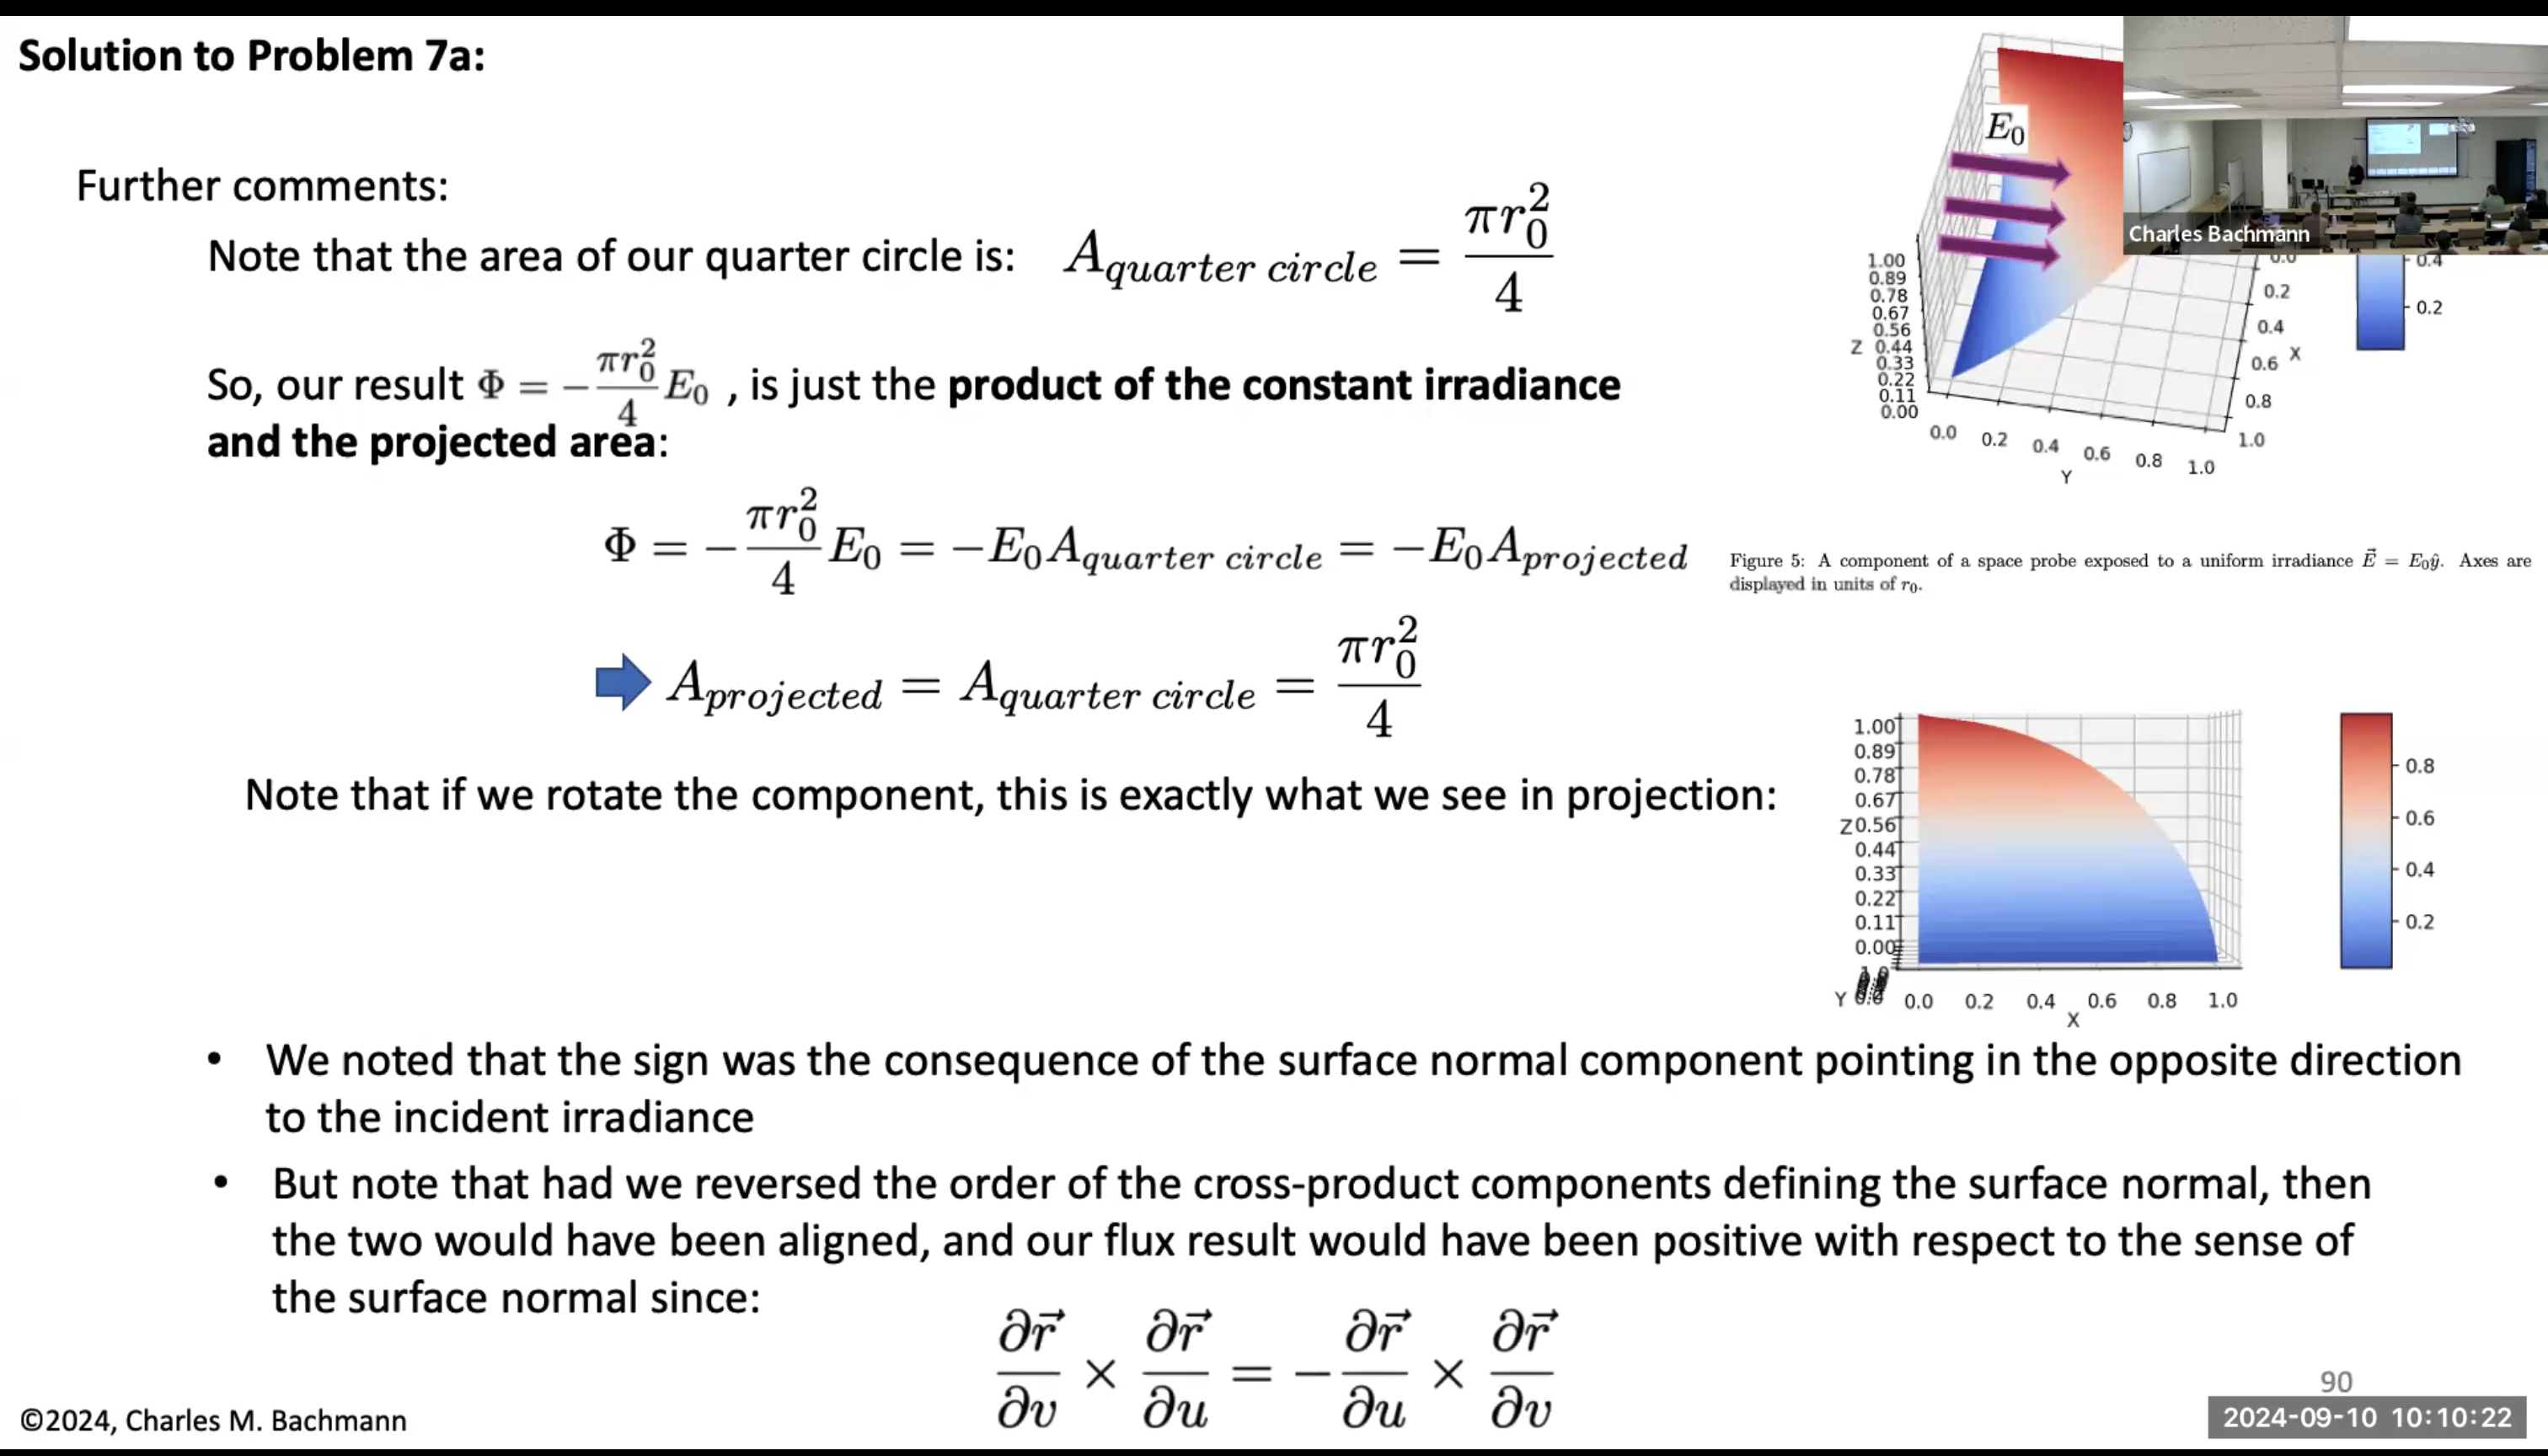
\includegraphics[scale=.4]{Radiometry/Crux/Num6.png}
\caption{NASA Question 7 from Pset 1}
\label{fig:NASA Question}
\end{figure}

\begin{figure}[h!]
\centering
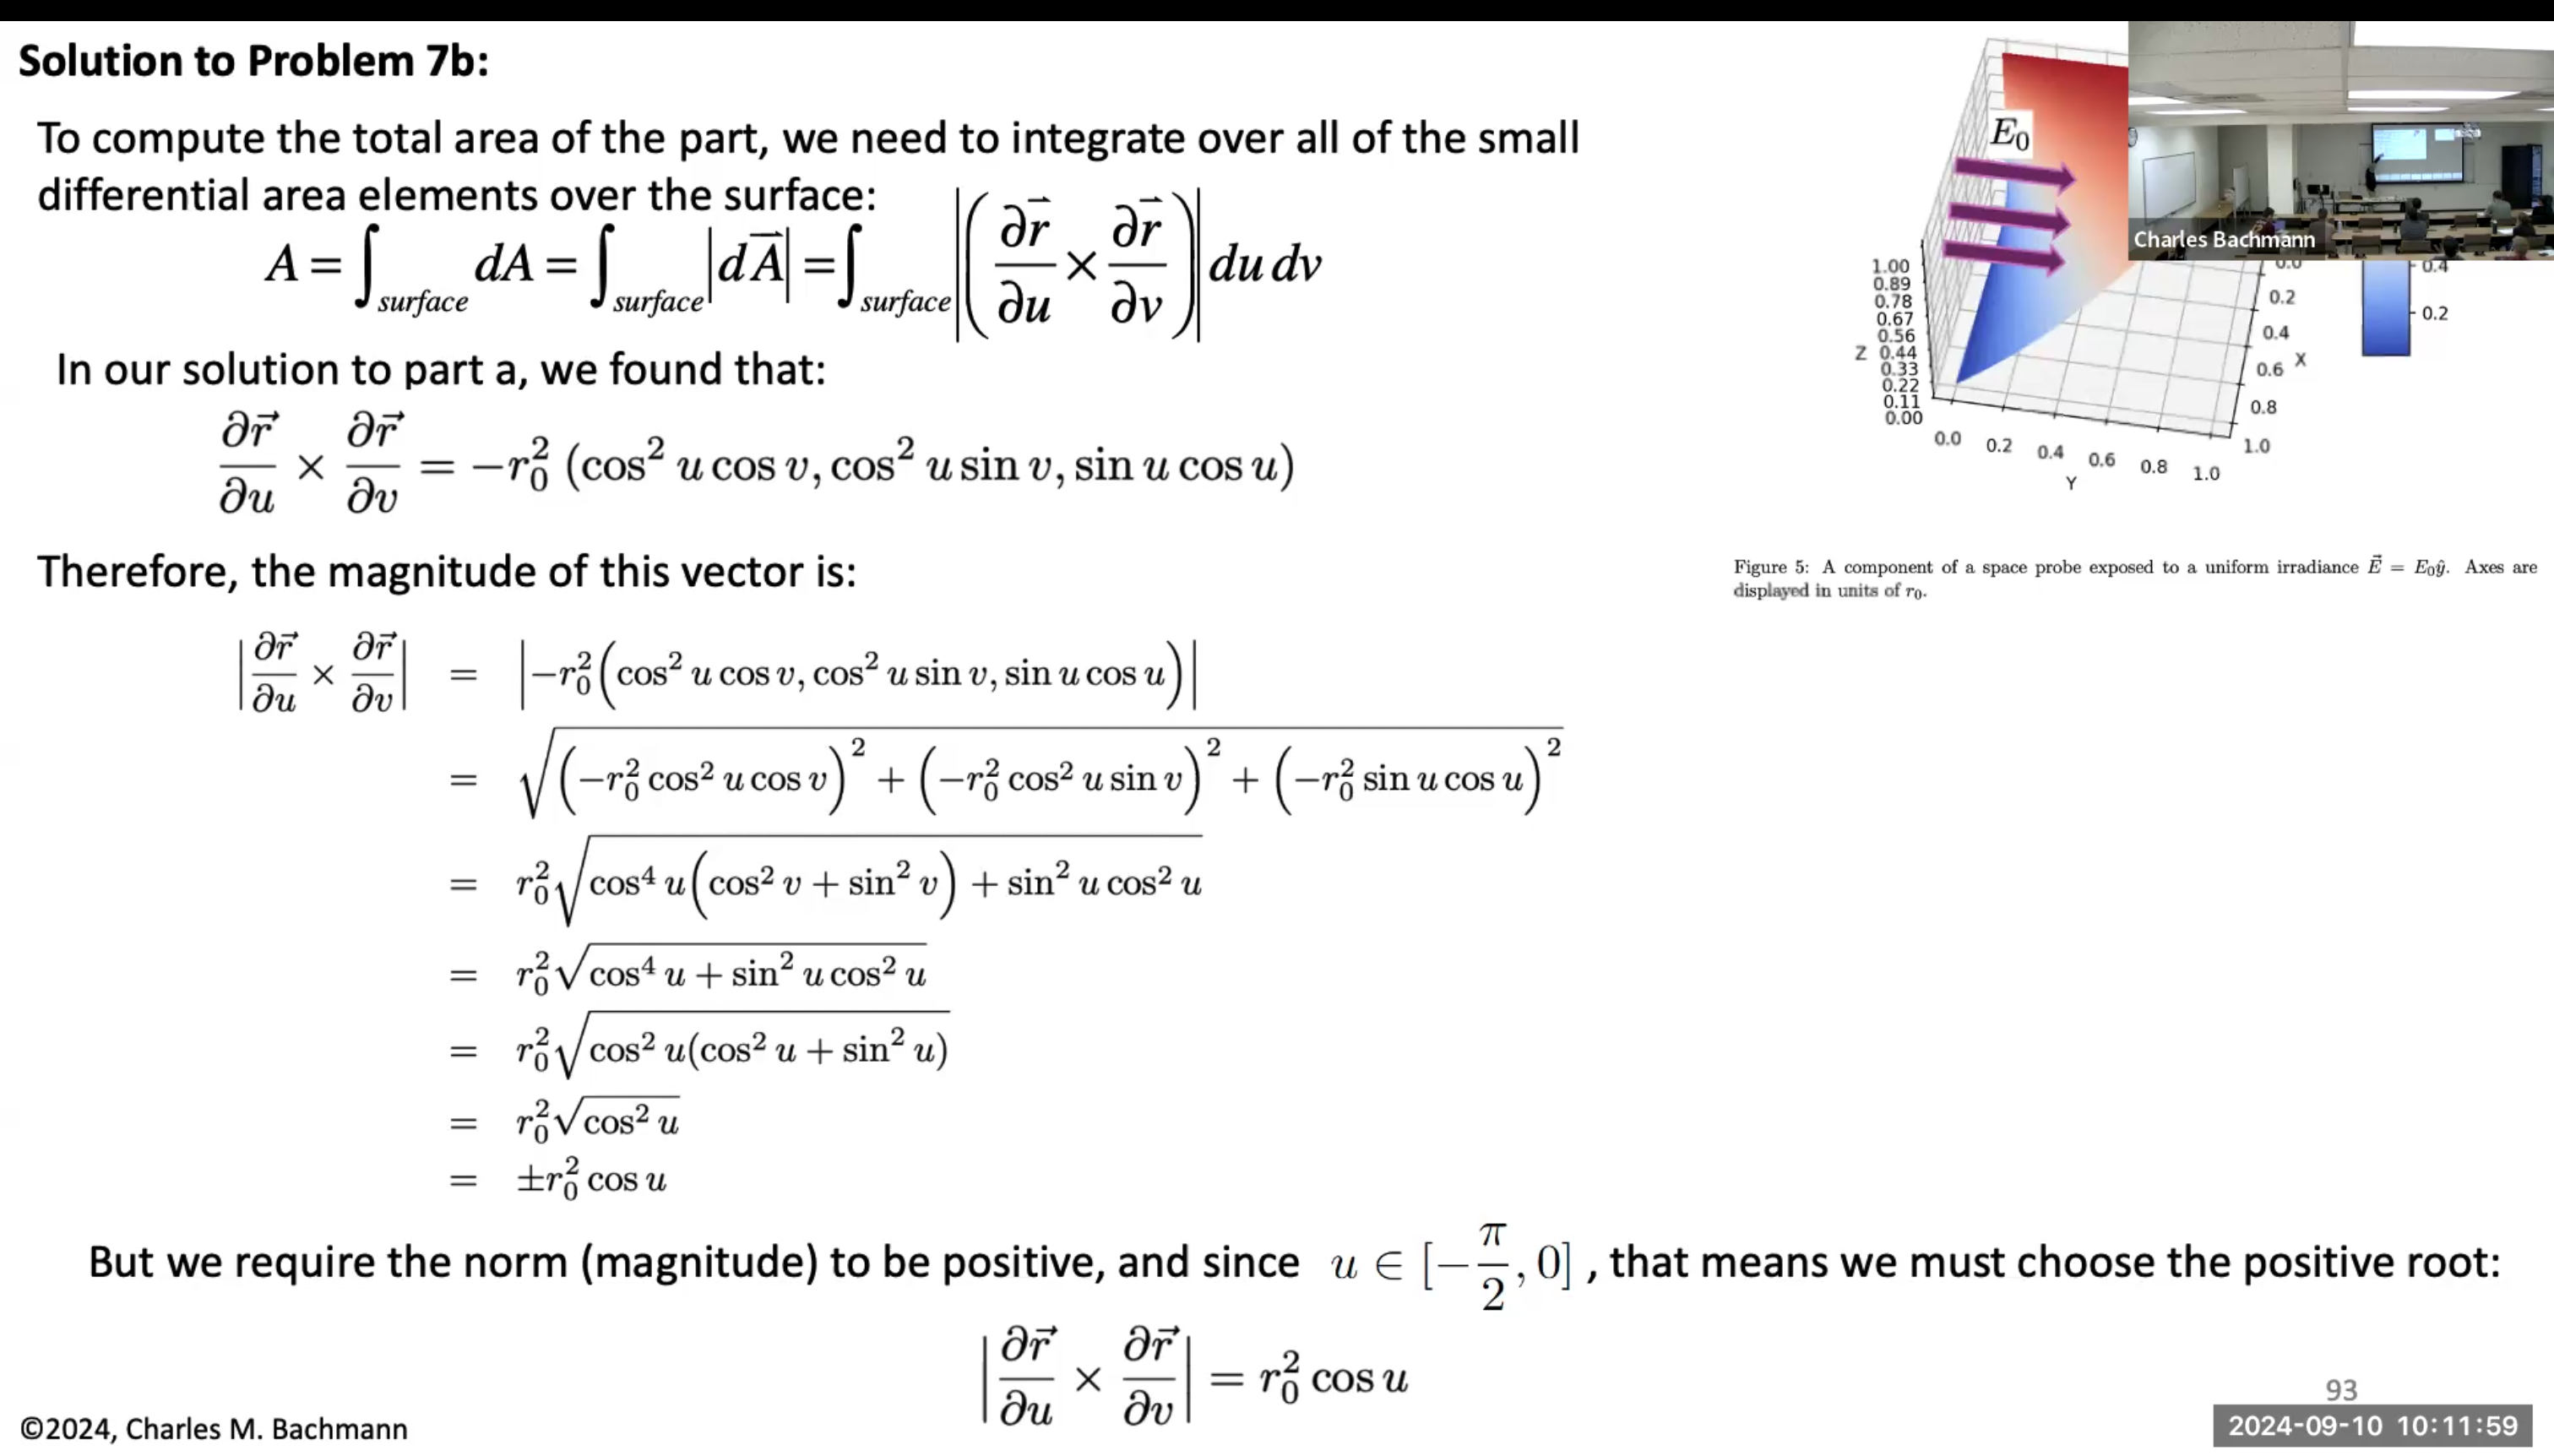
\includegraphics[scale=.4]{Radiometry/Crux/Num7.png}
\caption{NASA Question 7 from Pset 1}
\label{fig:NASA Question}
\end{figure}

\begin{figure}[h!]
\centering
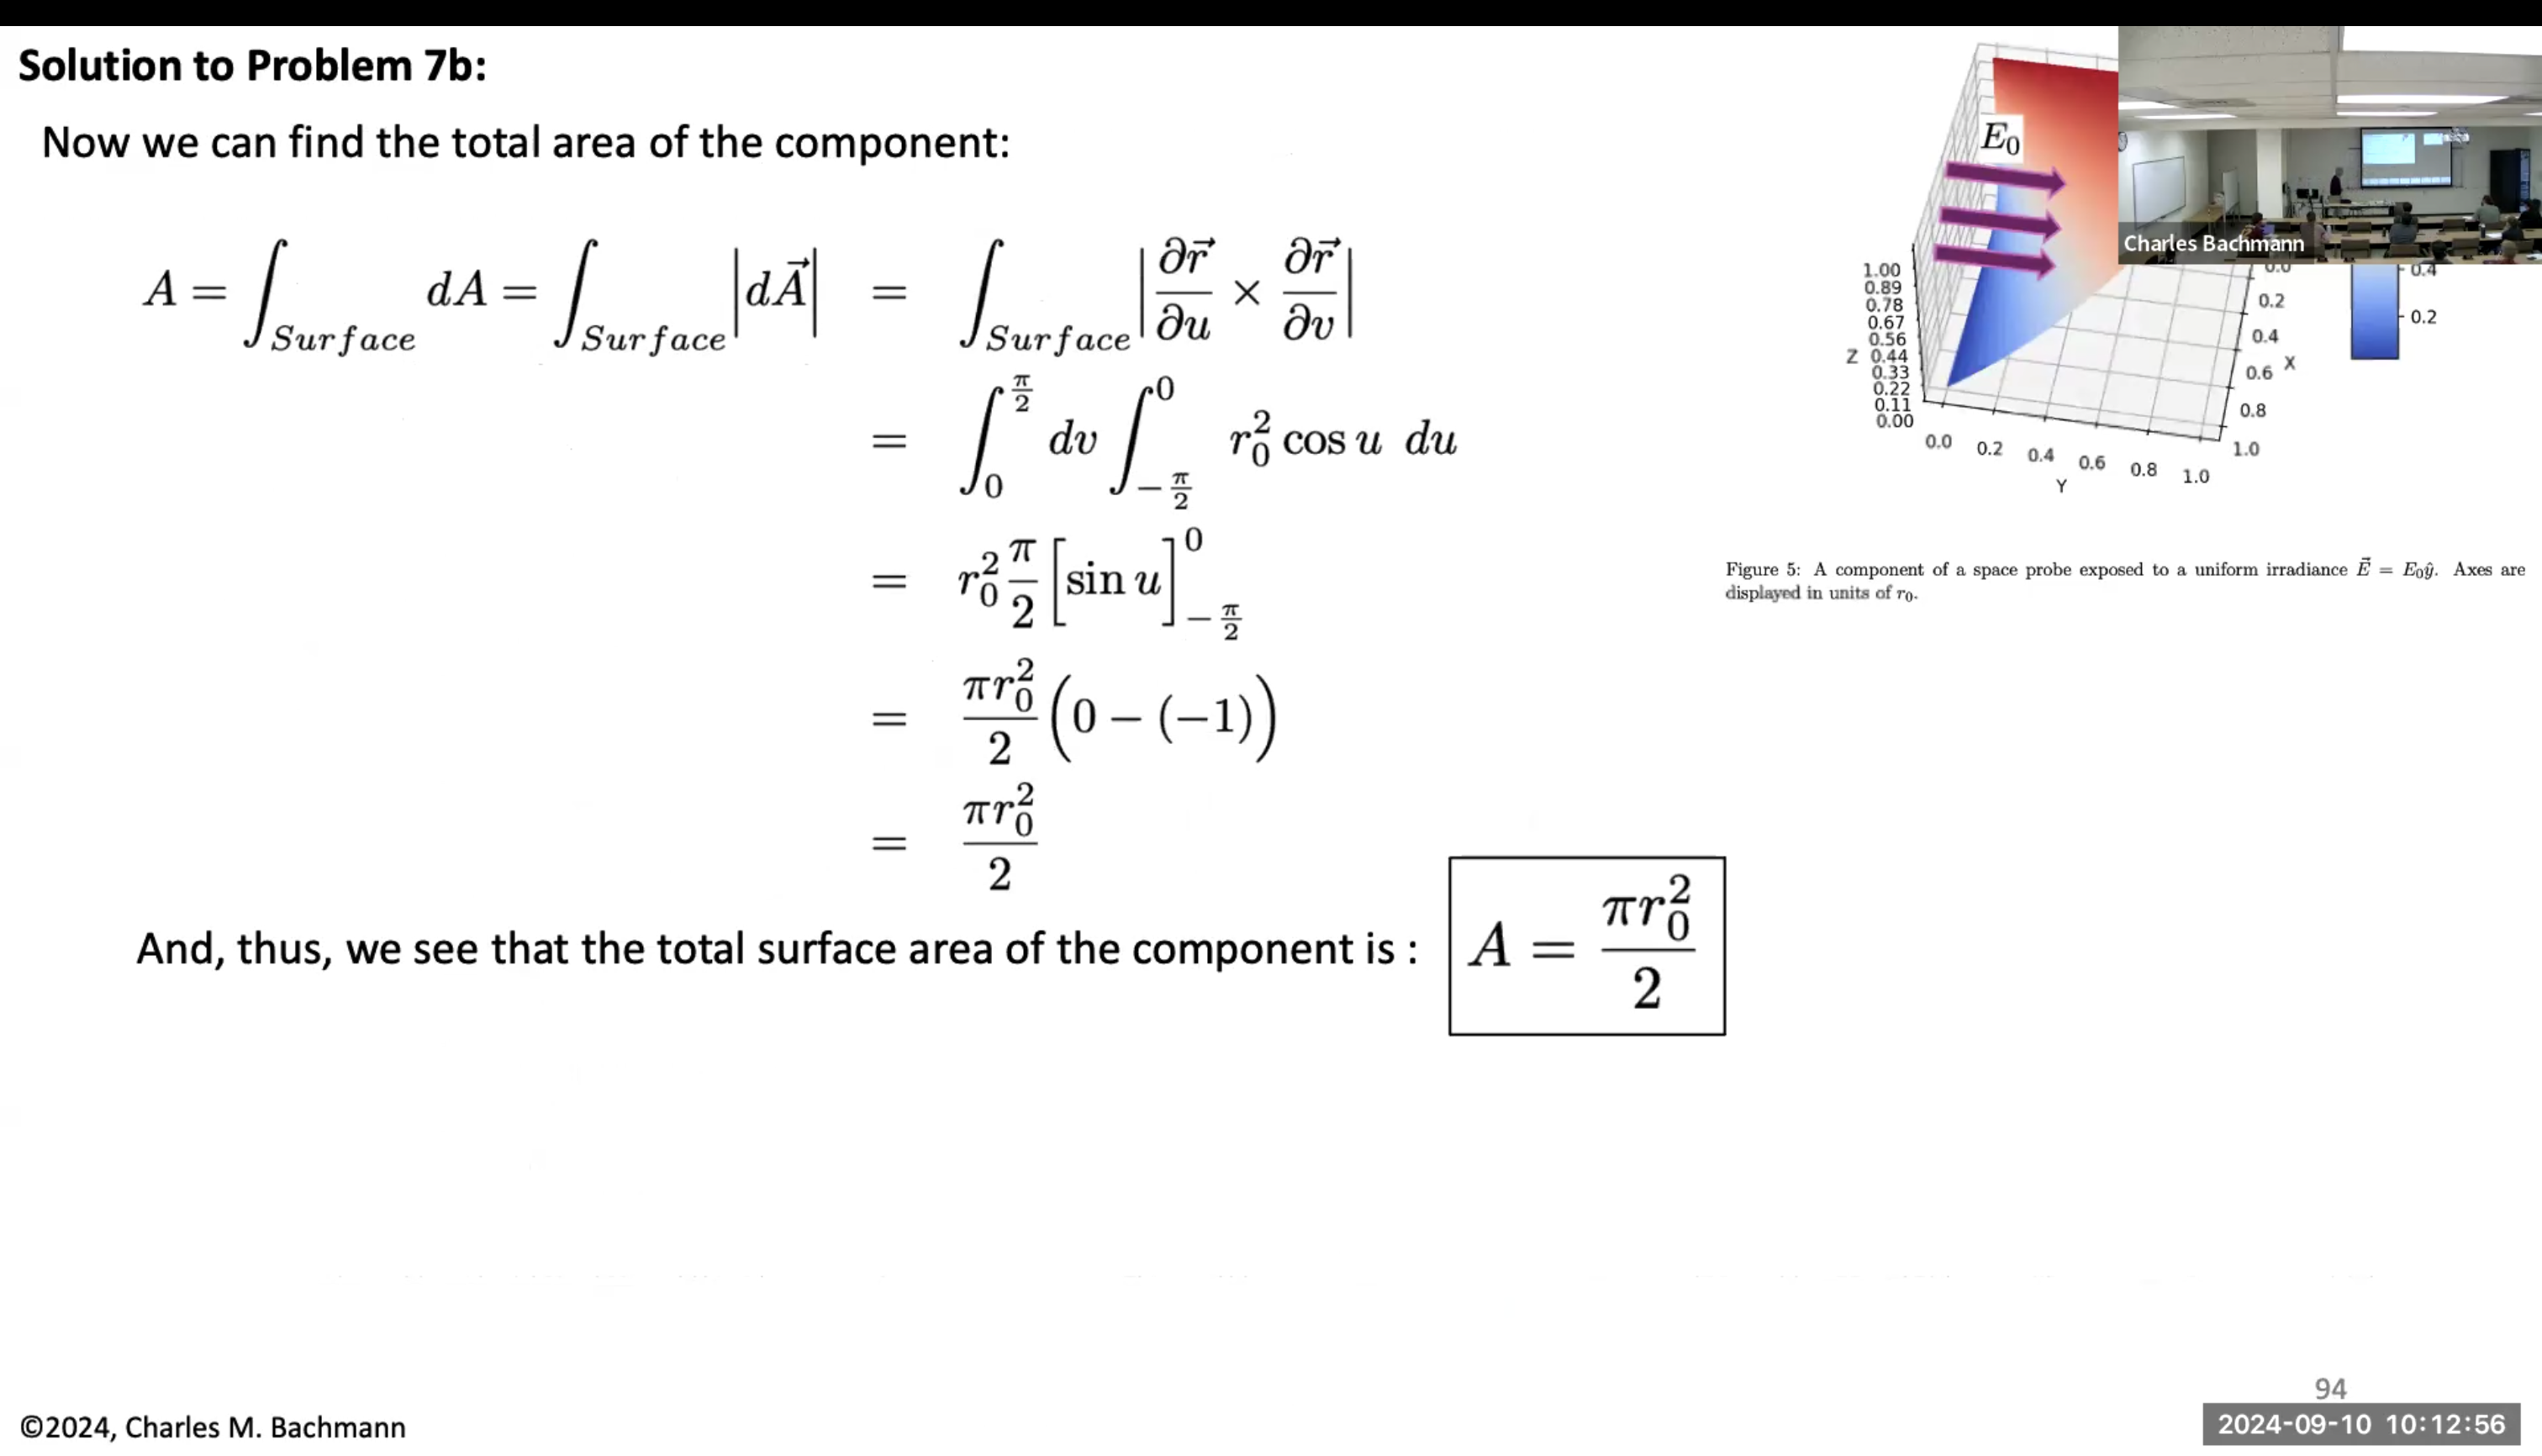
\includegraphics[scale=.4]{Radiometry/Crux/Num8.png}
\caption{NASA Question 7 from Pset 1}
\label{fig:NASA Question}
\end{figure}

\begin{figure}[h!]
\centering
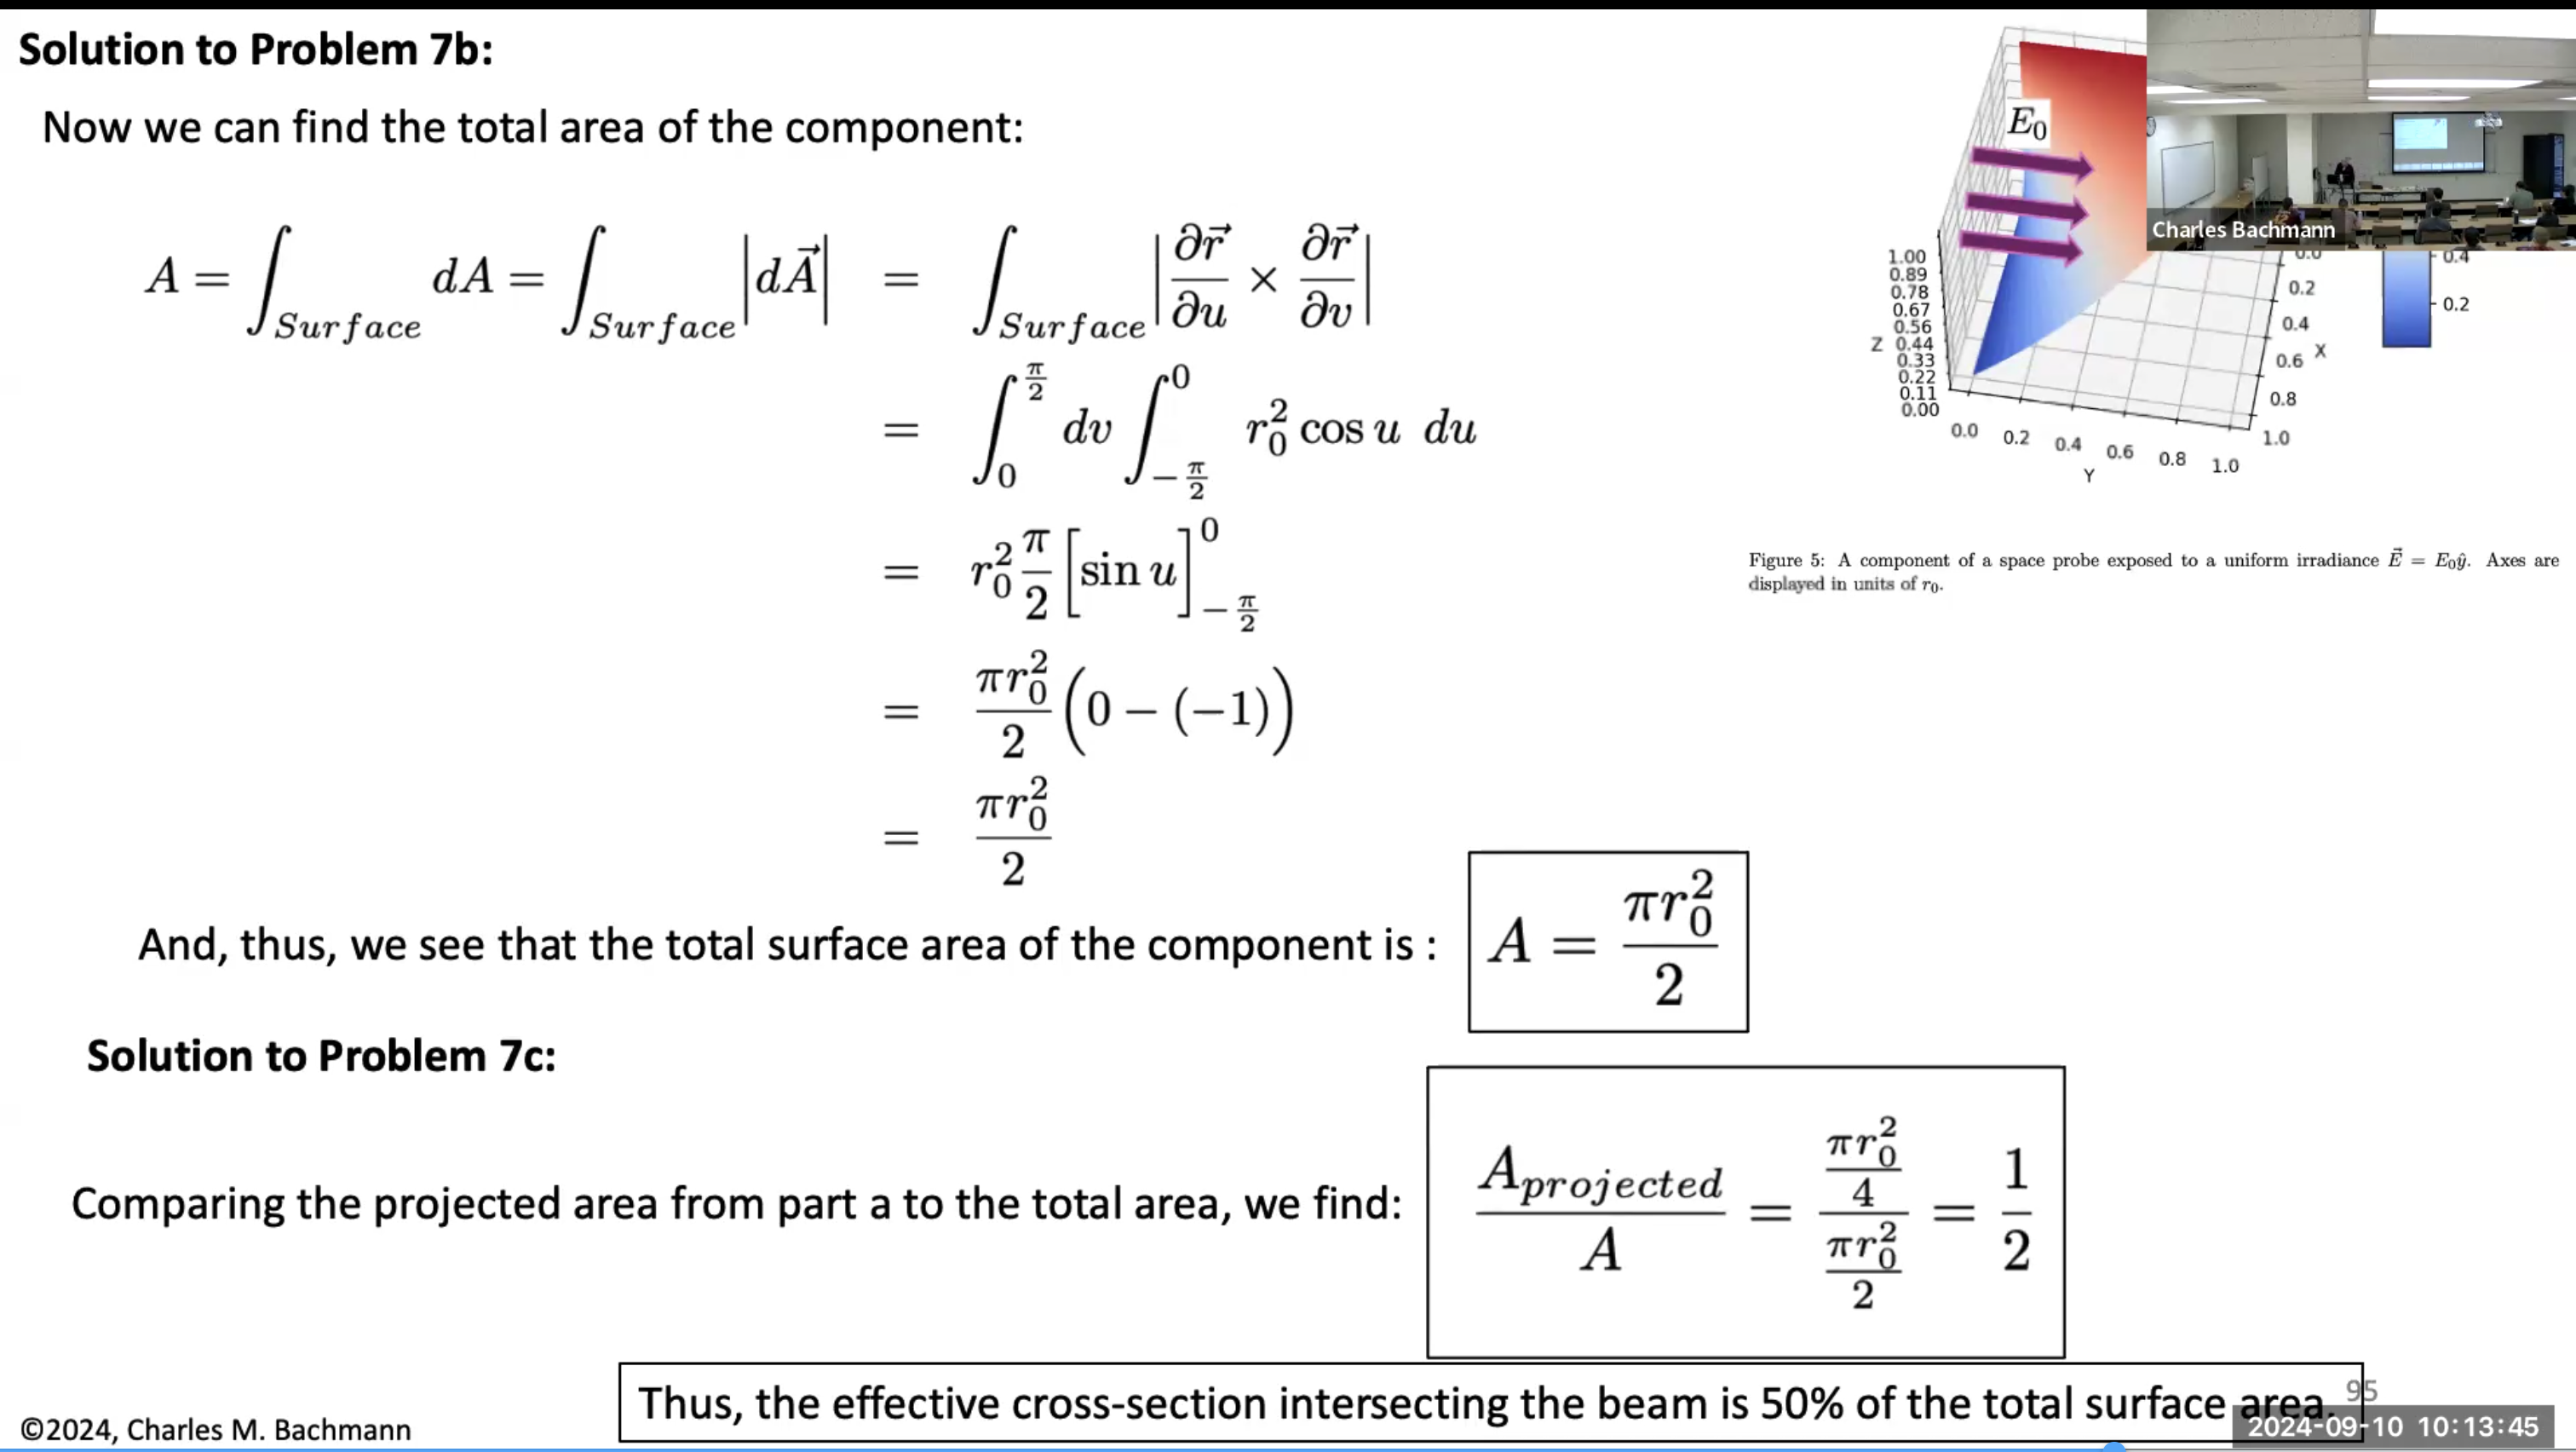
\includegraphics[scale=.4]{Radiometry/Crux/Num9.png}
\caption{NASA Question 7 from Pset 1}
\label{fig:NASA Question}
\end{figure}

\clearpage


\section{Wednesday Review}


\subsection{September 12th, 2024}

Extended source and flux calculations

ds = (opp)(d phi)= r tan theta d phi 
a= (d)(d theta)

Flux = E perpendicular A of radius = A radius L int 0 to 2 pi 0 to theta 1/2 cos theta sin theta d theta d phi 

sin theta 1/2 = R/sqrt (R^2 +r^2)

\begin{figure}[h!]
\centering
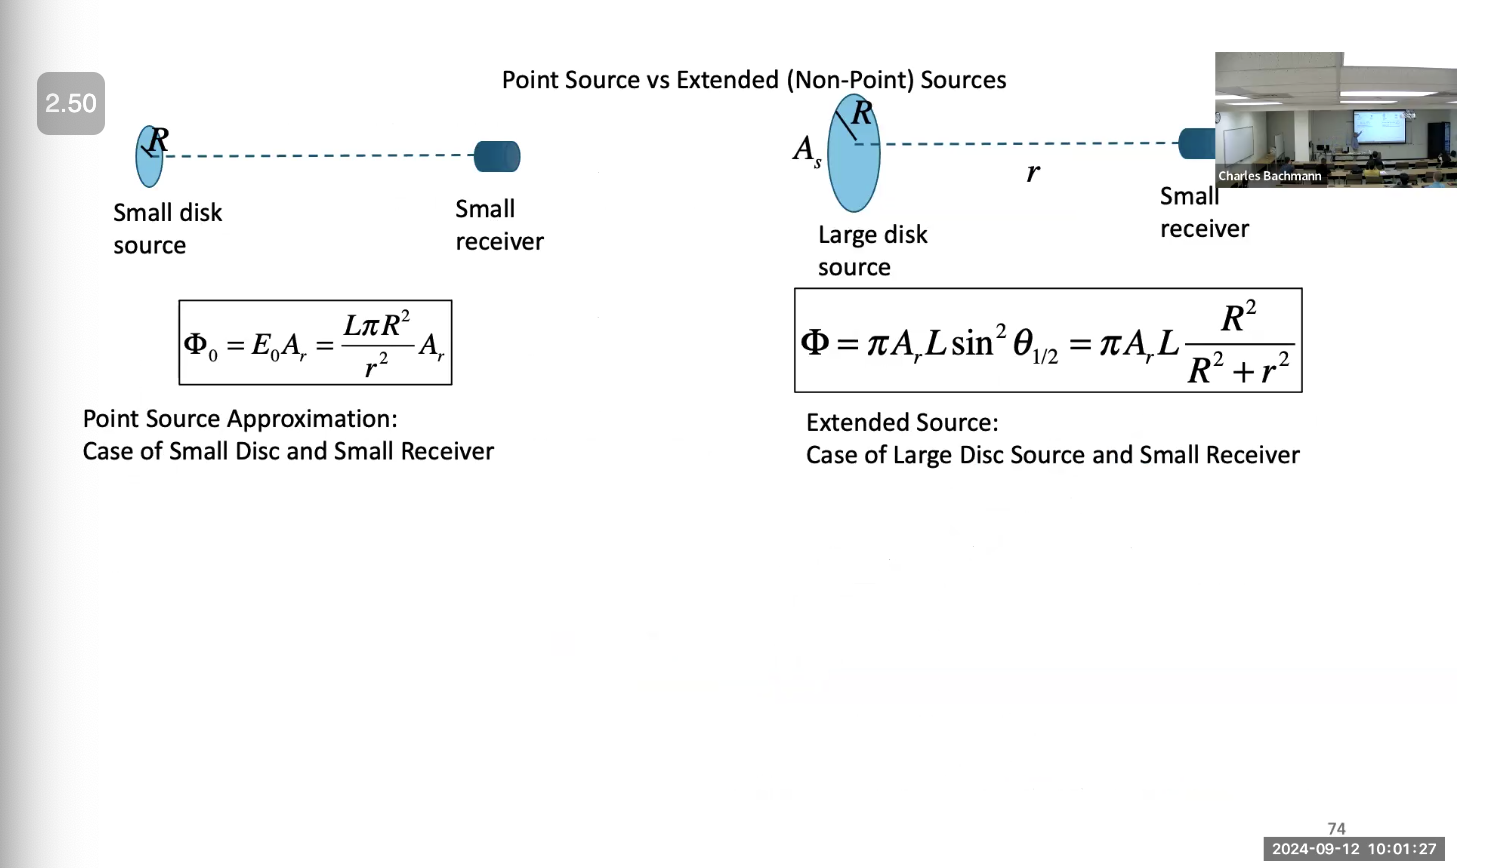
\includegraphics[scale=.6]{Radiometry/Week3/Notes/sept12th.png}
\caption{Nugget the Snowman}
\label{fig:Sept 12}
\end{figure}

\begin{figure}[h!]
\centering
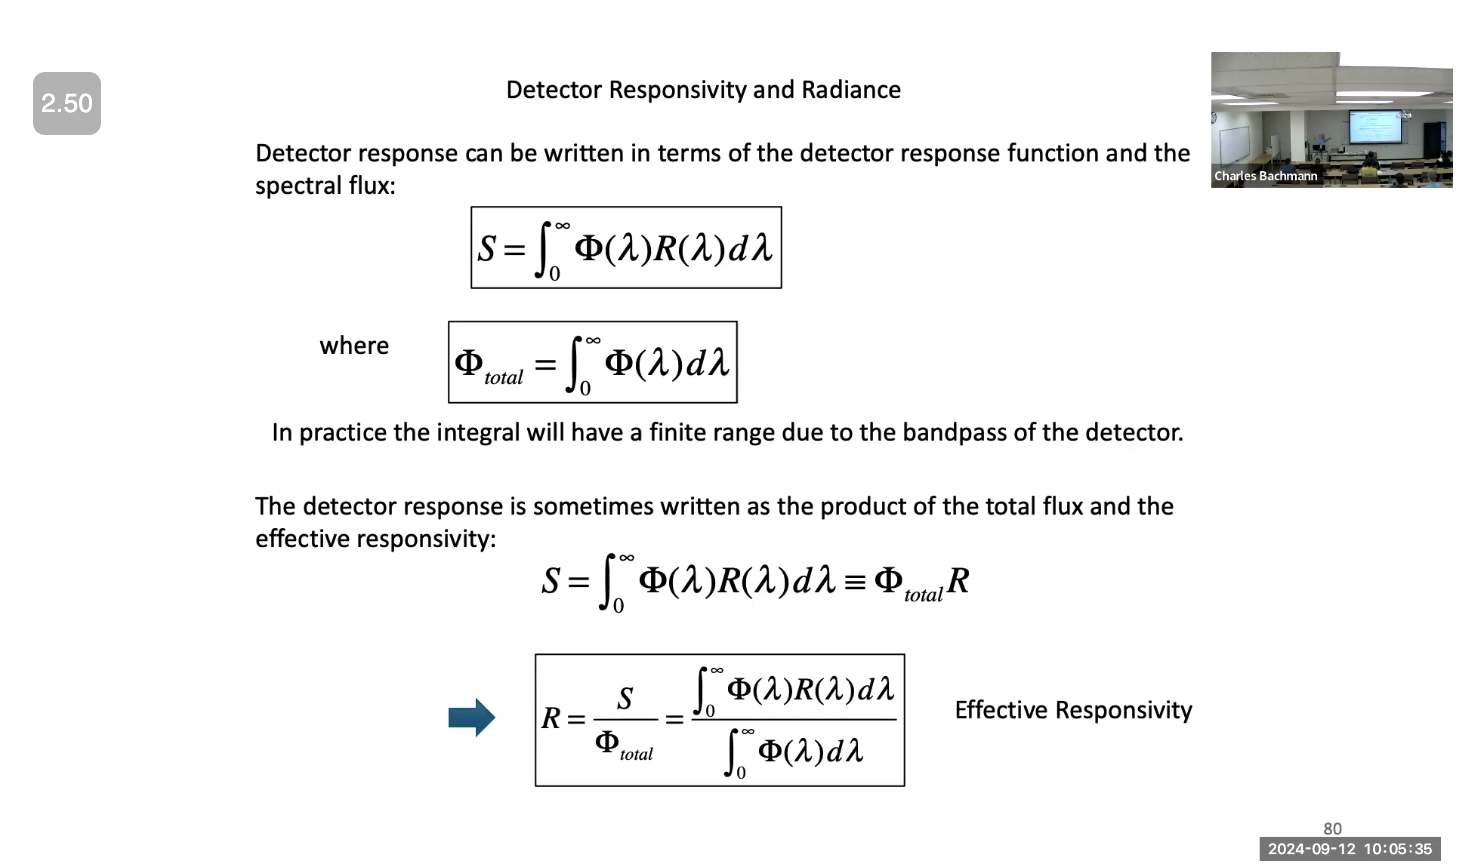
\includegraphics[scale=.6]{Radiometry/Week3/Notes/Sept12Responsivity.png}
\caption{Nugget the Snowman}
\label{fig:Sept Responsivity}
\end{figure}

\begin{figure}[h!]
\centering
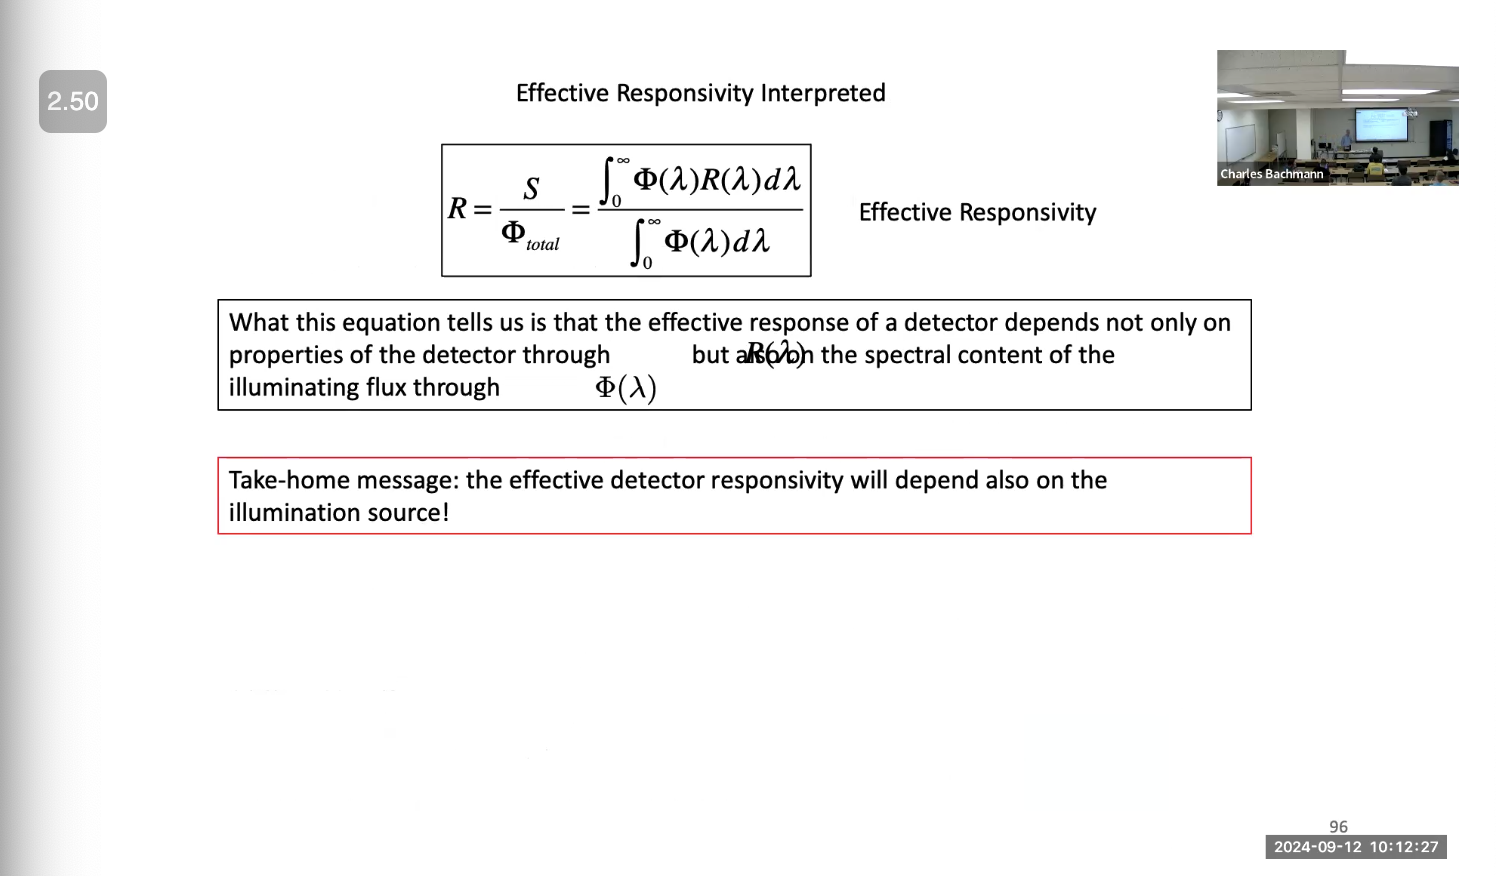
\includegraphics[scale=.6]{Radiometry/Week3/Notes/LightSourceResponsivity.png}
\caption{Nugget the Snowman}
\label{fig:Light Source Responsivity}
\end{figure}


\begin{figure}[h!]
\centering
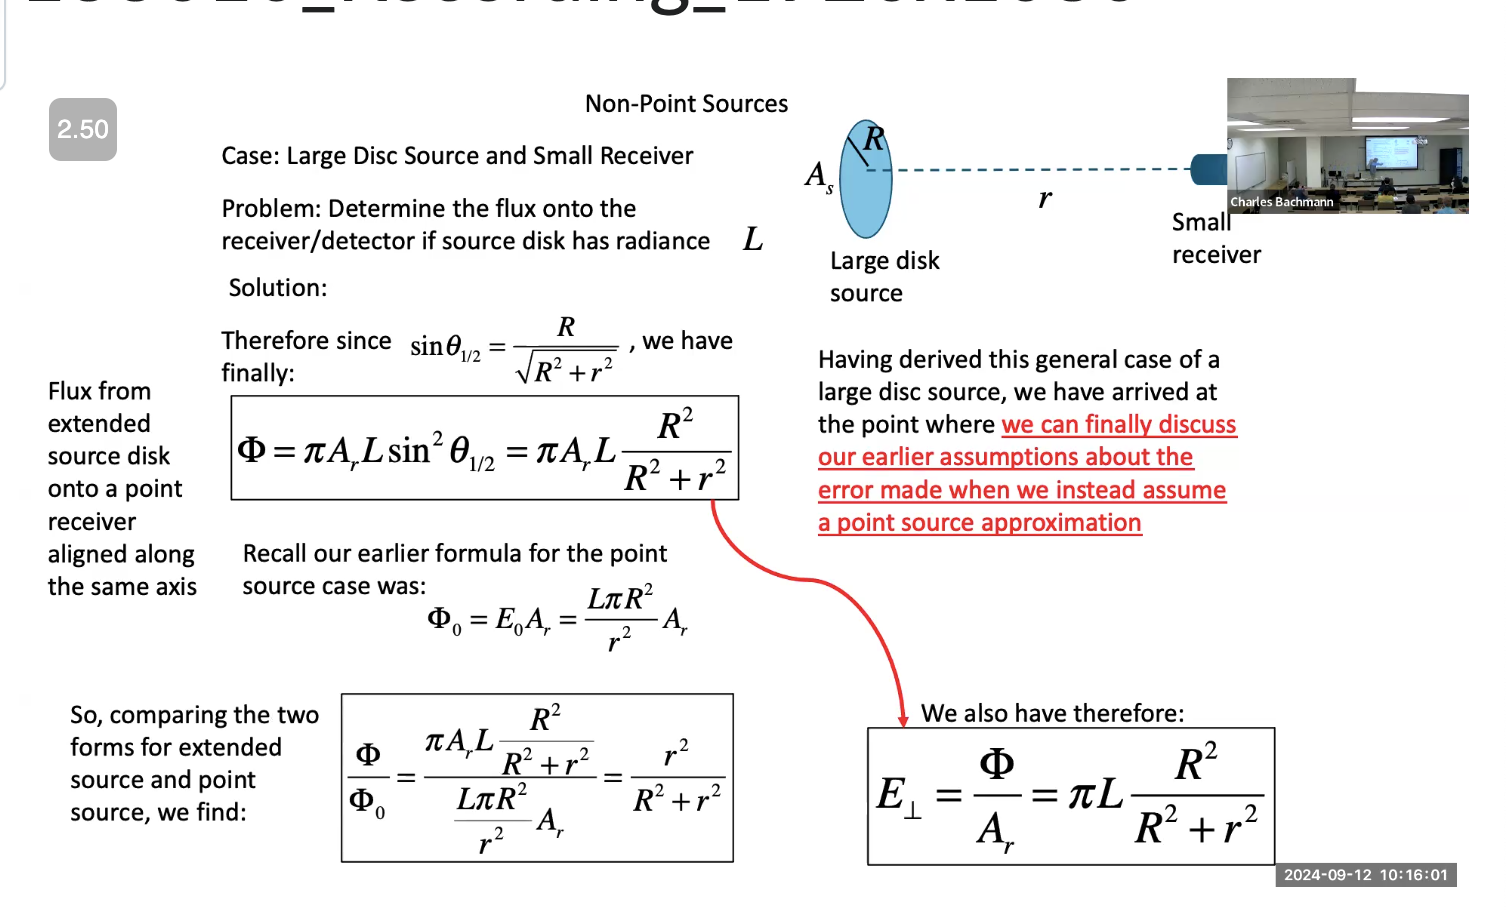
\includegraphics[scale=.6]{Radiometry/Week3/Notes/Mainpoint.png}
\caption{Nugget the Snowman}
\label{fig:Light Source Responsivity}
\end{figure}
\clearpage

\subsection{September 17th, 2024}

Review: Point Source vs. Extended Source 
\begin{figure}[h!]
\centering
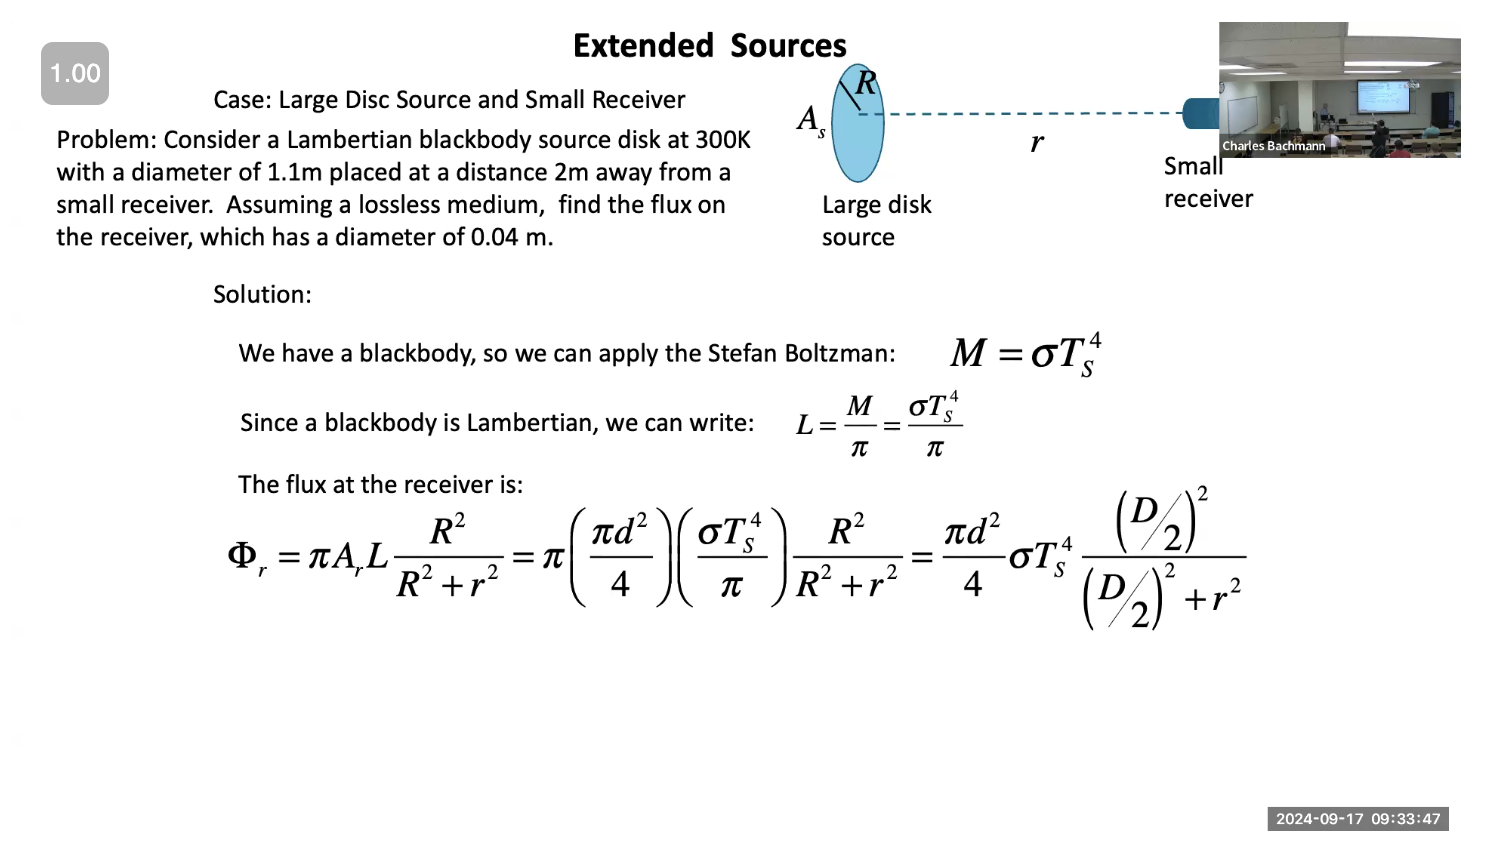
\includegraphics[scale=.6]{Radiometry/Week4/Notes/Sept17/SimpleExtendedSource.png}
\caption{Nugget the Snowman}
\label{fig:Simple Extended Source}
\end{figure}


\begin{figure}[h!]
\centering
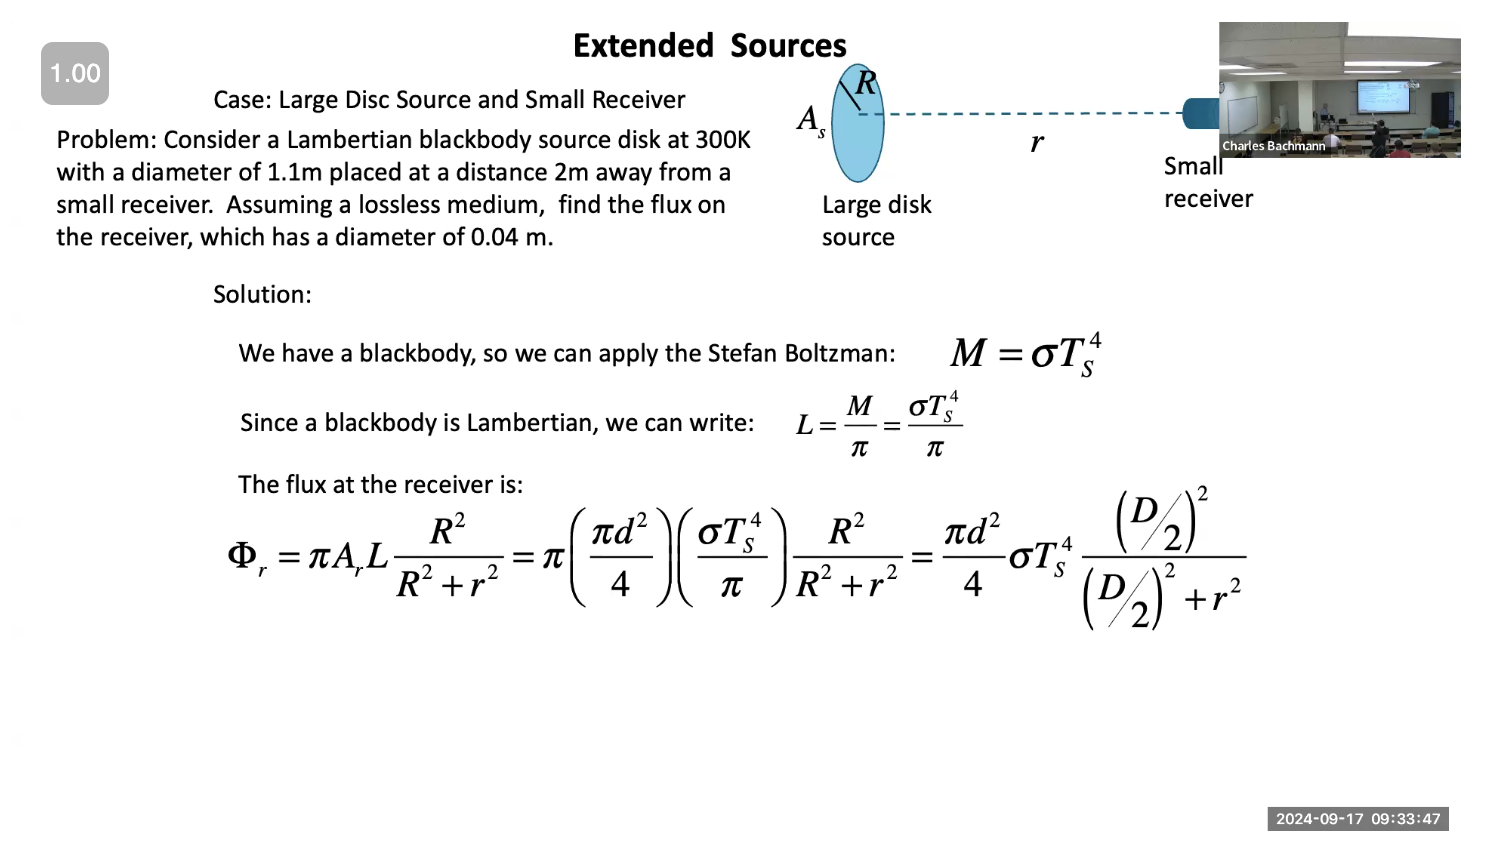
\includegraphics[scale=.6]{Radiometry/Week4/Notes/Sept17/SimpleExtendedSource.png}
\caption{Nugget the Snowman}
\label{fig:Simple Extended Source}
\end{figure}



\clearpage 

More complicated example 


\begin{figure}[h!]
\centering
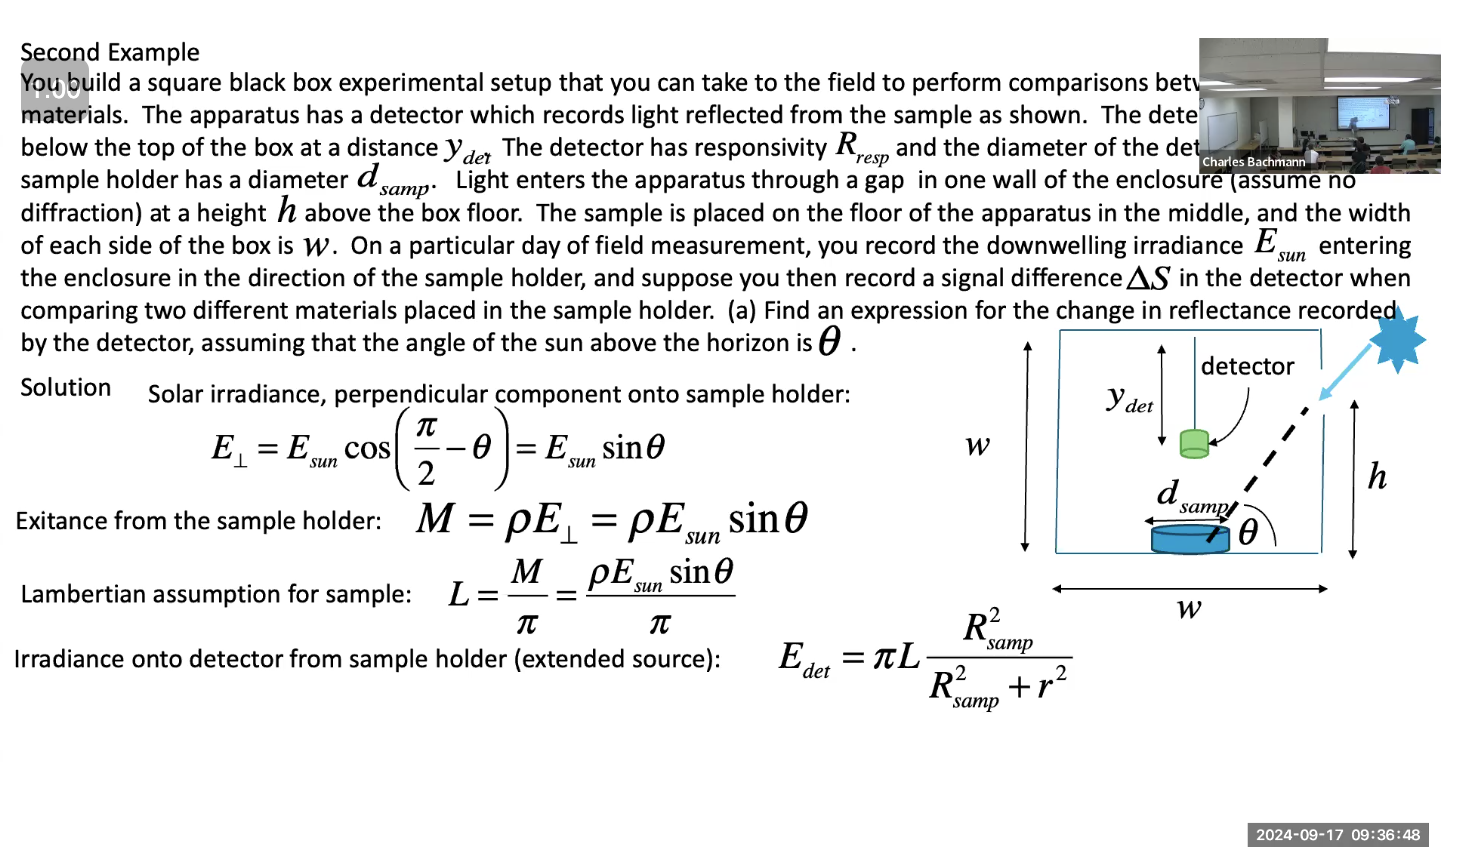
\includegraphics[scale=.6]{Radiometry/Week4/Notes/Sept17/Second.png}
\caption{Nugget the Snowman}
\label{fig:Simple Extended Source}
\end{figure}



\begin{figure}[h!]
\centering
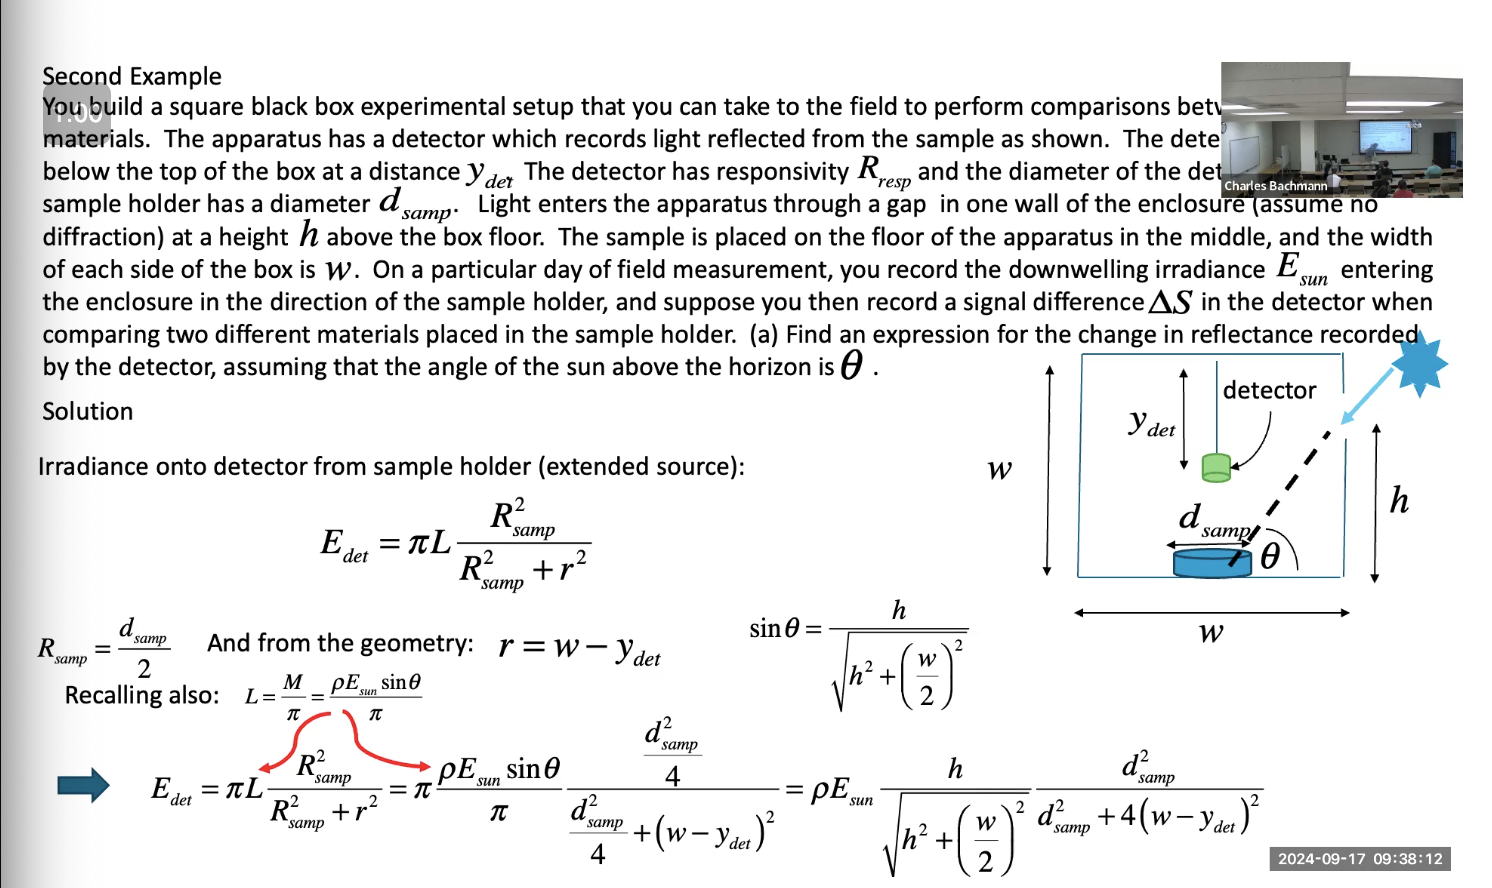
\includegraphics[scale=.6]{Radiometry/Week4/Notes/Sept17/Third.png}
\caption{Nugget the Snowman}
\label{fig:Second}
\end{figure}


\begin{figure}[h!]
\centering
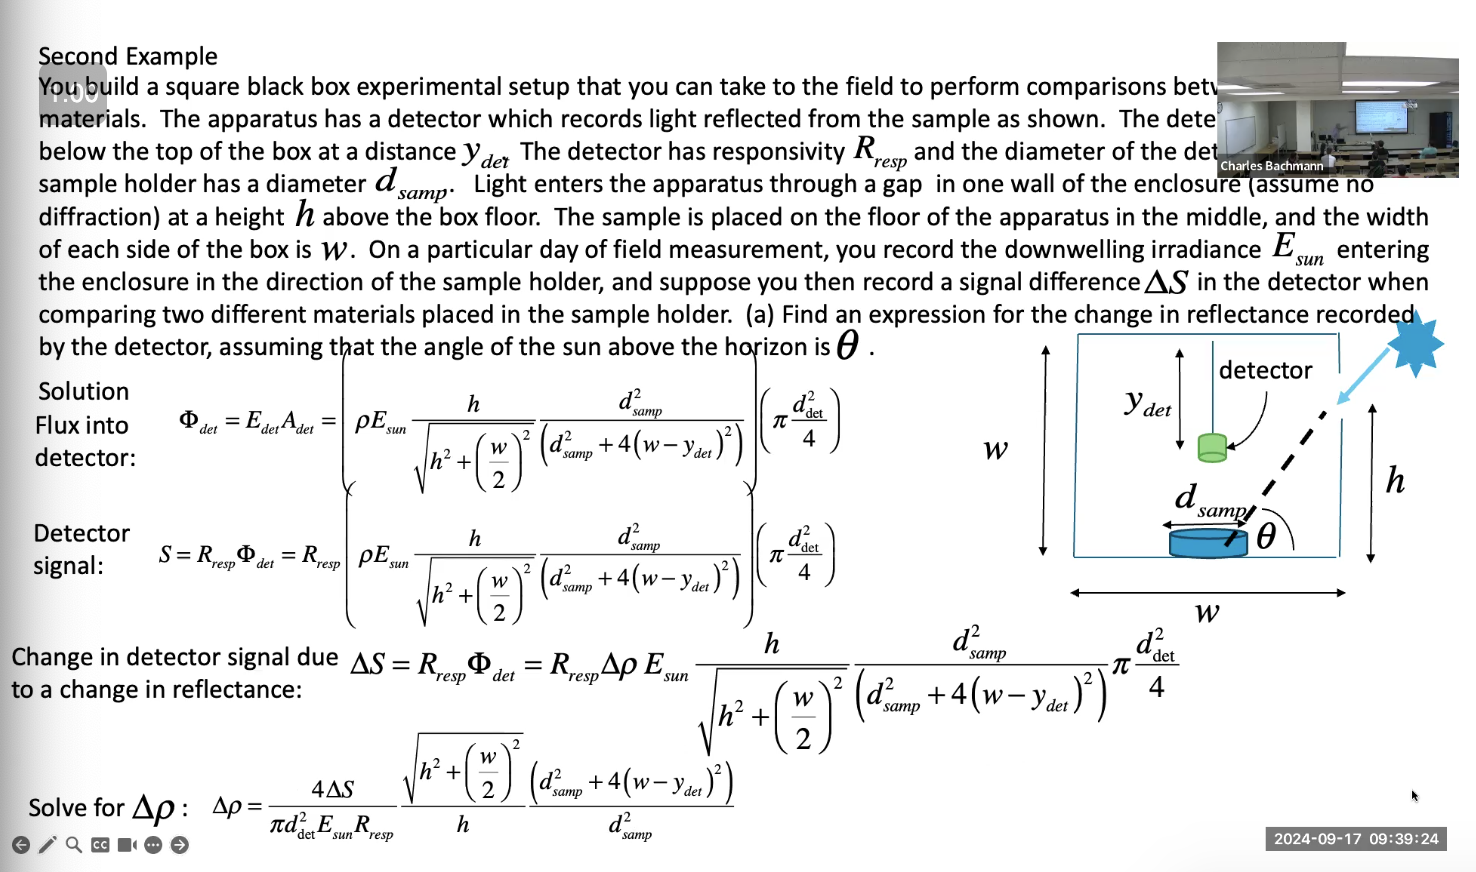
\includegraphics[scale=.6]{Radiometry/Week4/Notes/Sept17/Fourth.png}
\caption{Nugget the Snowman}
\label{fig:Second}
\end{figure}



\begin{figure}[h!]
\centering
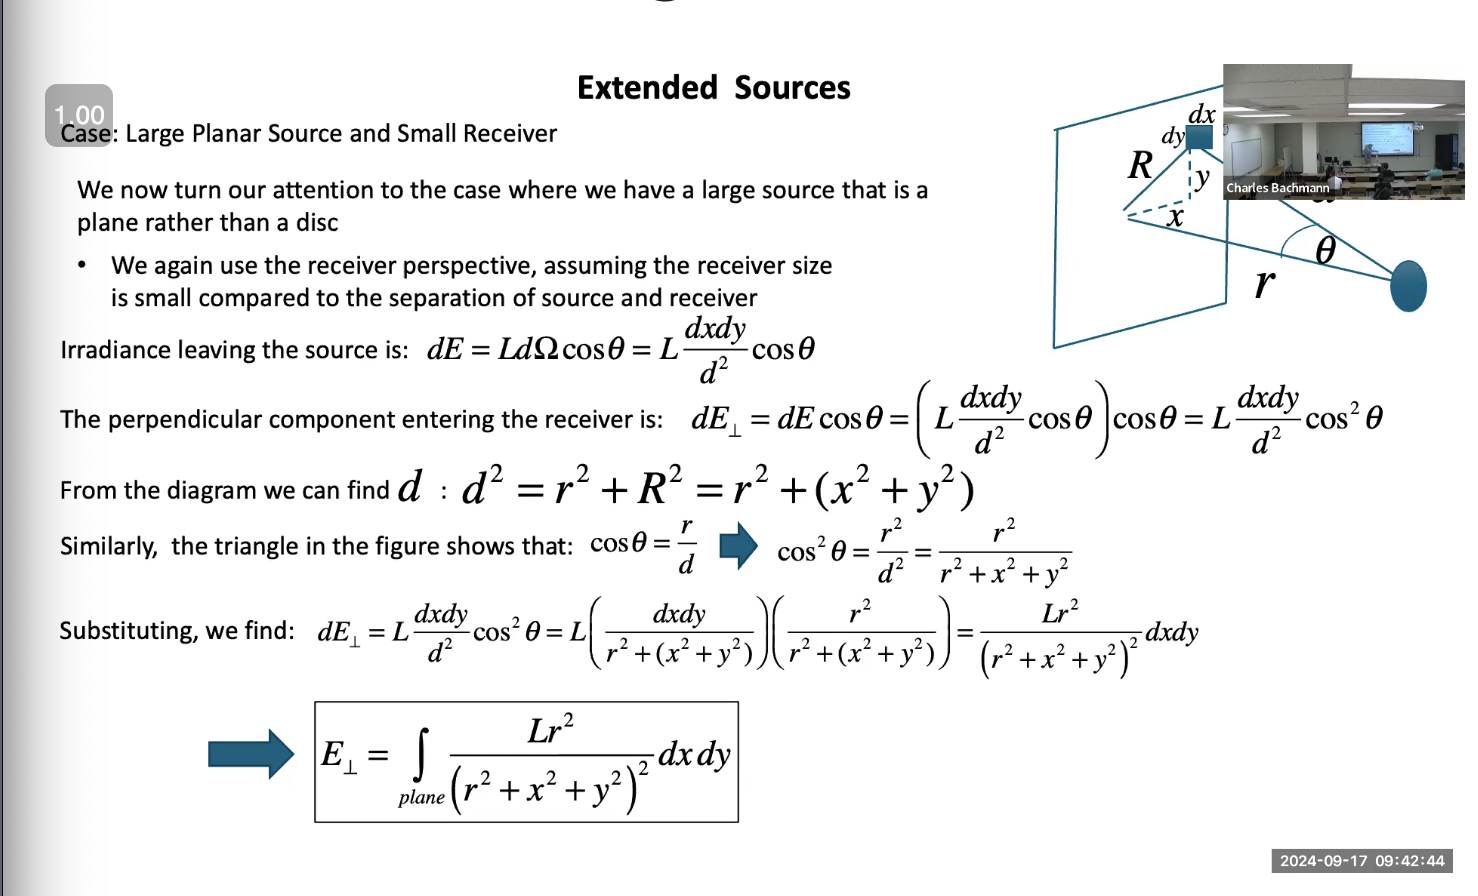
\includegraphics[scale=.6]{Radiometry/Week4/Notes/Sept17/Plane.png}
\caption{Nugget the Snowman}
\label{fig:Plane}
\end{figure}


\begin{figure}[h!]
\centering
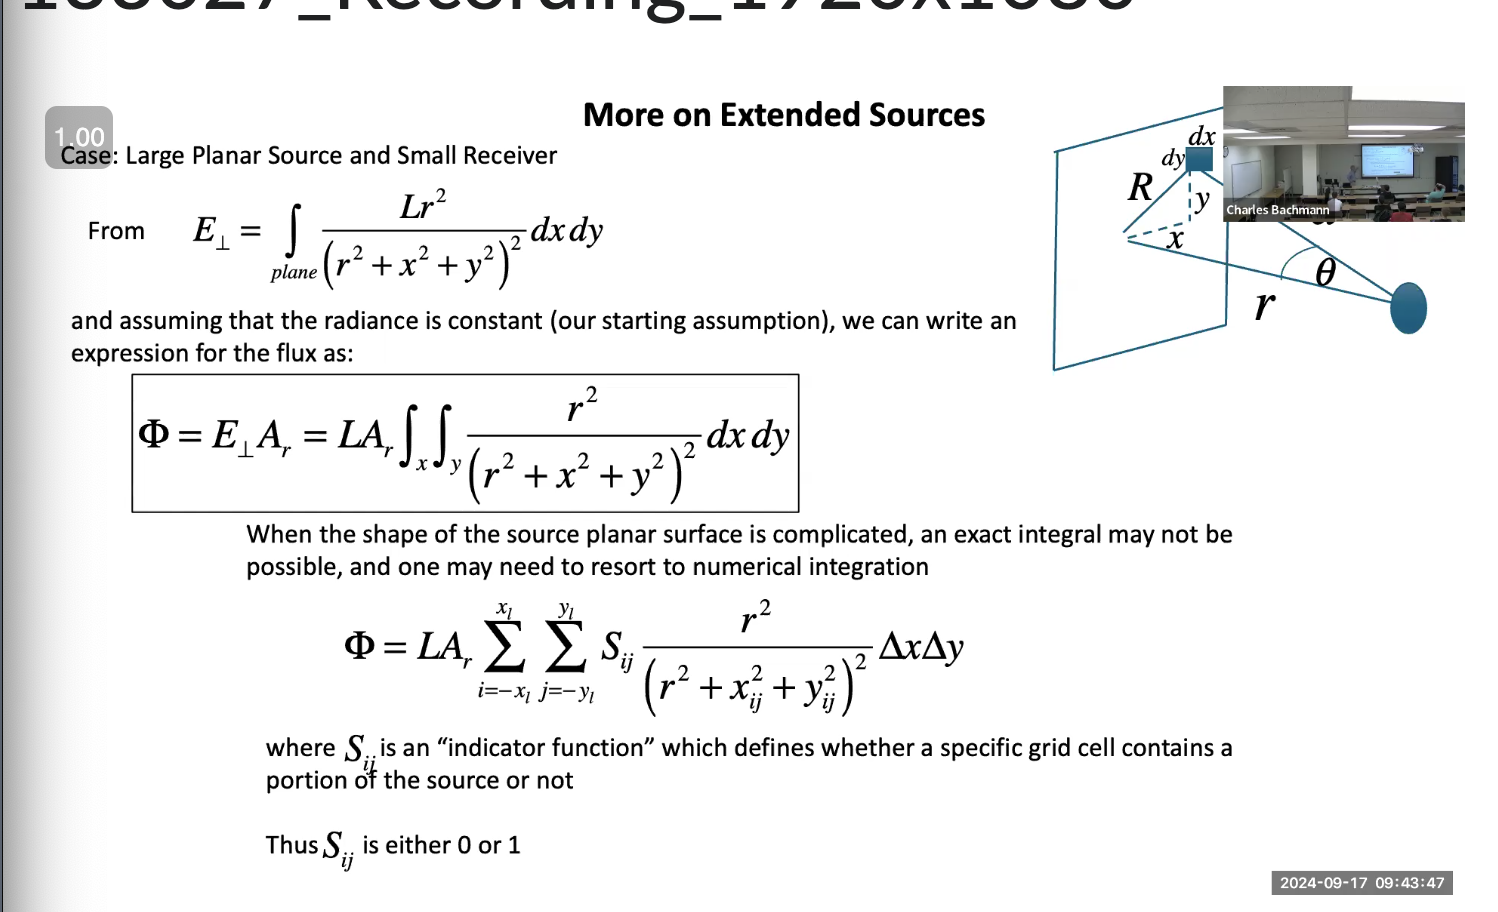
\includegraphics[scale=.6]{Radiometry/Week4/Notes/Sept17/Plane2.png}
\caption{Nugget the Snowman}
\label{fig:Plane2}
\end{figure}

\begin{figure}[h!]
\centering
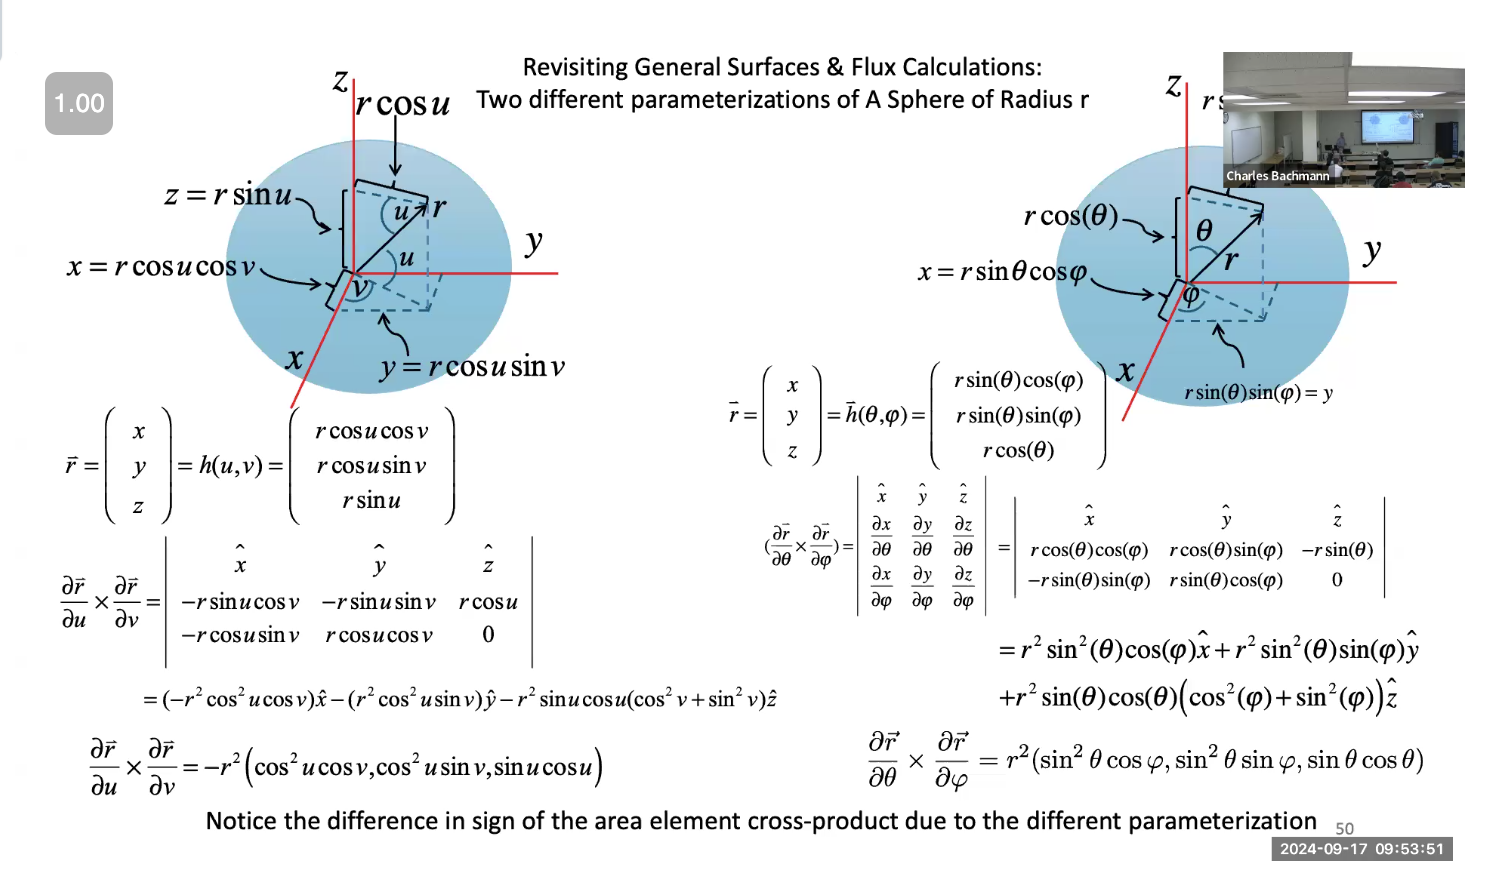
\includegraphics[scale=.6]{Radiometry/Week4/Notes/Sept17/Spherical.png}
\caption{Nugget the Snowman}
\label{fig:Spherical}
\end{figure}


\begin{figure}[h!]
\centering
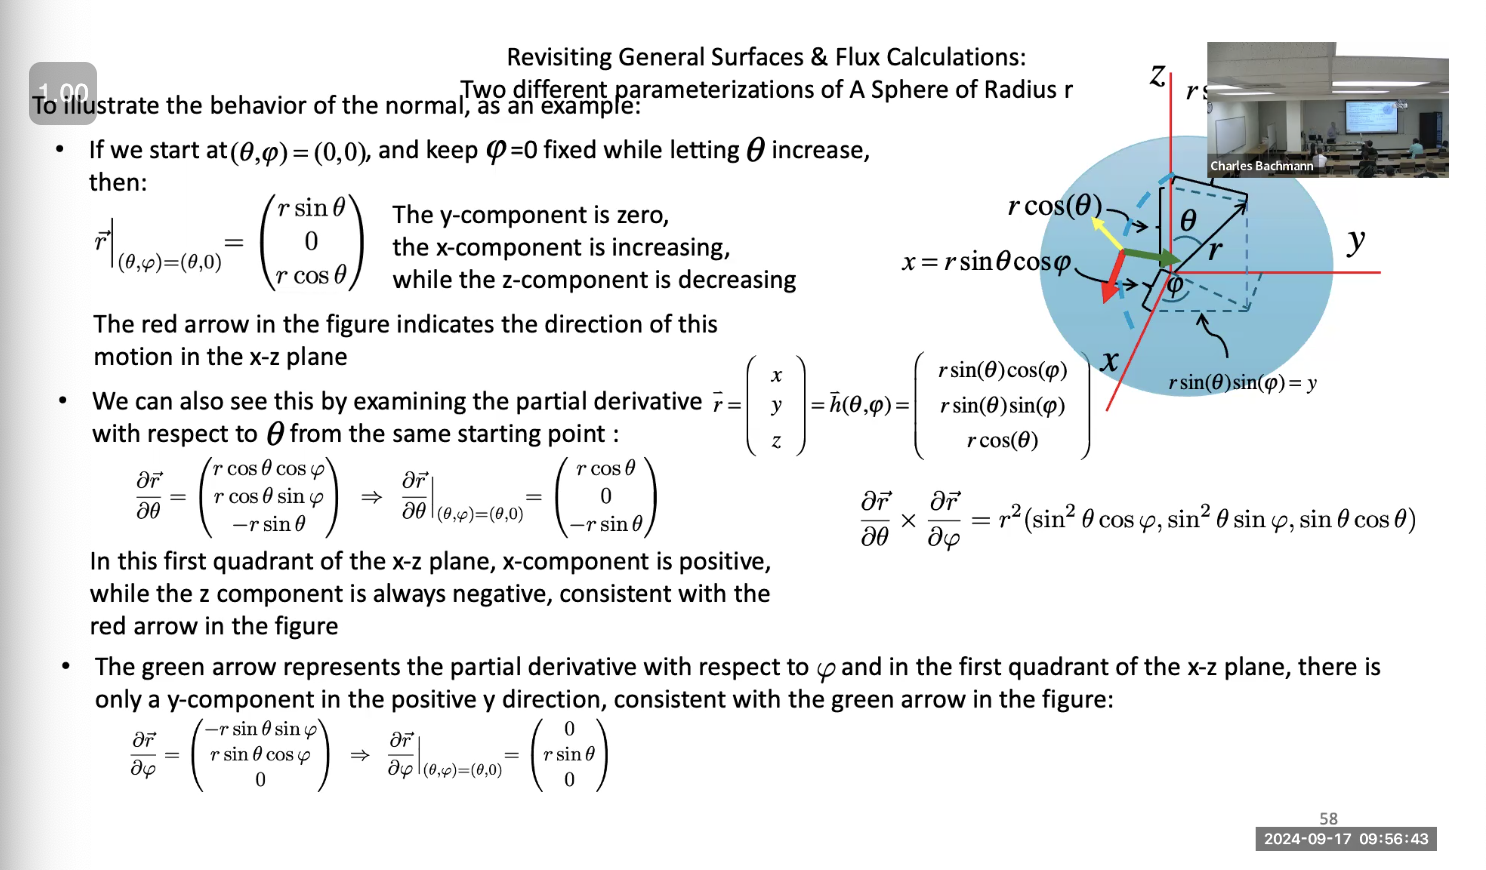
\includegraphics[scale=.6]{Radiometry/Week4/Notes/Sept17/Spherical2.png}
\caption{Nugget the Snowman}
\label{fig:Spherical2}
\end{figure}

\clearpage
\subsubsection{ERROR PROPAGATION}

\begin{figure}[h!]
\centering
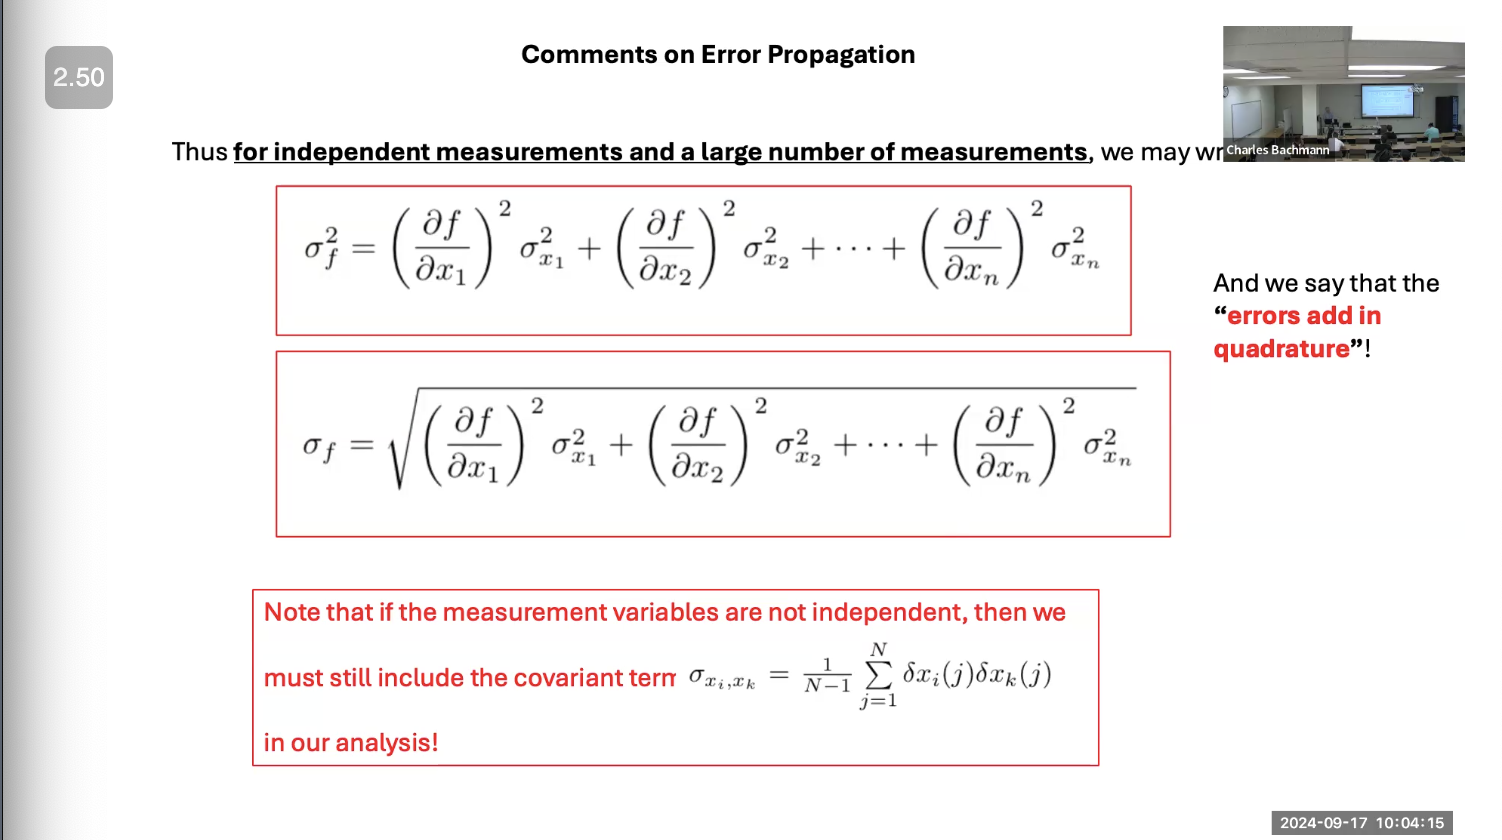
\includegraphics[scale=.6]{Radiometry/Week4/Notes/Sept17/Quadrature2.png}
\caption{Nugget the Snowman}
\label{fig:Quadrature2}
\end{figure}


\begin{figure}[h!]
\centering
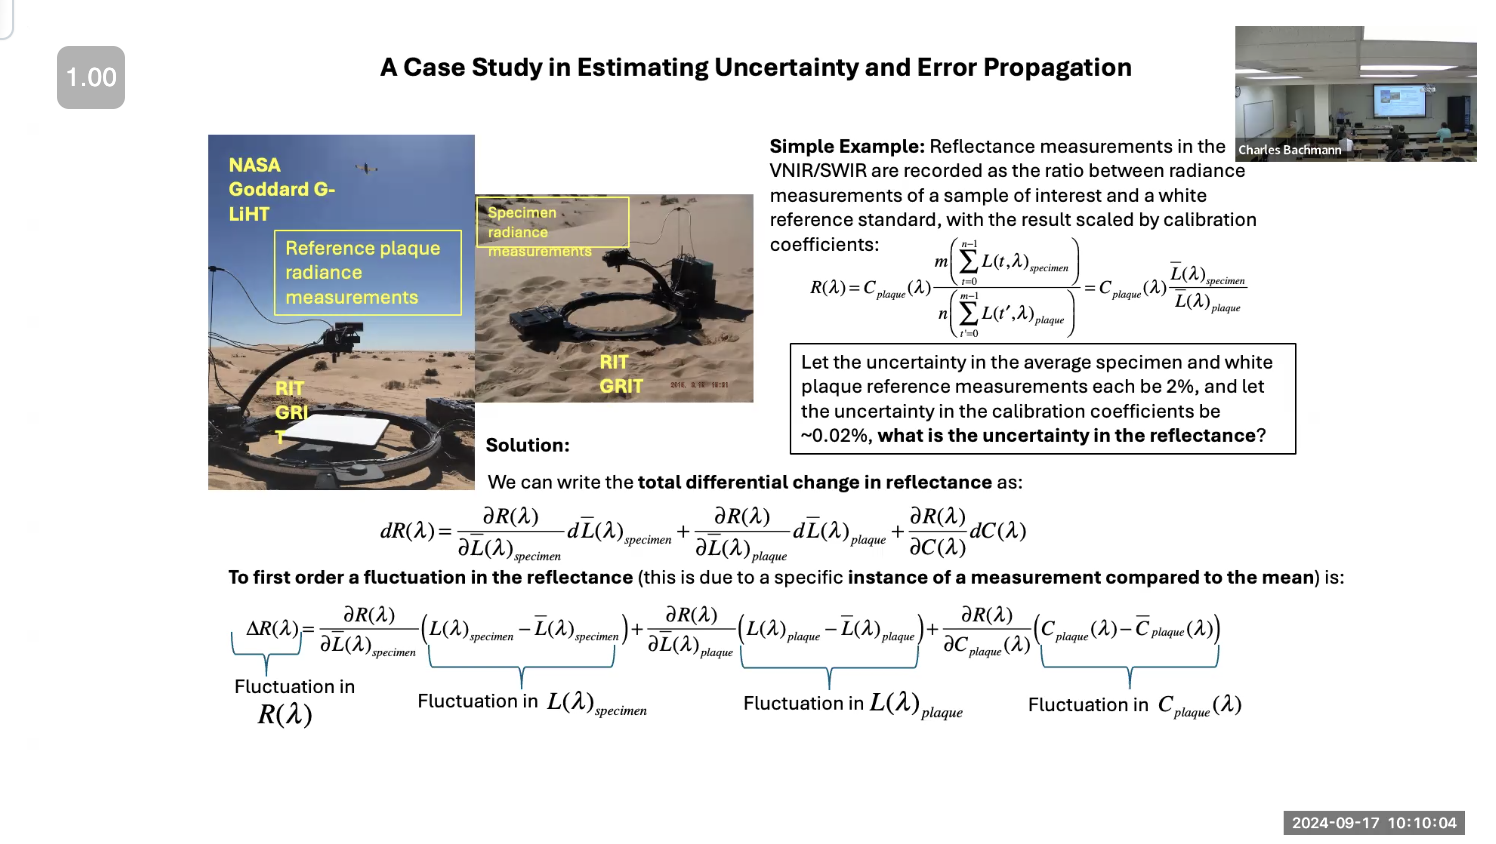
\includegraphics[scale=.6]{Radiometry/Week4/Notes/Sept17/Goiniometer.png}
\caption{Nugget the Snowman}
\label{fig:Goiniometer}
\end{figure}


\begin{figure}[h!]
\centering
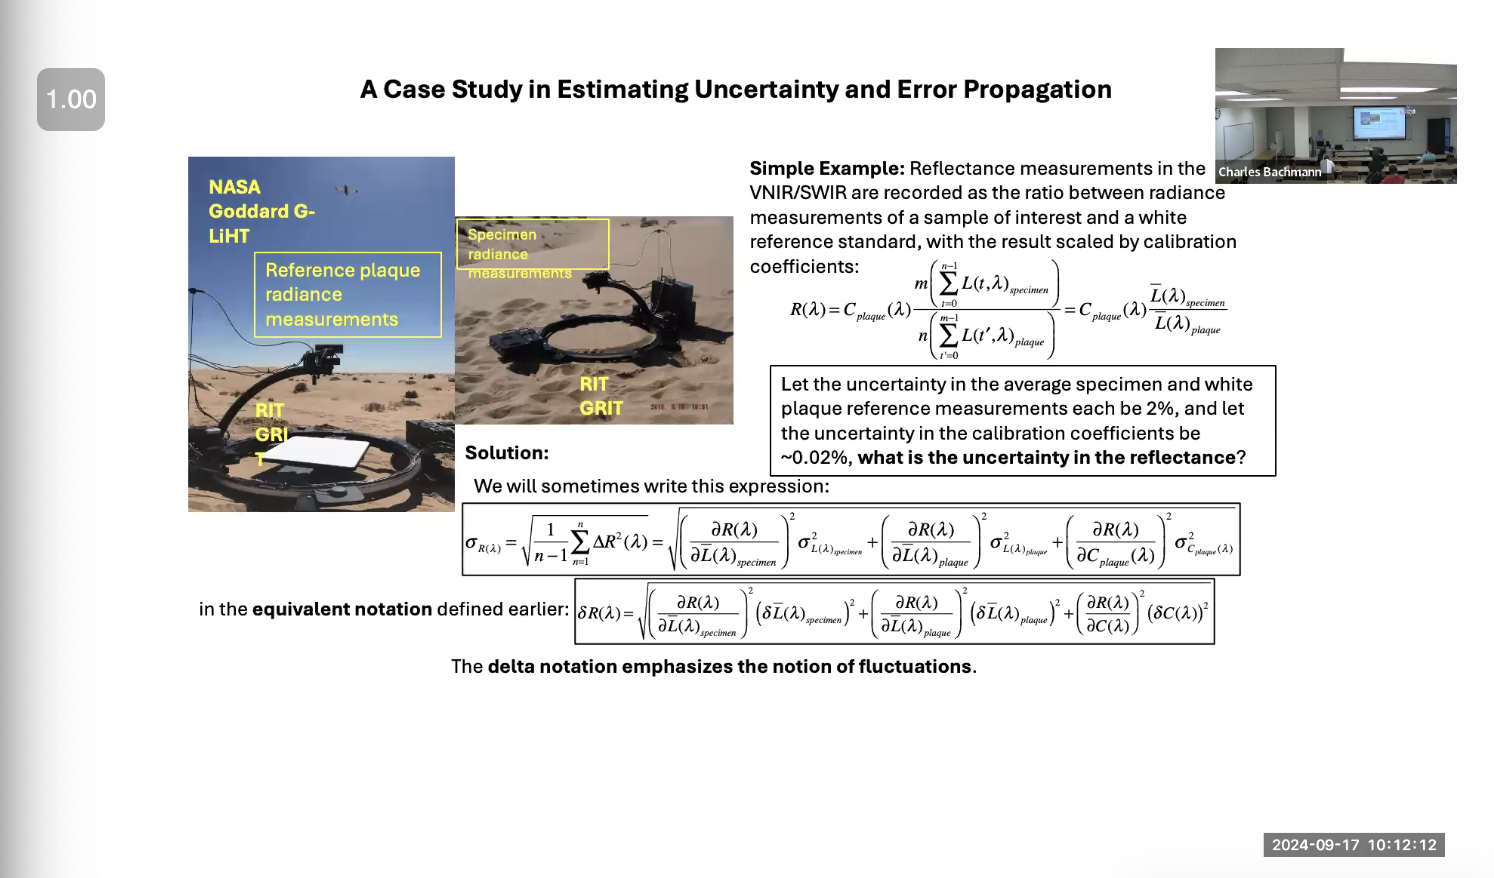
\includegraphics[scale=.6]{Radiometry/Week4/Notes/Sept17/Goiniometer2.png}
\caption{Nugget the Snowman}
\label{fig:Goiniometer2}
\end{figure}
\clearpage

\begin{figure}[h!]
\centering
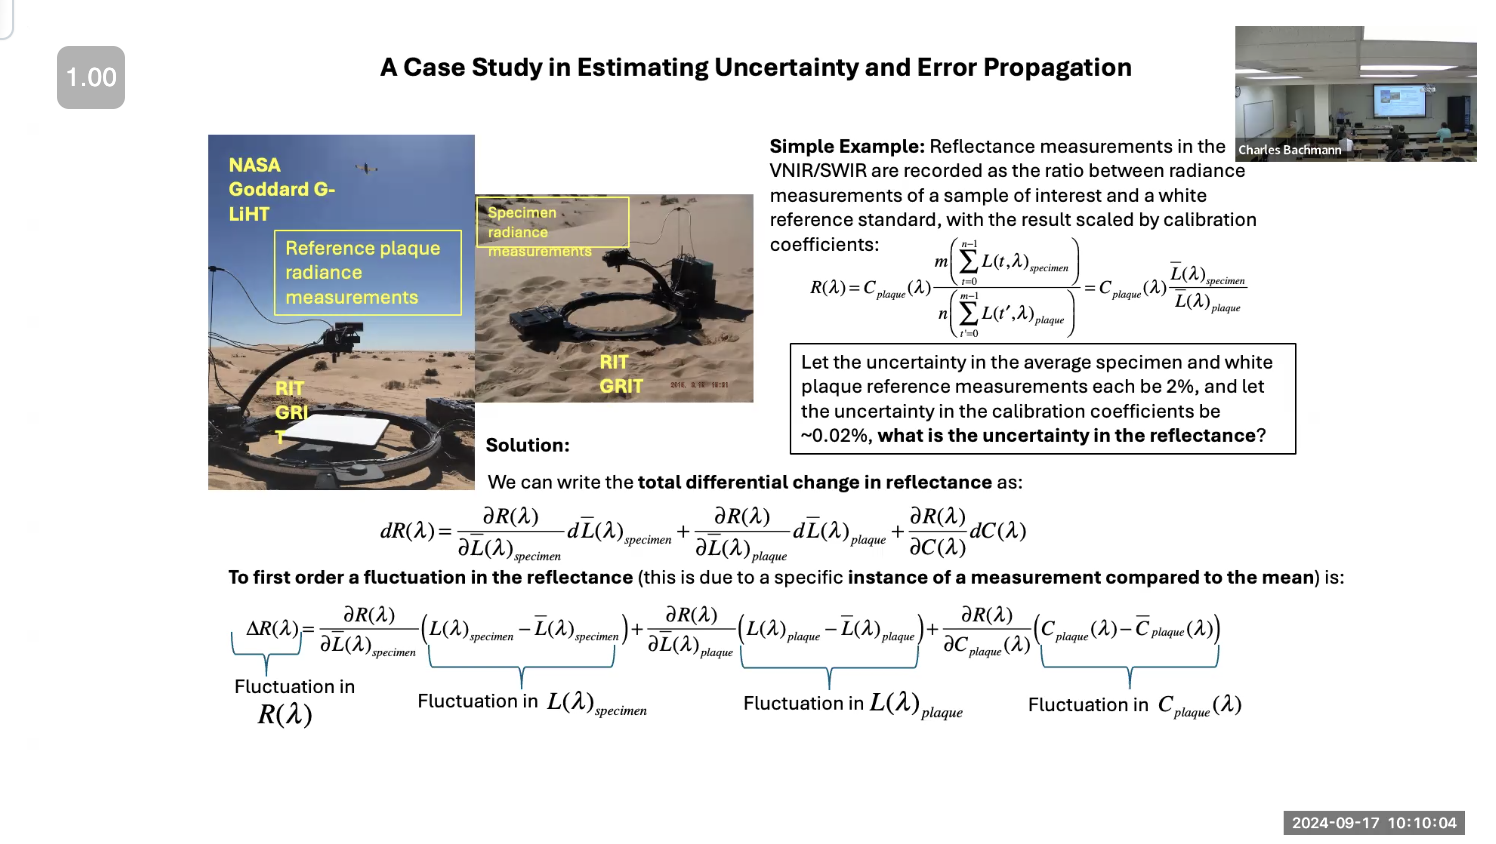
\includegraphics[scale=.6]{Radiometry/Week4/Notes/Sept17/Goiniometer.png}
\caption{Nugget the Snowman}
\label{fig:Goiniometer}
\end{figure}
\clearpage

\subsubsection{Blackbody}


\begin{figure}[h!]
\centering
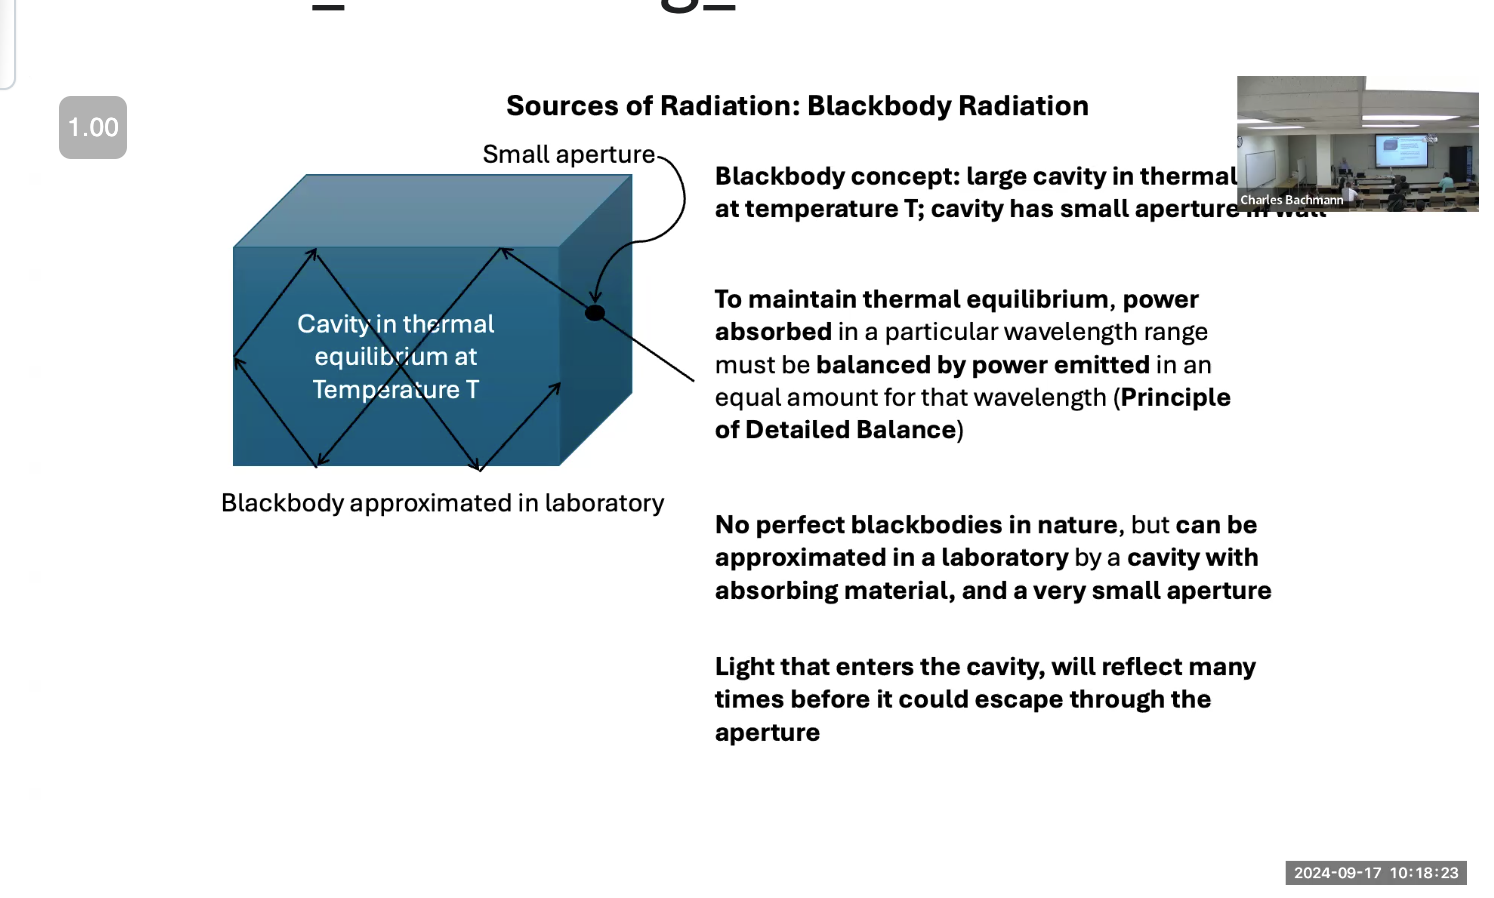
\includegraphics[scale=.6]{Radiometry/Week4/Notes/Sept17/Blackbody.png}
\caption{Nugget the Snowman}
\label{fig:Blackbody}
\end{figure}

\begin{figure}[h!]
\centering
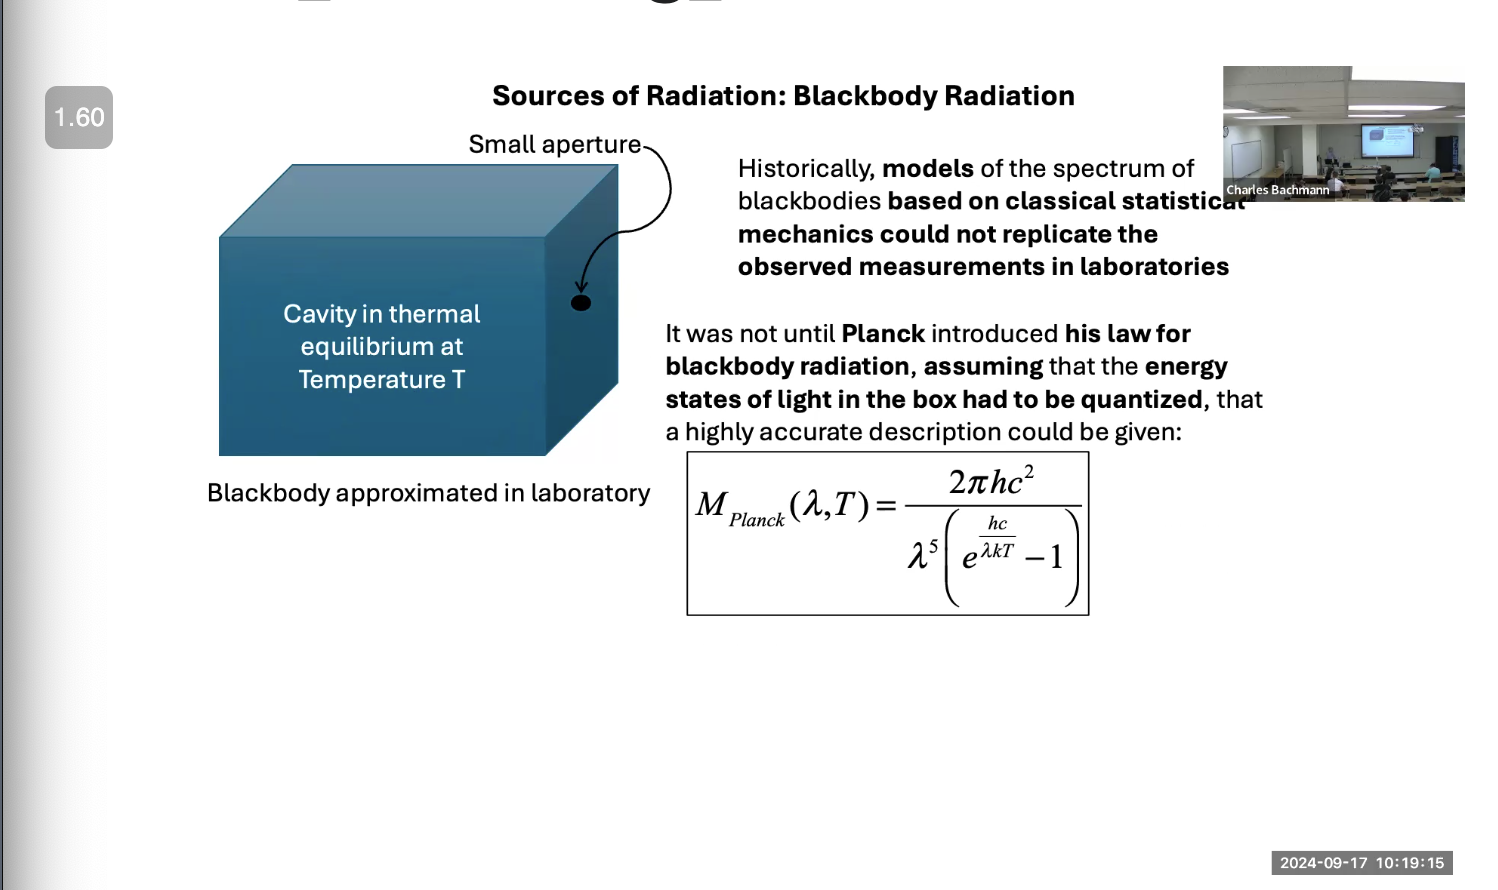
\includegraphics[scale=.6]{Radiometry/Week4/Notes/Sept17/Blackbody2.png}
\caption{Nugget the Snowman}
\label{fig:Blackbody2}
\end{figure}
\clearpage

\subsection{PSET 2 Review September 19th, 2024}

\subsubsection{Problem 1}
\begin{figure}[h!]
\centering
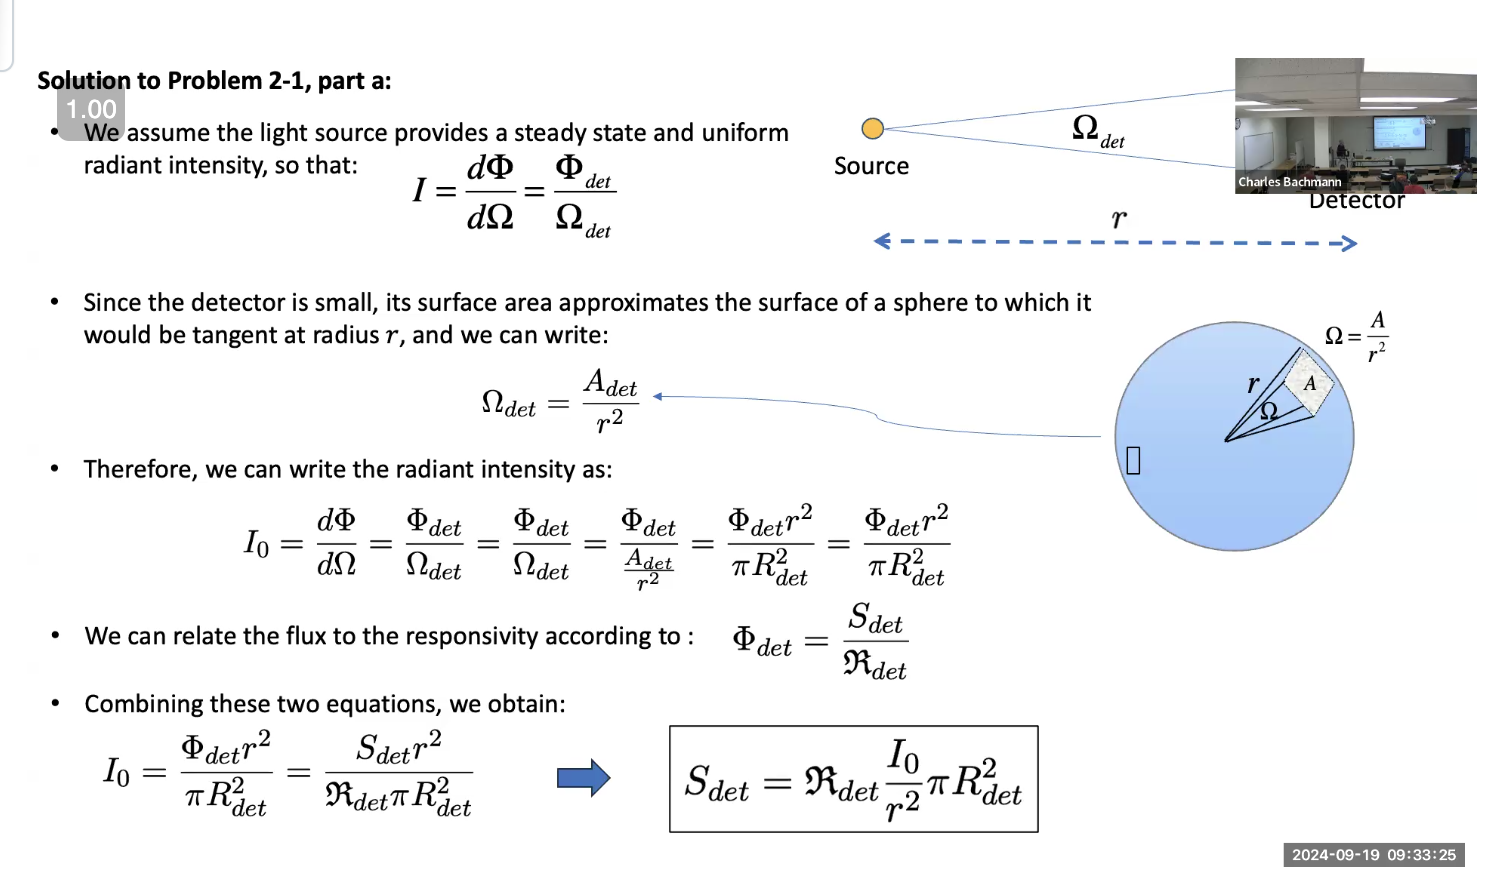
\includegraphics[scale=.6]{Radiometry/Week4/Notes/PSET2/P1.png}
\caption{Nugget the Snowman}
\label{fig:P1}
\end{figure}
\subsubsection{Problem 2: DIFFUSER MIDTERM QUESTION AND POSSIBLE EXAM PROBLEM
}

\begin{figure}[h!]
\centering
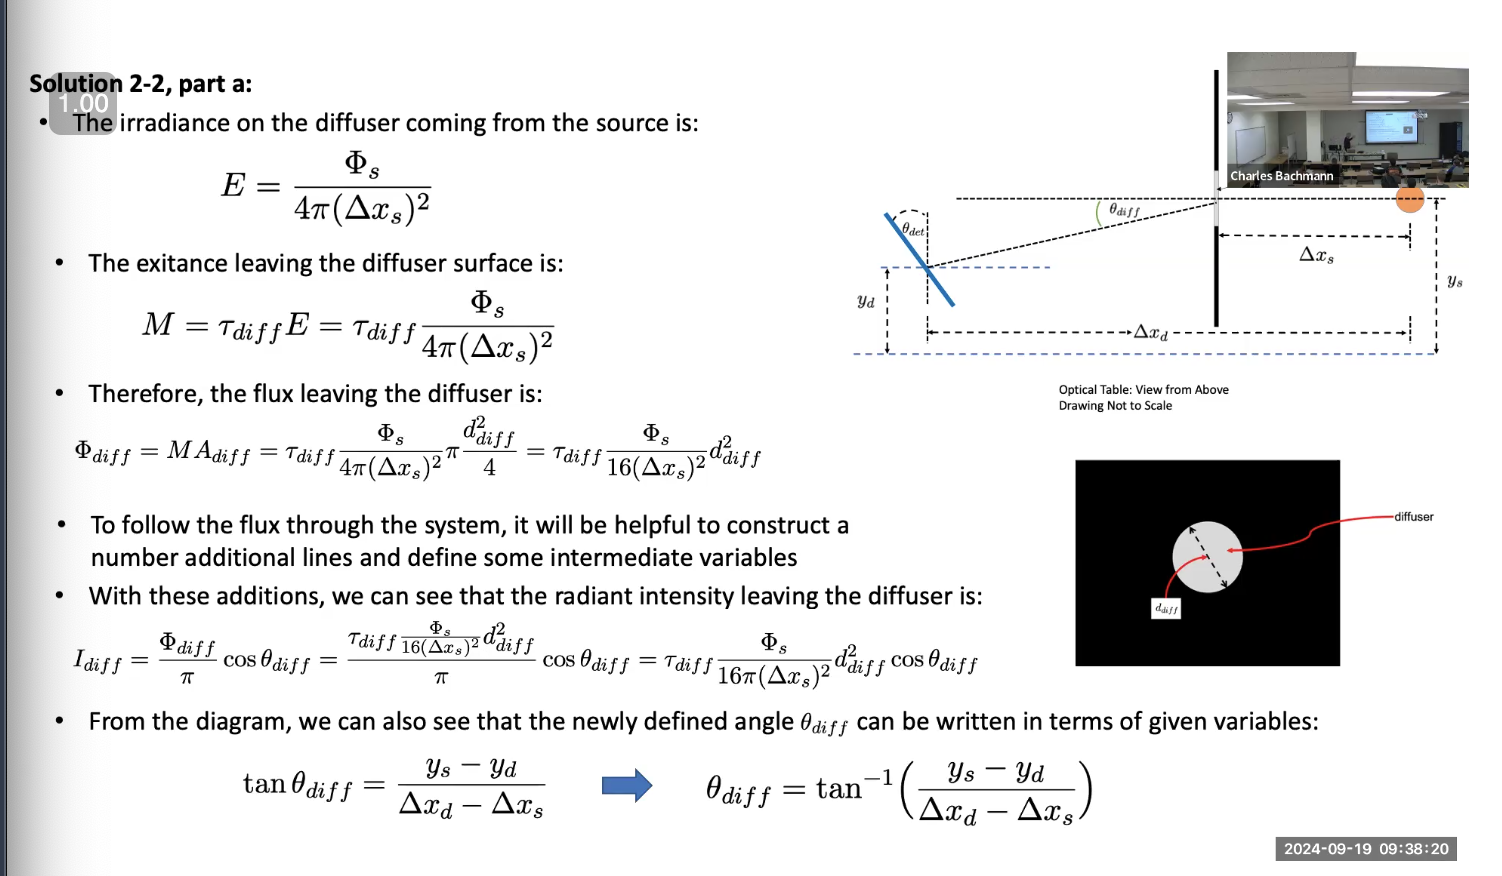
\includegraphics[scale=.6]{Radiometry/Week4/Notes/PSET2/P2.png}
\caption{Nugget the Snowman}
\label{fig:P2}
\end{figure}


\begin{figure}[h!]
\centering
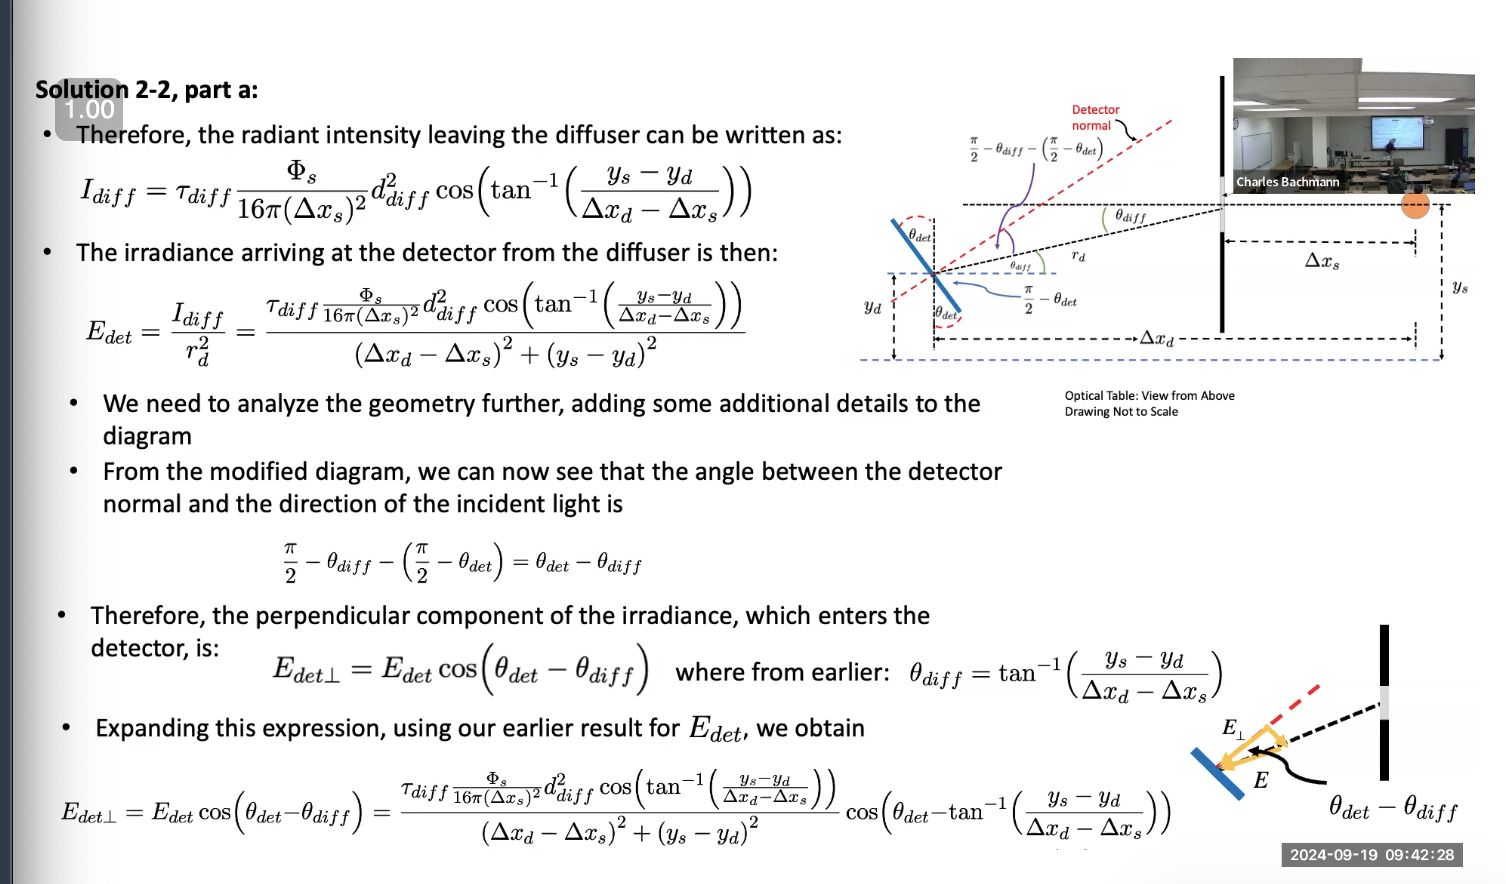
\includegraphics[scale=.6]{Radiometry/Week4/Notes/PSET2/P2a.png}
\caption{Nugget the Snowman}
\label{fig:P2a}
\end{figure}


\begin{figure}[h!]
\centering
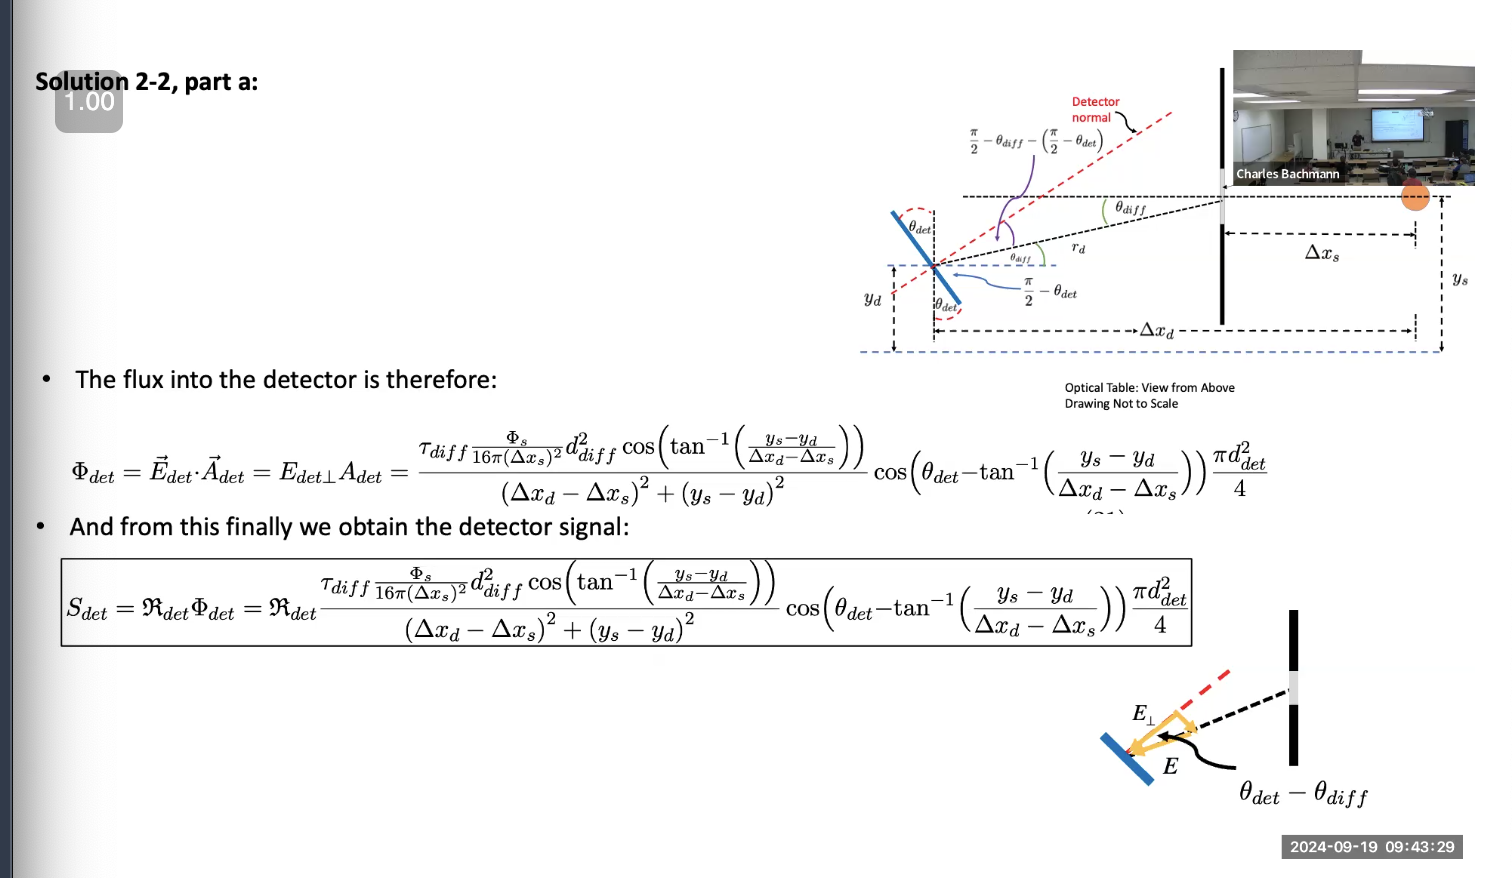
\includegraphics[scale=.6]{Radiometry/Week4/Notes/PSET2/P2aa.png}
\caption{Nugget the Snowman}
\label{fig:P2aa}
\end{figure}

\begin{figure}[h!]
\centering
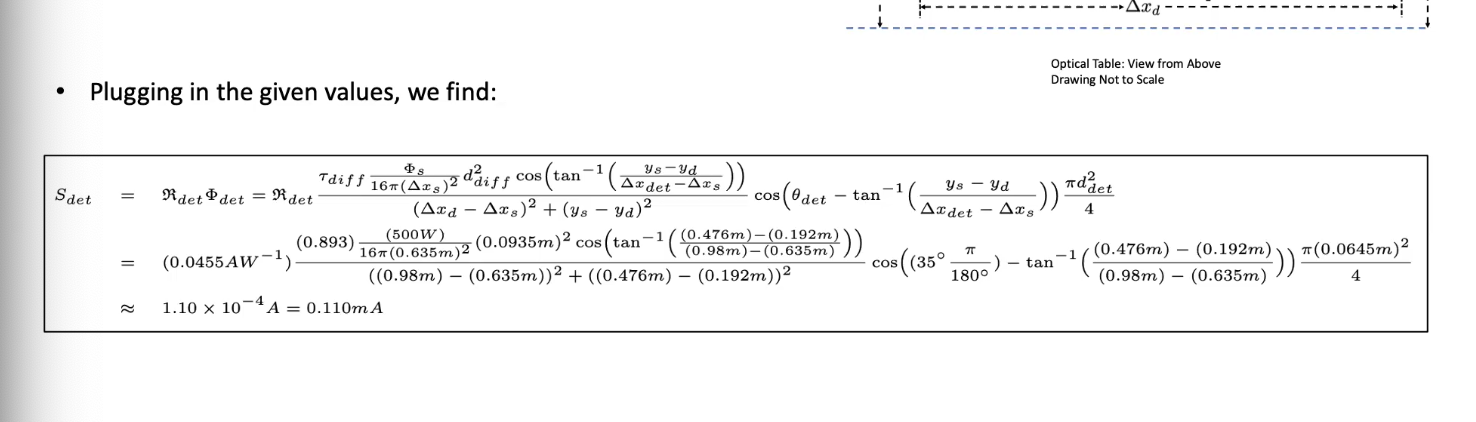
\includegraphics[scale=.6]{Radiometry/Week4/Notes/PSET2/P2aaa.png}
\caption{Nugget the Snowman}
\label{fig:P2aaa}
\end{figure}

\subsubsection{Problem 3: Rotating Stage}
\begin{figure}[h!]
\centering
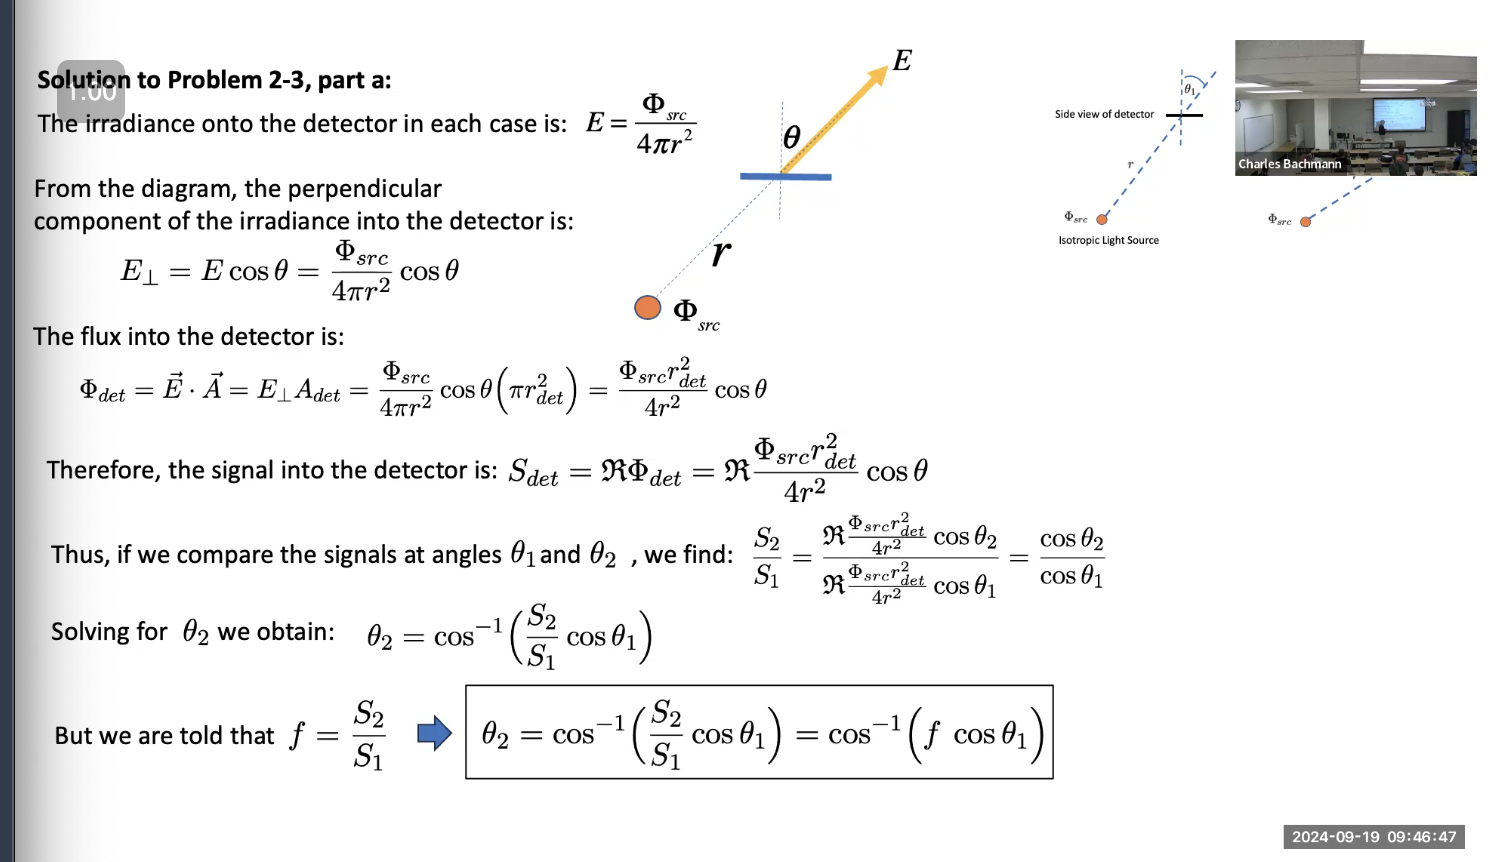
\includegraphics[scale=.6]{Radiometry/Week4/Notes/PSET2/P3/P3.png}
\caption{Nugget the Snowman}
\label{fig:P3}
\end{figure}


\begin{figure}[h!]
\centering
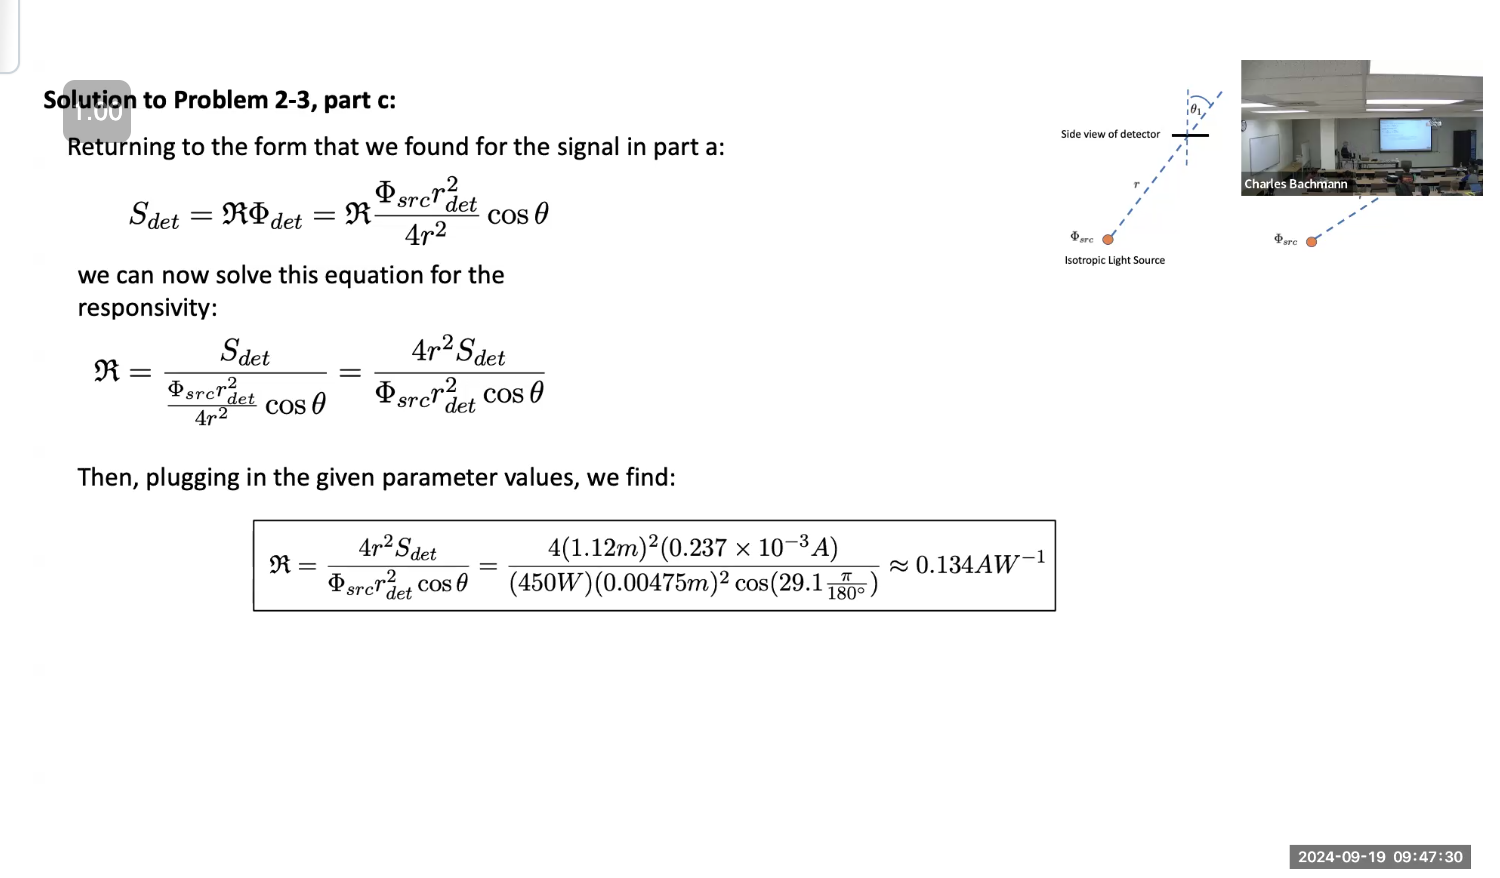
\includegraphics[scale=.6]{Radiometry/Week4/Notes/PSET2/P3/P3c.png}
\caption{Nugget the Snowman}
\label{fig:P3}
\end{figure}

\subsubsection{EXTENDED SOURCES: MIDTERM QUESTION: POSSIBLE FINAL QUESTION}

Need irradiance, normal component, exitance and know that the tile is LAMBERTIAN

\begin{figure}[h!]
\centering
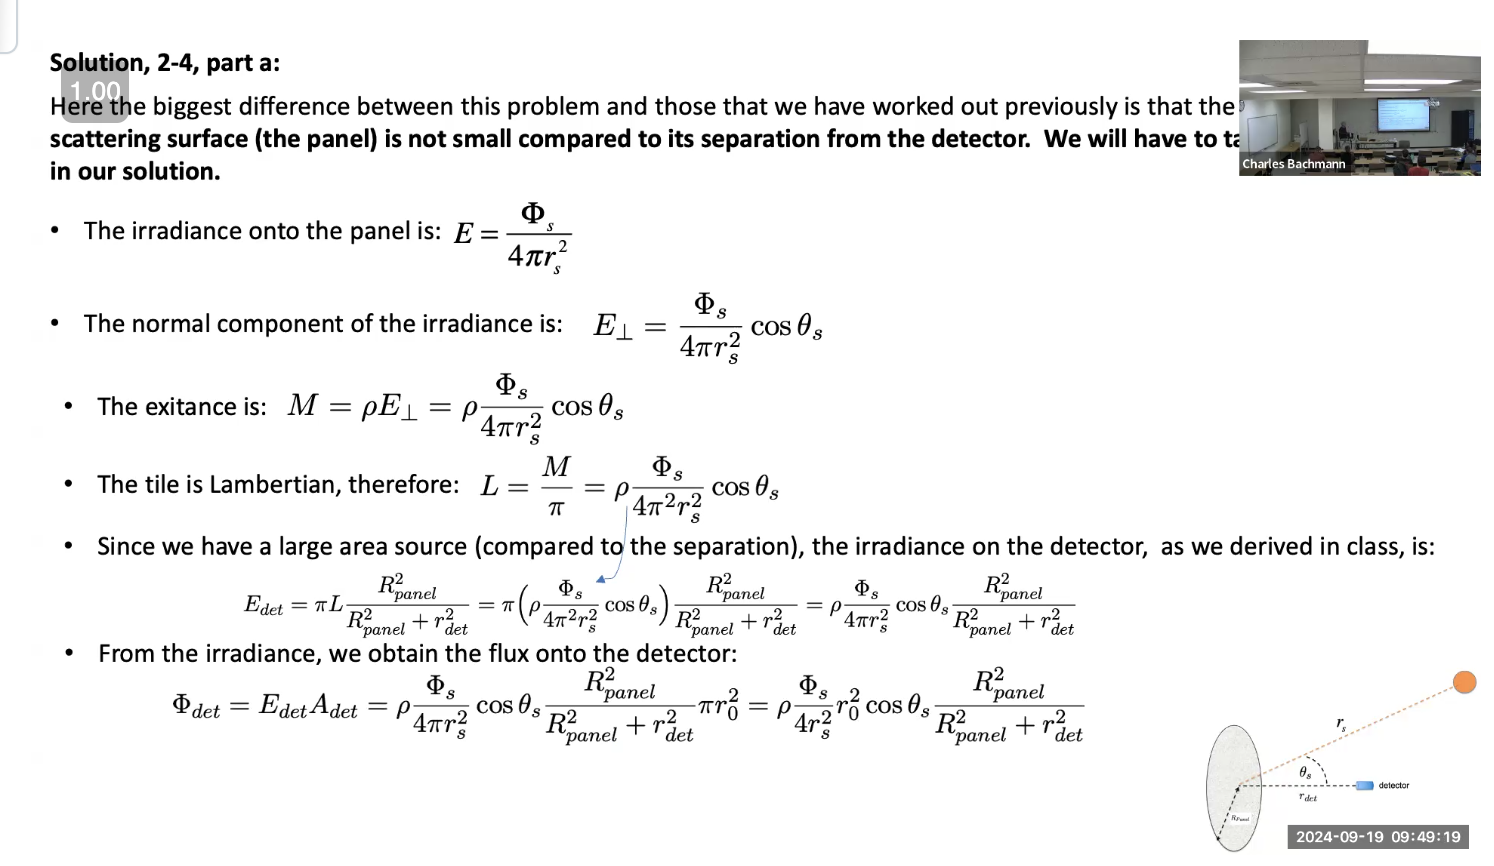
\includegraphics[scale=.6]{Radiometry/Week4/Notes/PSET2/P4/P4.png}
\caption{Nugget the Snowman}
\label{fig:P4}
\end{figure}


\begin{figure}[h!]
\centering
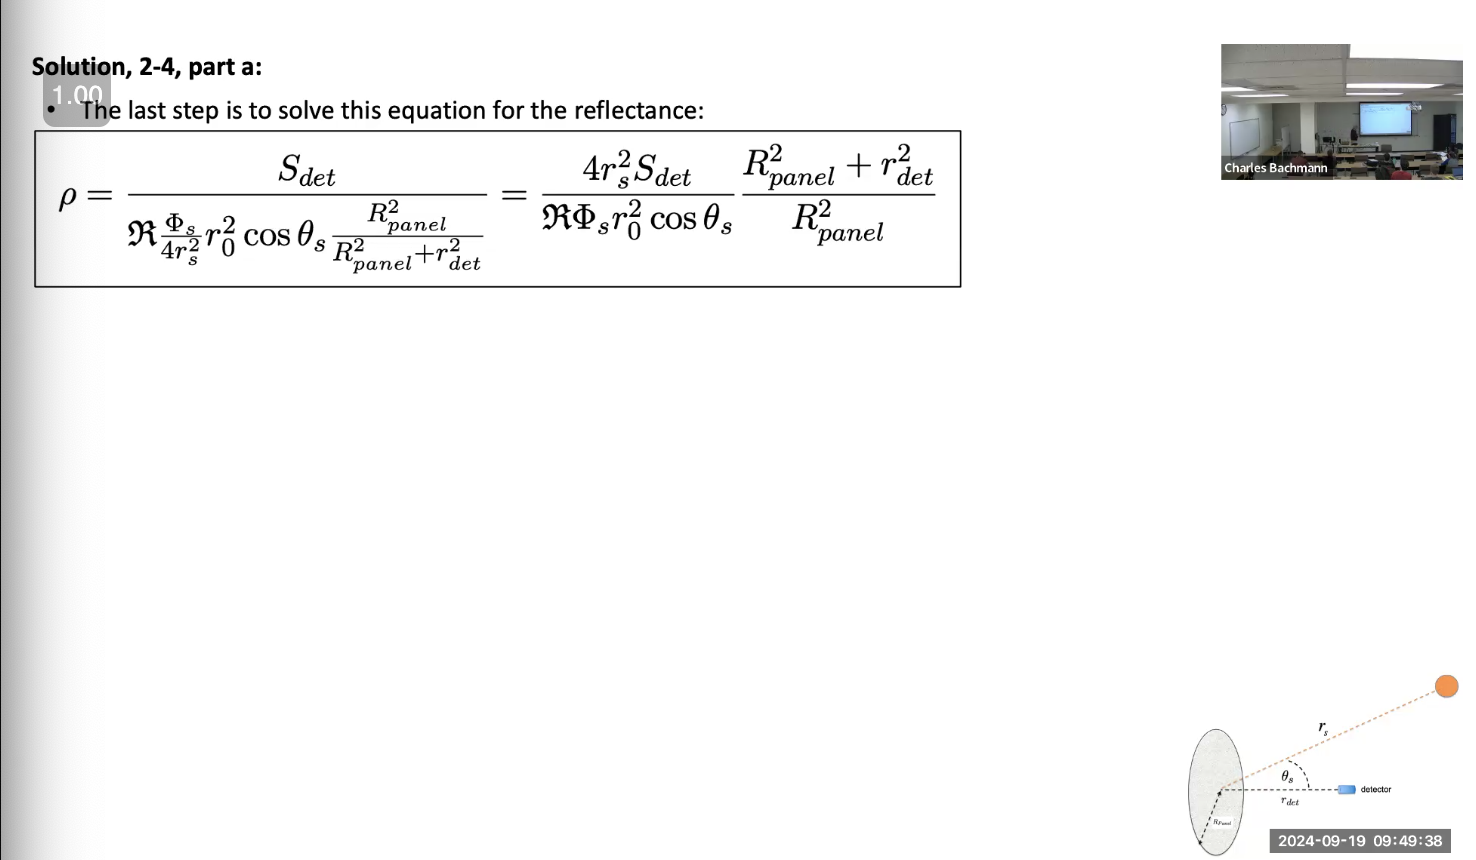
\includegraphics[scale=.6]{Radiometry/Week4/Notes/PSET2/P4/P4a.png}
\caption{Nugget the Snowman}
\label{fig:P4}
\end{figure}

\begin{figure}[h!]
\centering
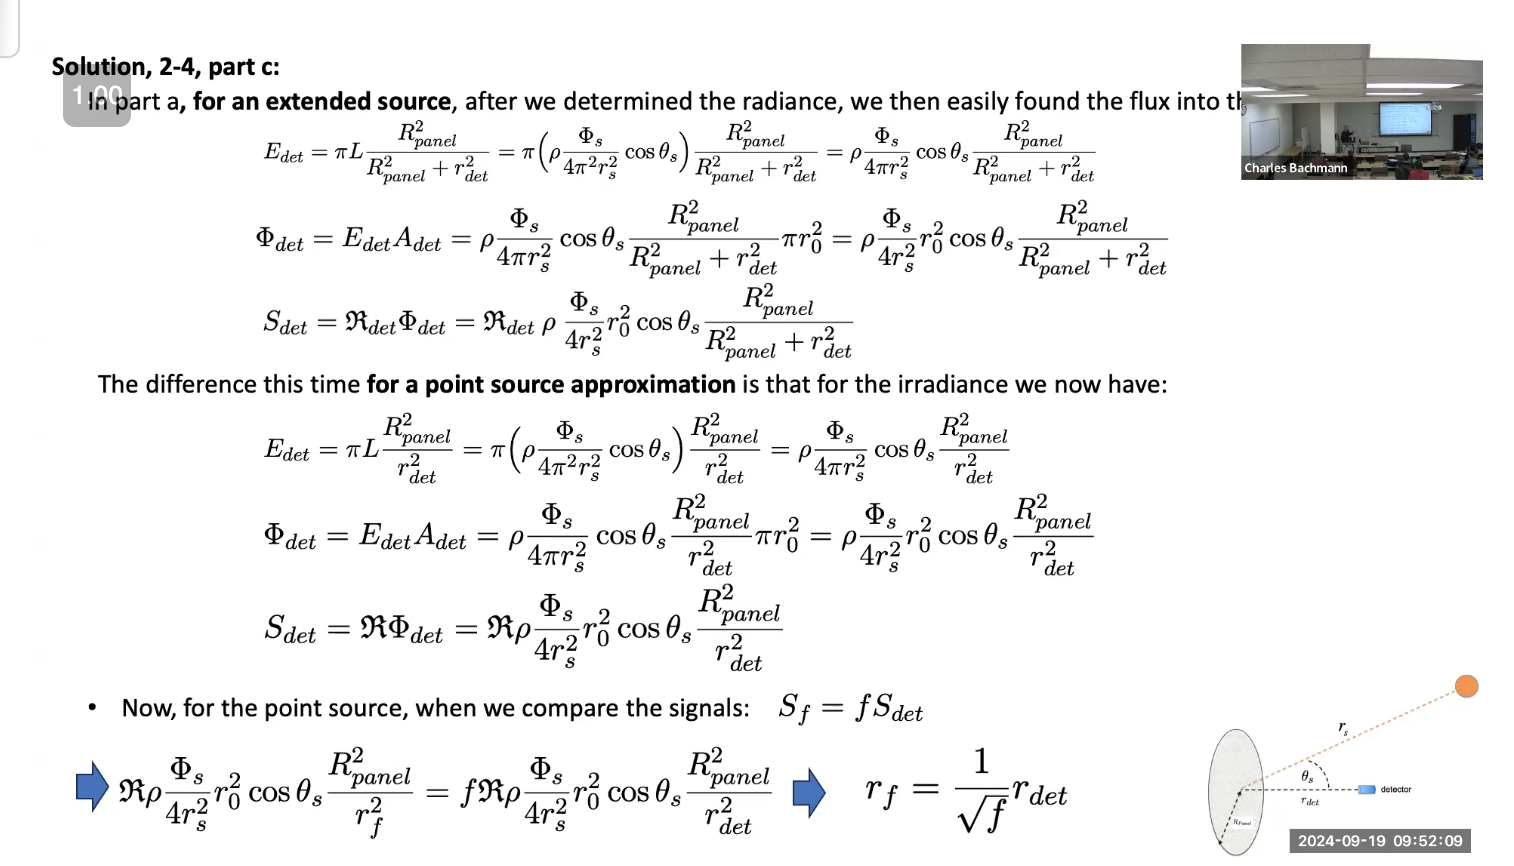
\includegraphics[scale=.6]{Radiometry/Week4/Notes/PSET2/P4/P4aa.png}
\caption{Nugget the Snowman}
\label{fig:P4}
\end{figure}


\clearpage
\subsubsection{Problem 5: Scattering and Greenstein and Rayleigh}
\begin{figure}[h!]
\centering
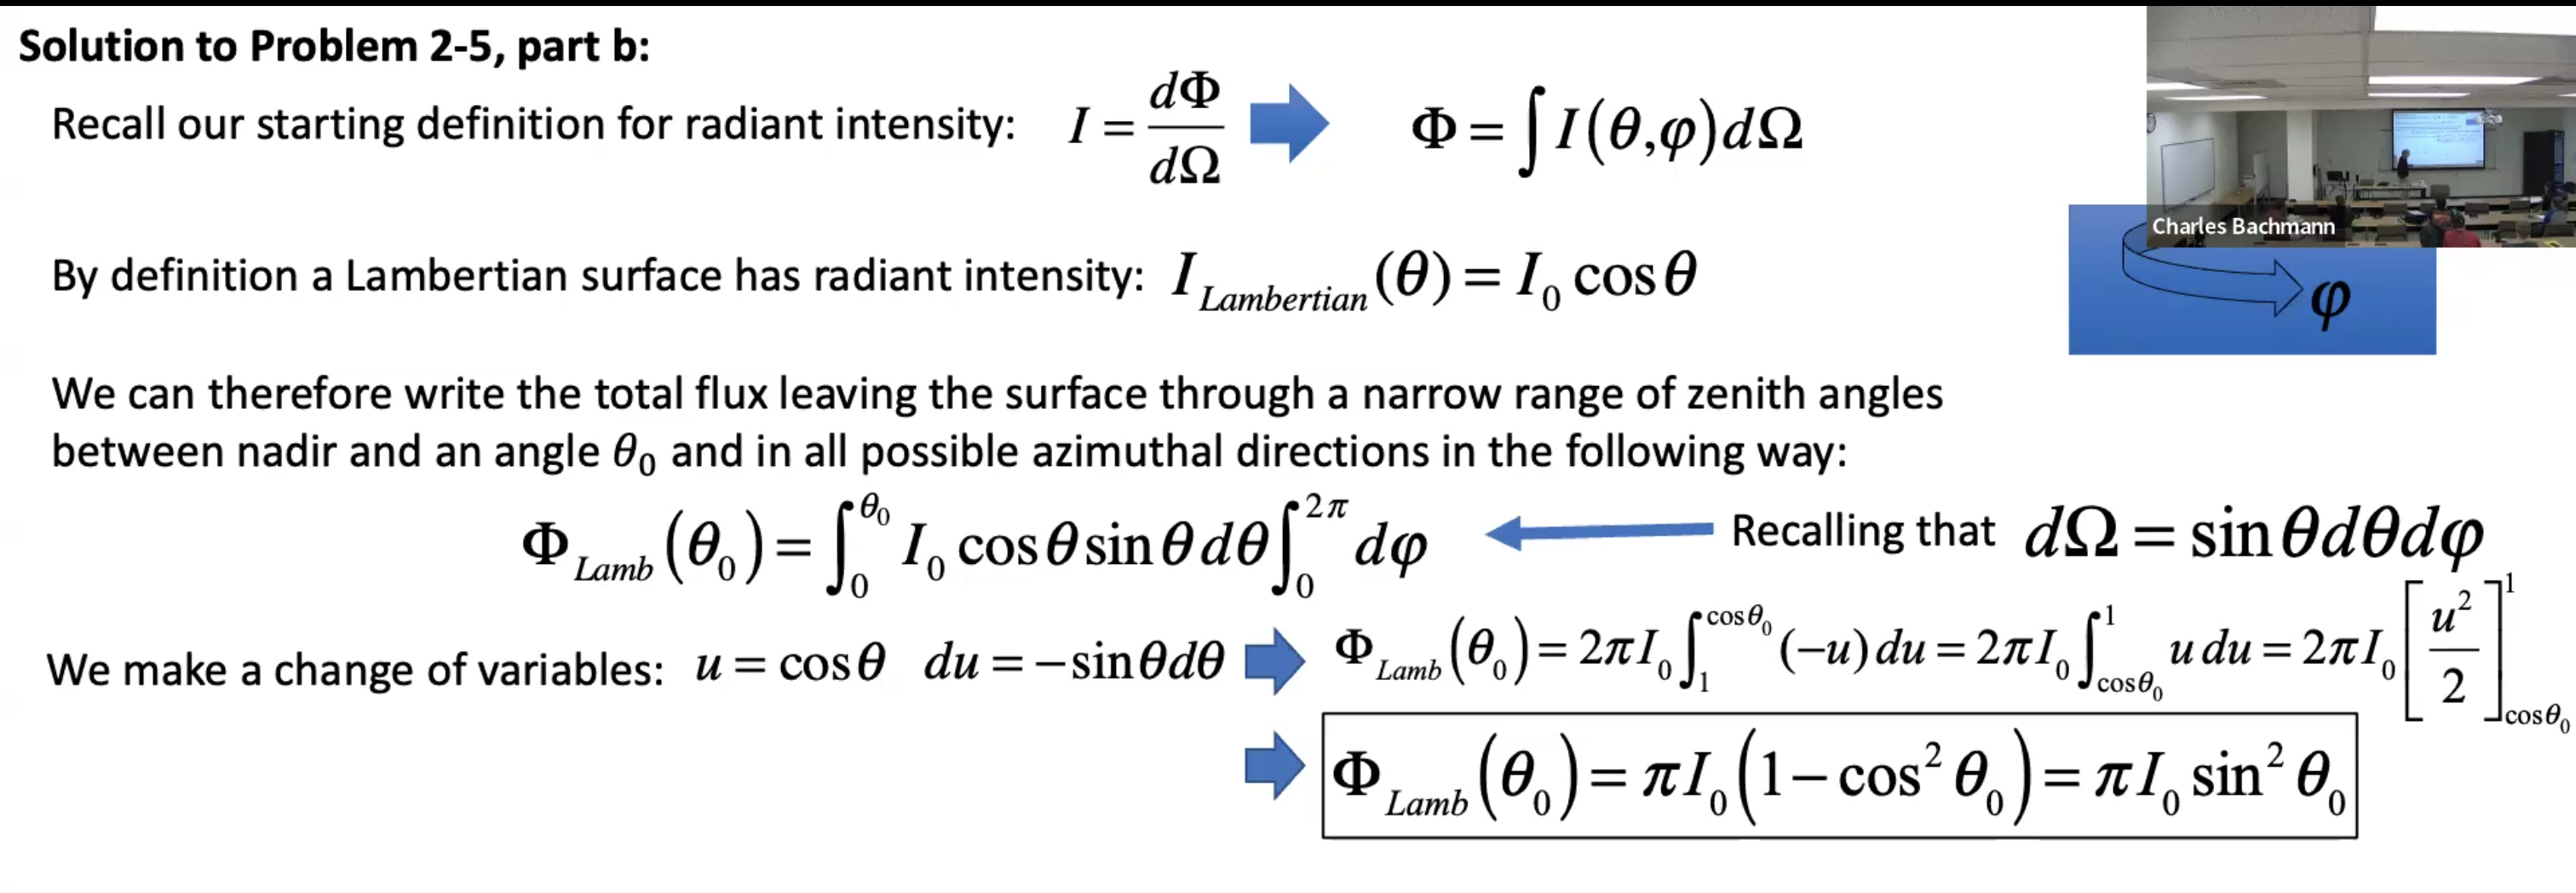
\includegraphics[scale=.2]{Radiometry/Week4/Notes/PSET2/P5/Num1.png}
\caption{Nugget the Snowman}
\label{fig:Greenstein}
\end{figure}

\begin{figure}[h!]
\centering
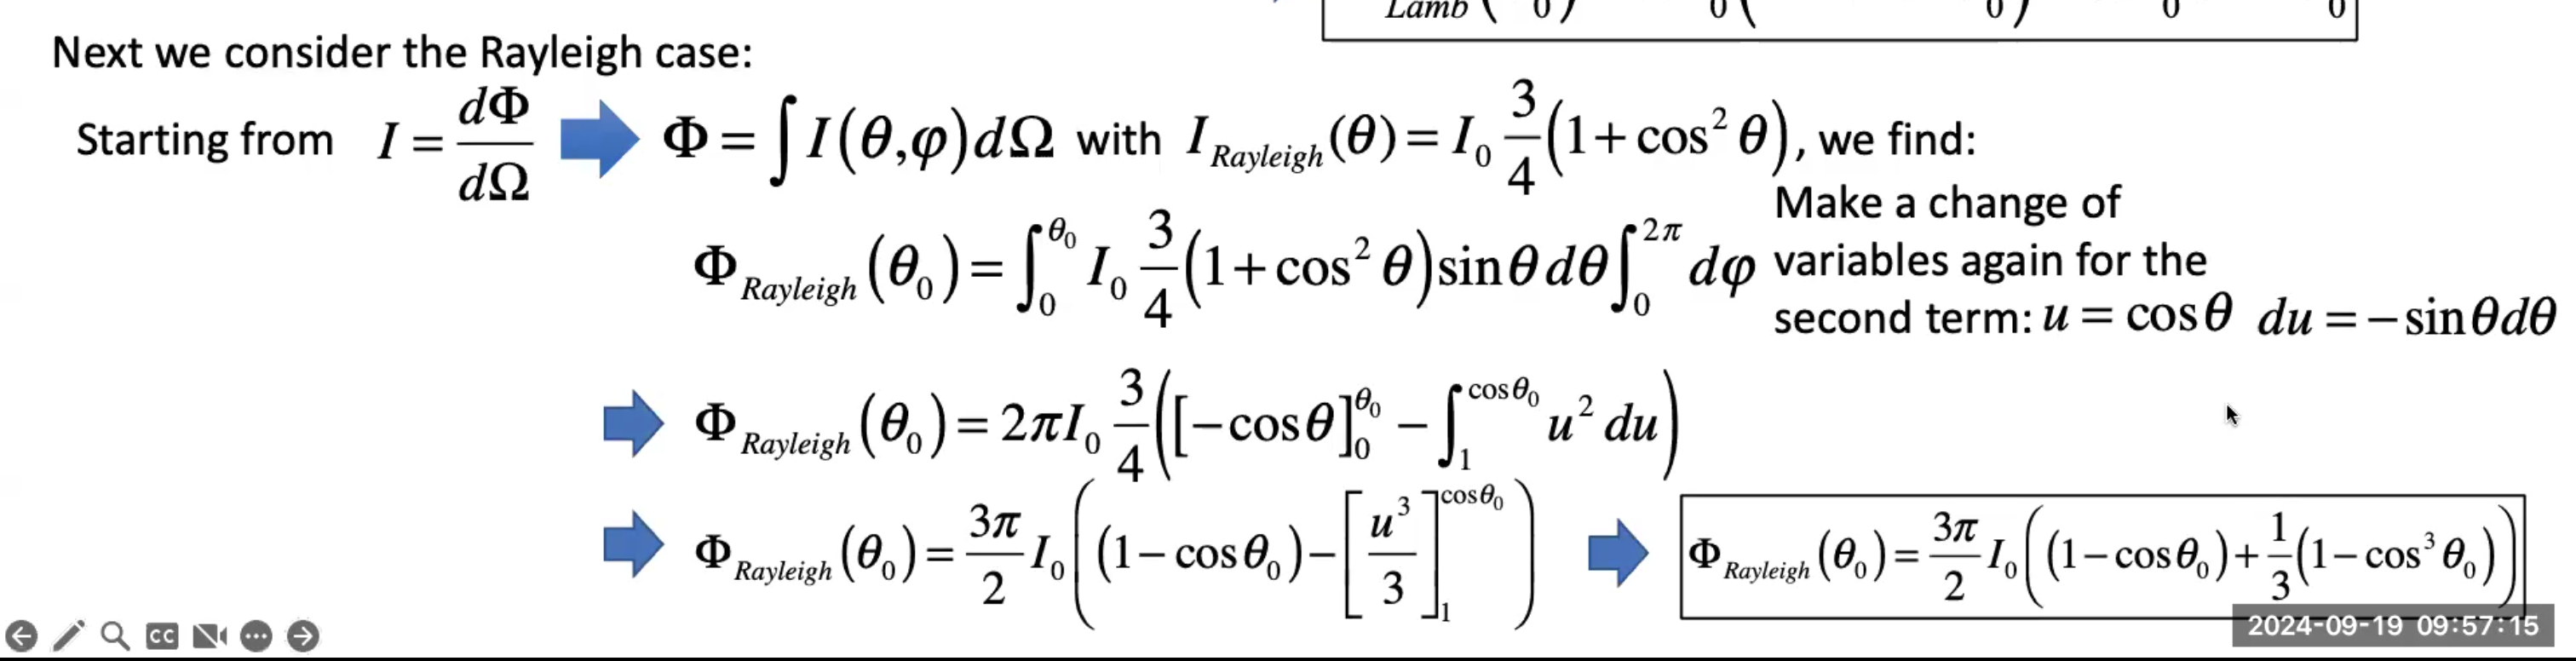
\includegraphics[scale=.2]{Radiometry/Week4/Notes/PSET2/P5/Num2.png}
\caption{Nugget the Snowman}
\label{fig:Greenstein}
\end{figure}

\begin{figure}[h!]
\centering
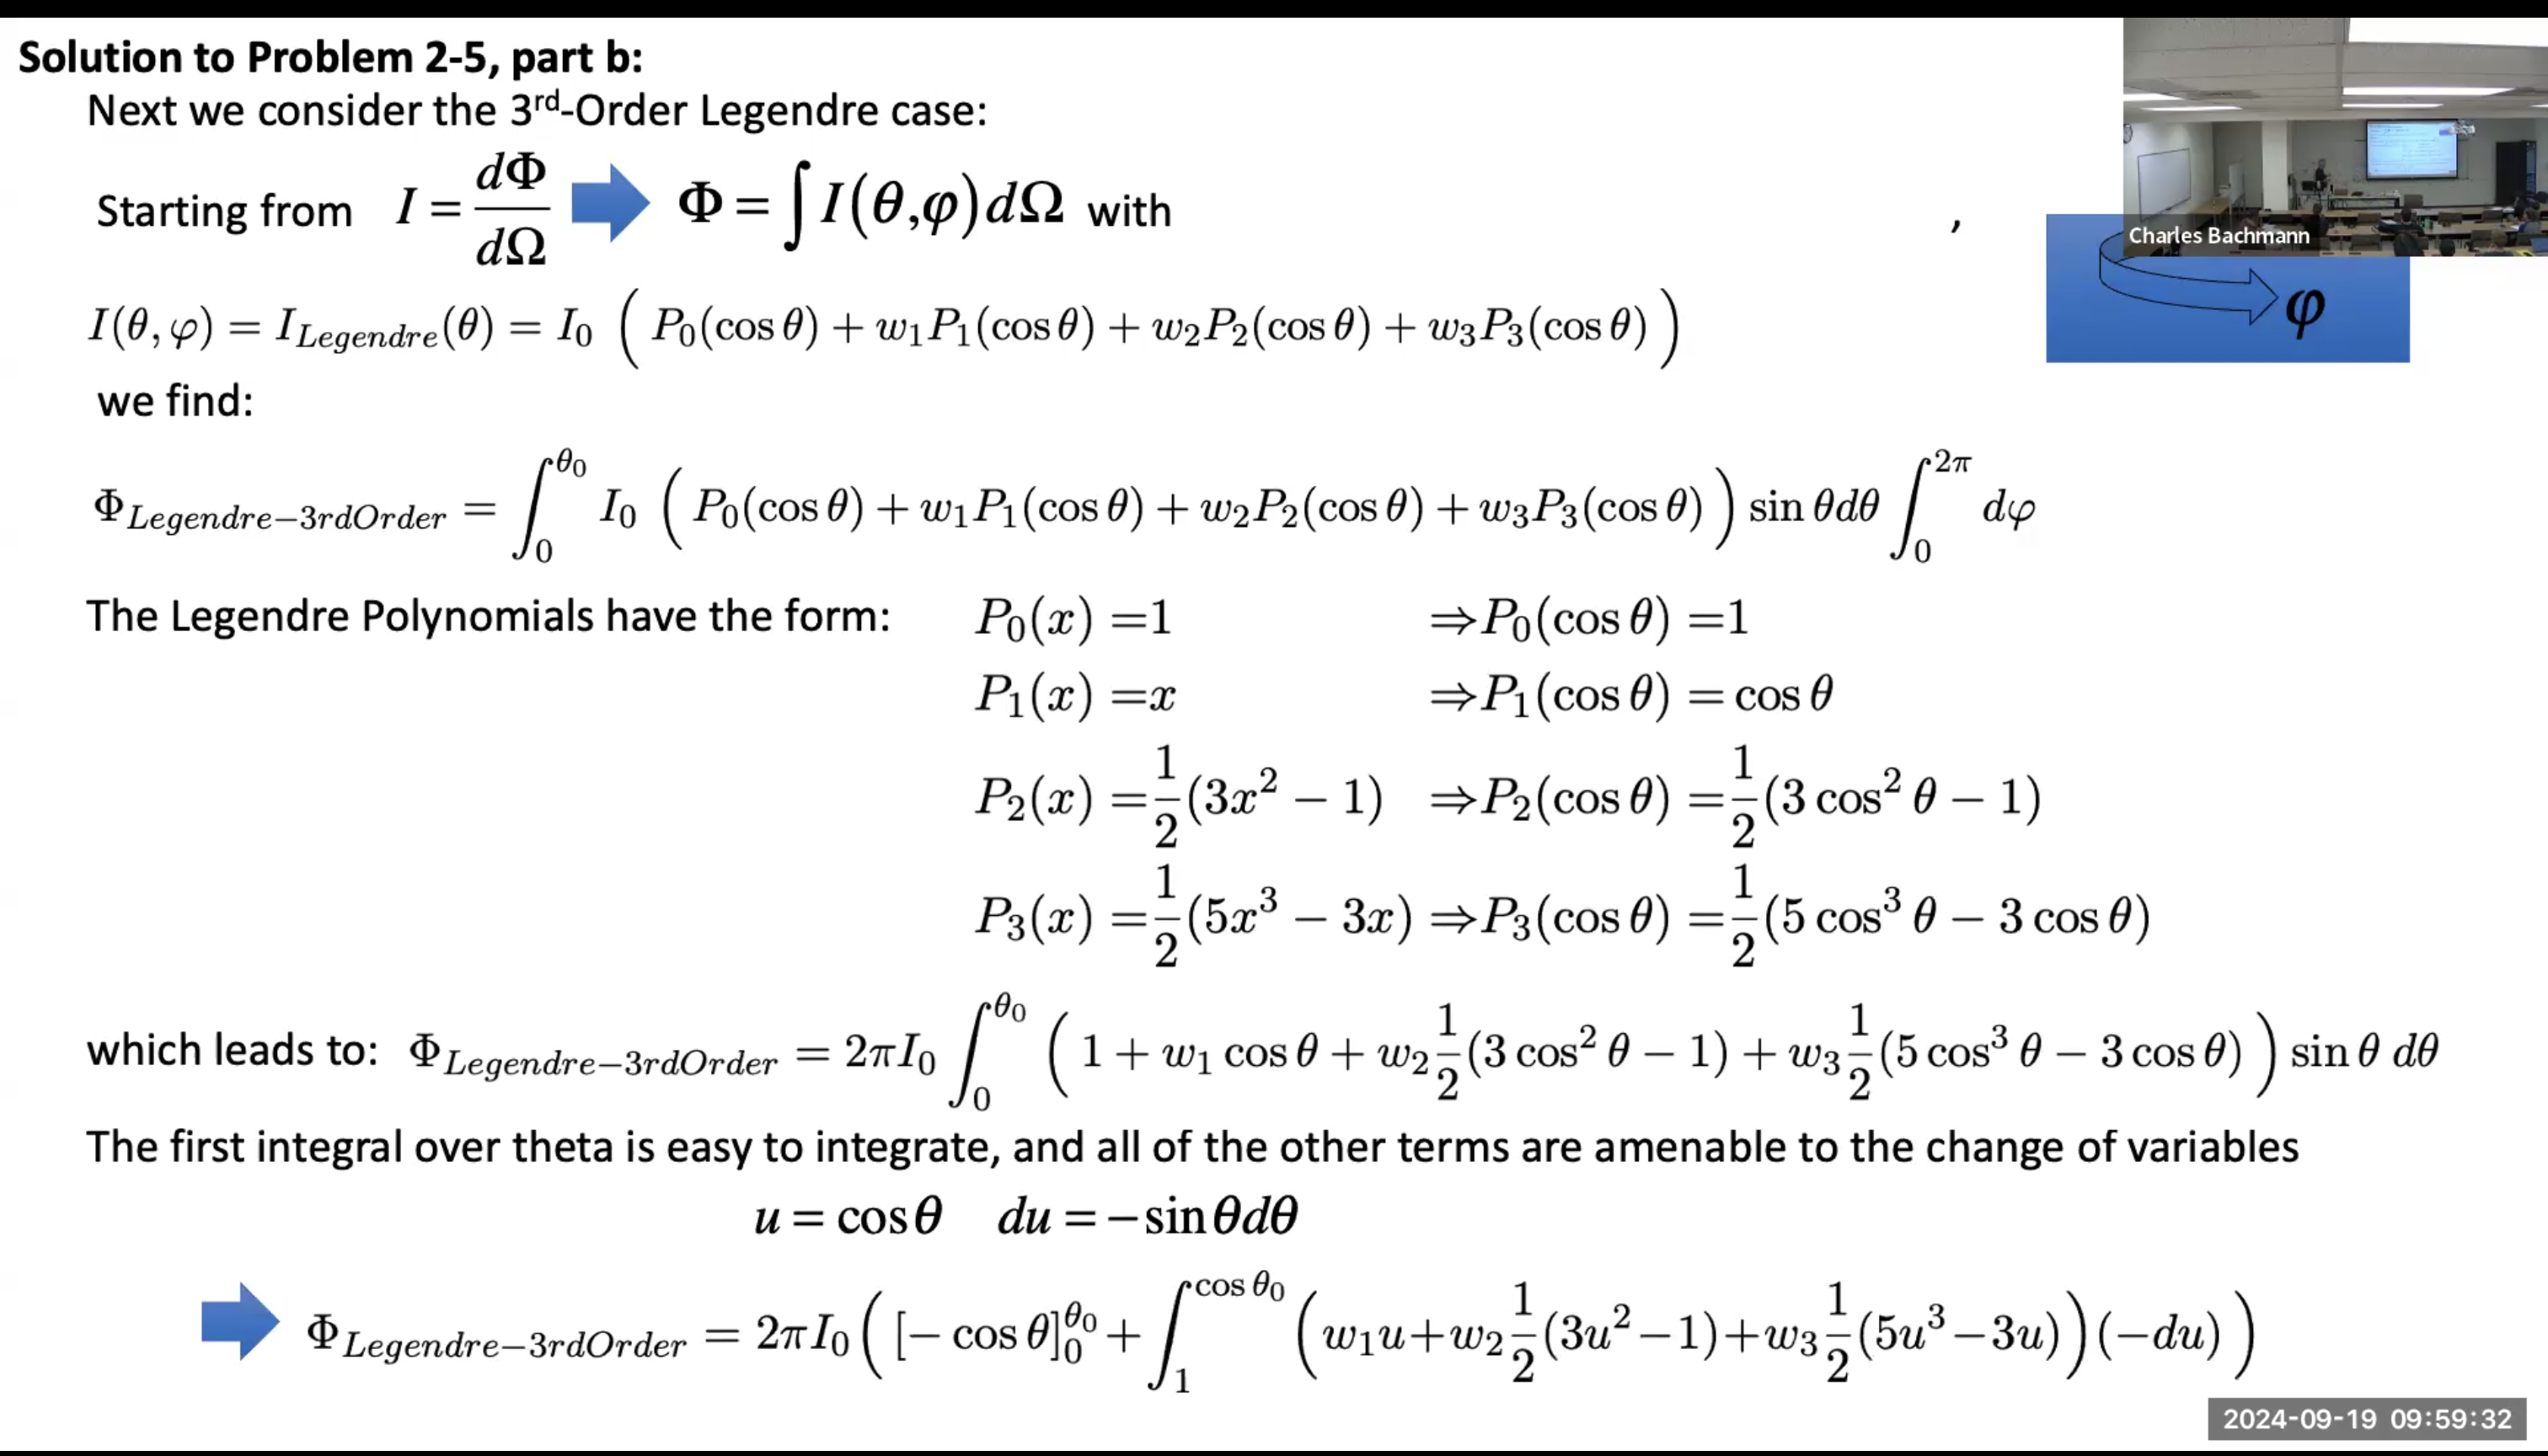
\includegraphics[scale=.2]{Radiometry/Week4/Notes/PSET2/P5/Num3.png}
\caption{Nugget the Snowman}
\label{fig:Greenstein}
\end{figure}

\begin{figure}[h!]
\centering
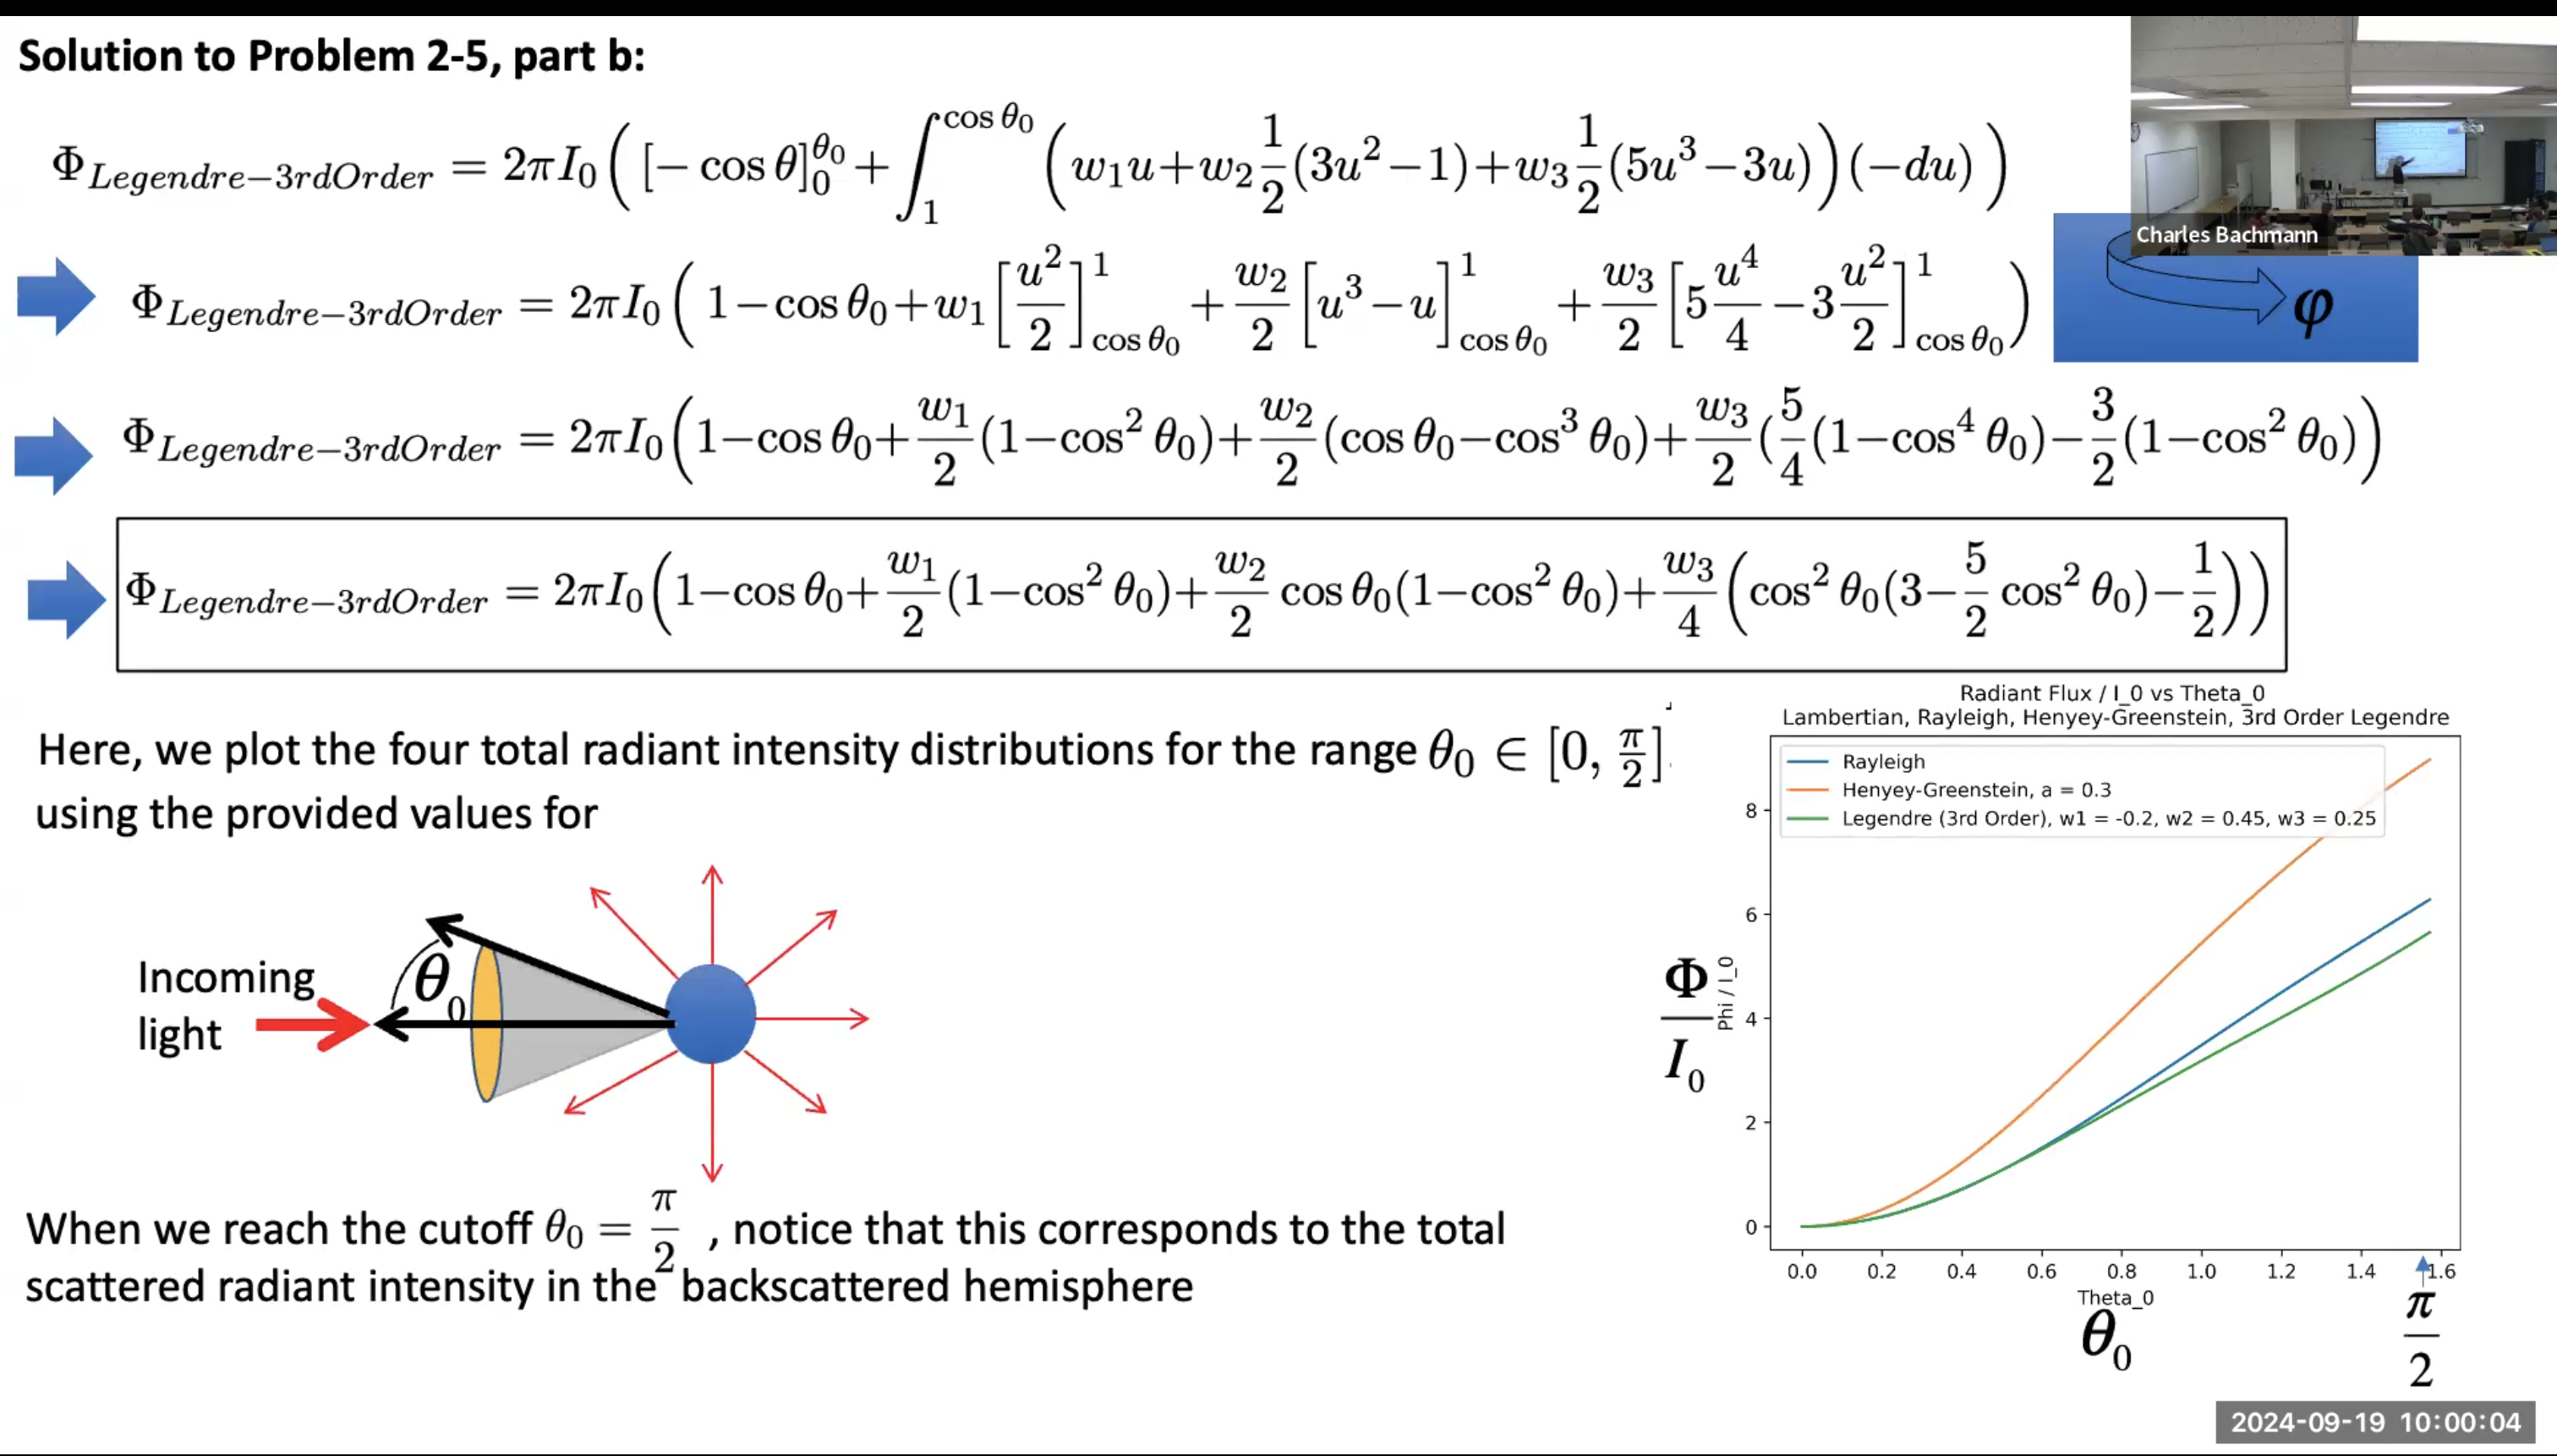
\includegraphics[scale=.2]{Radiometry/Week4/Notes/PSET2/P5/Num4.png}
\caption{Nugget the Snowman}
\label{fig:Greenstein}
\end{figure}
\begin{figure}[h!]
\centering
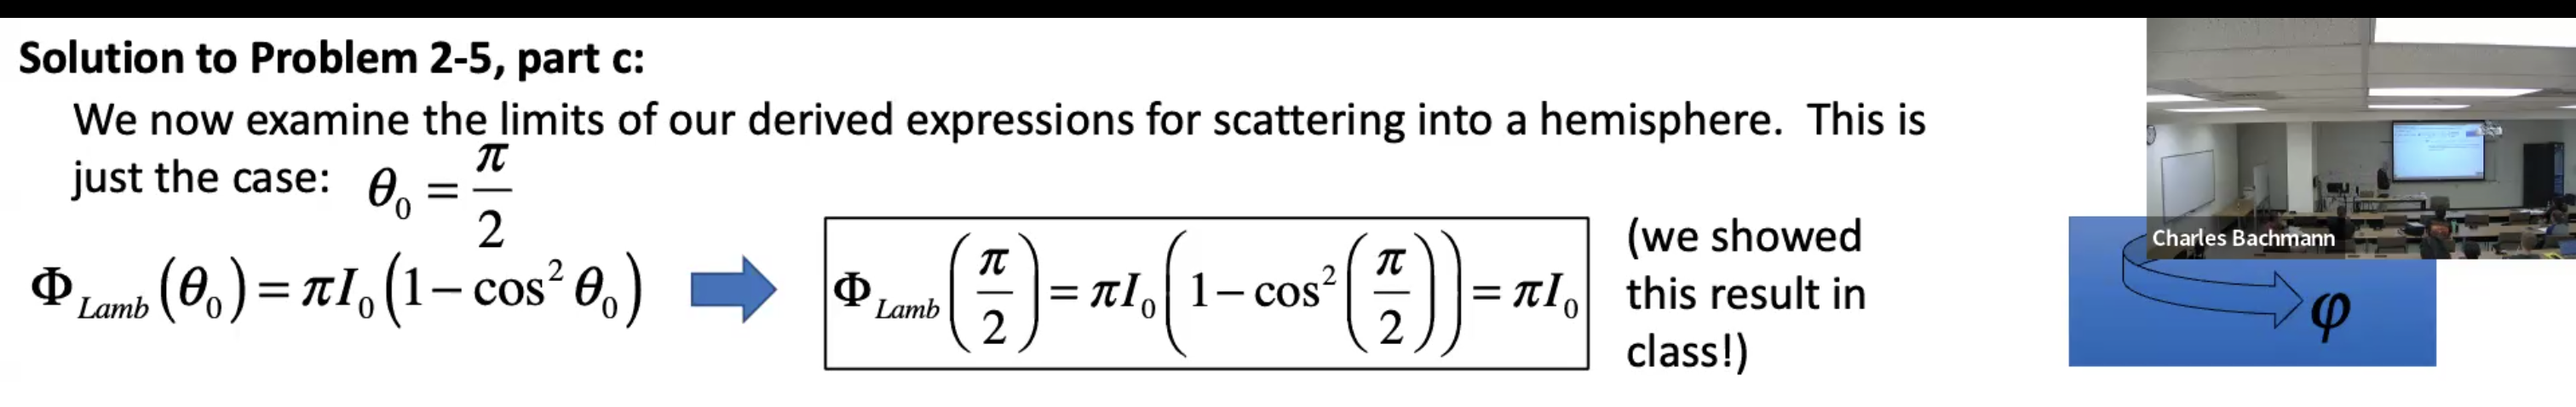
\includegraphics[scale=.2]{Radiometry/Week4/Notes/PSET2/P5/Num5.png}
\caption{Nugget the Snowman}
\label{fig:Greenstein}
\end{figure}


\begin{figure}[h!]
\centering
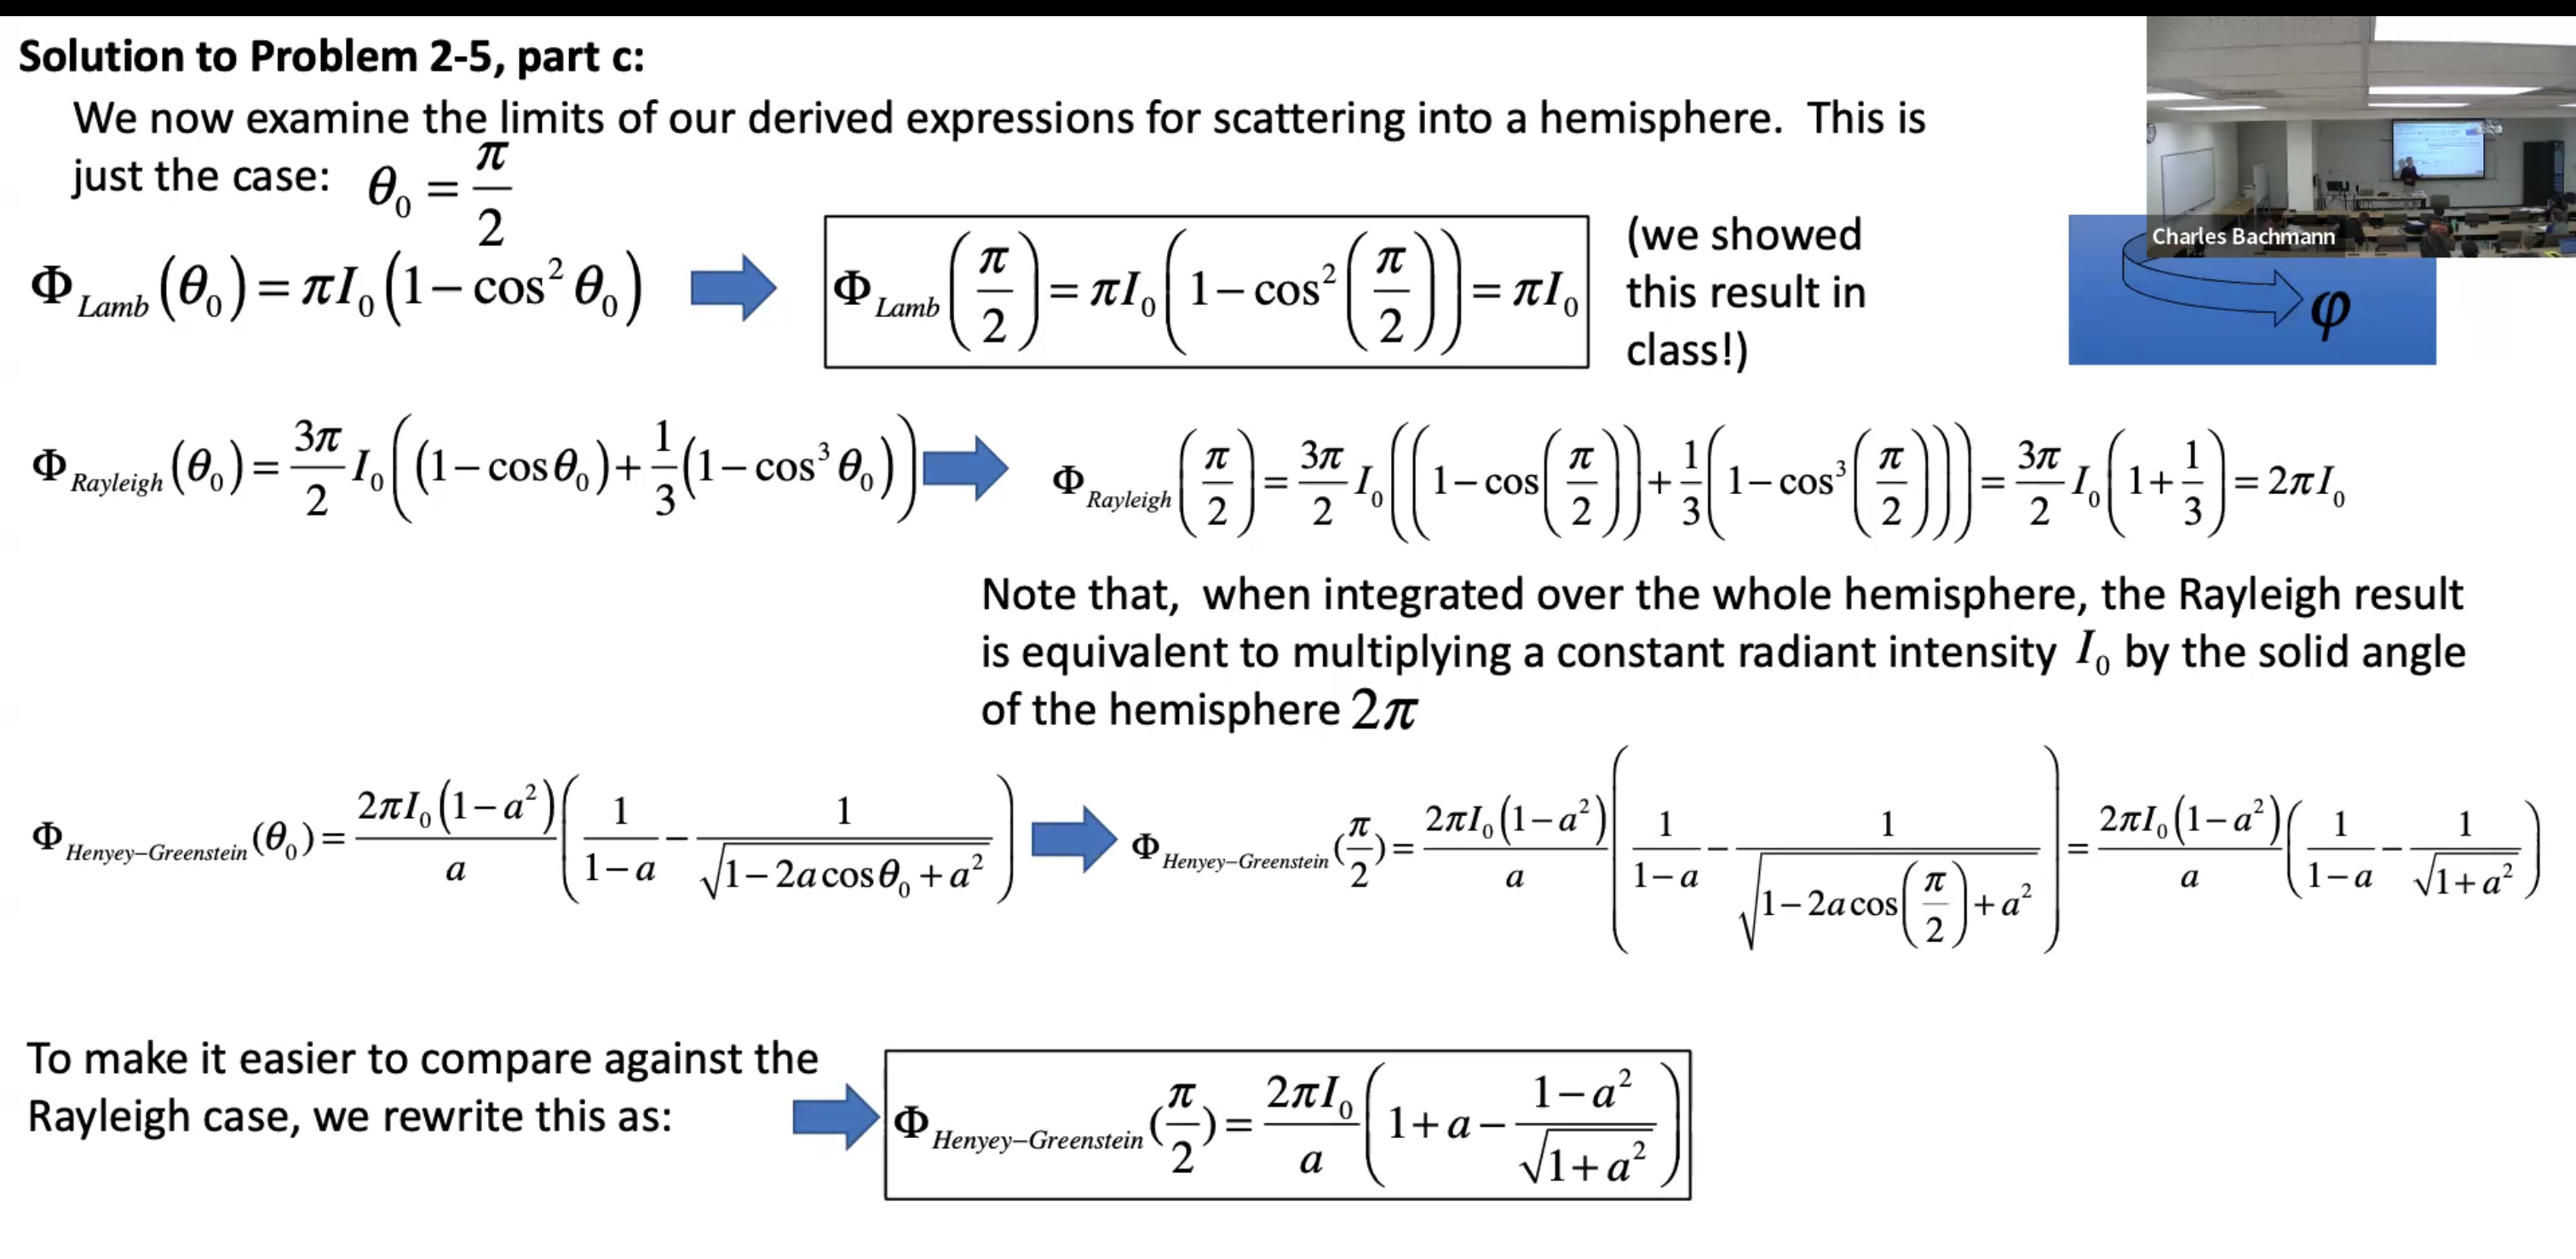
\includegraphics[scale=.2]{Radiometry/Week4/Notes/PSET2/P5/Num6.png}
\caption{Nugget the Snowman}
\label{fig:Greenstein}
\end{figure}

\begin{figure}[h!]
\centering
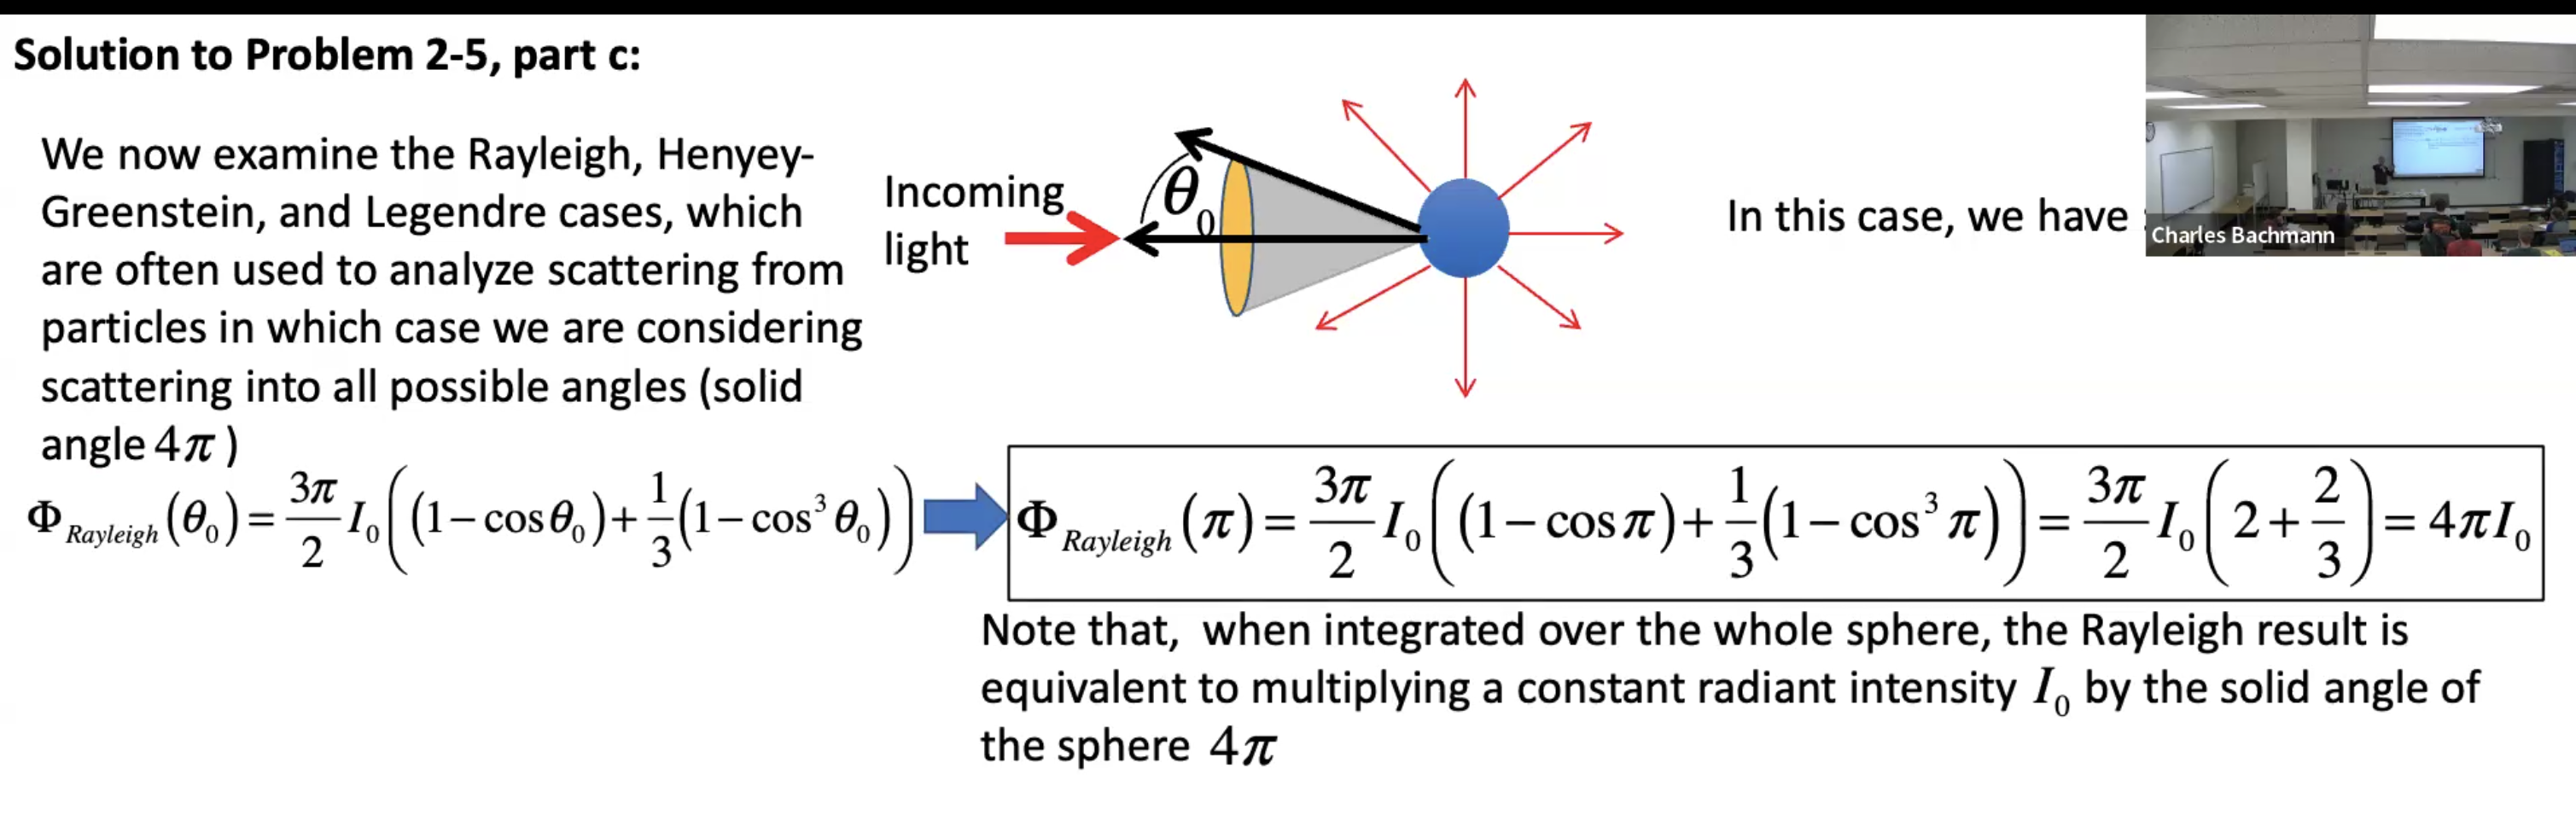
\includegraphics[scale=.2]{Radiometry/Week4/Notes/PSET2/P5/Num7.png}
\caption{Nugget the Snowman}
\label{fig:Greenstein}
\end{figure}



\begin{figure}[h!]
\centering
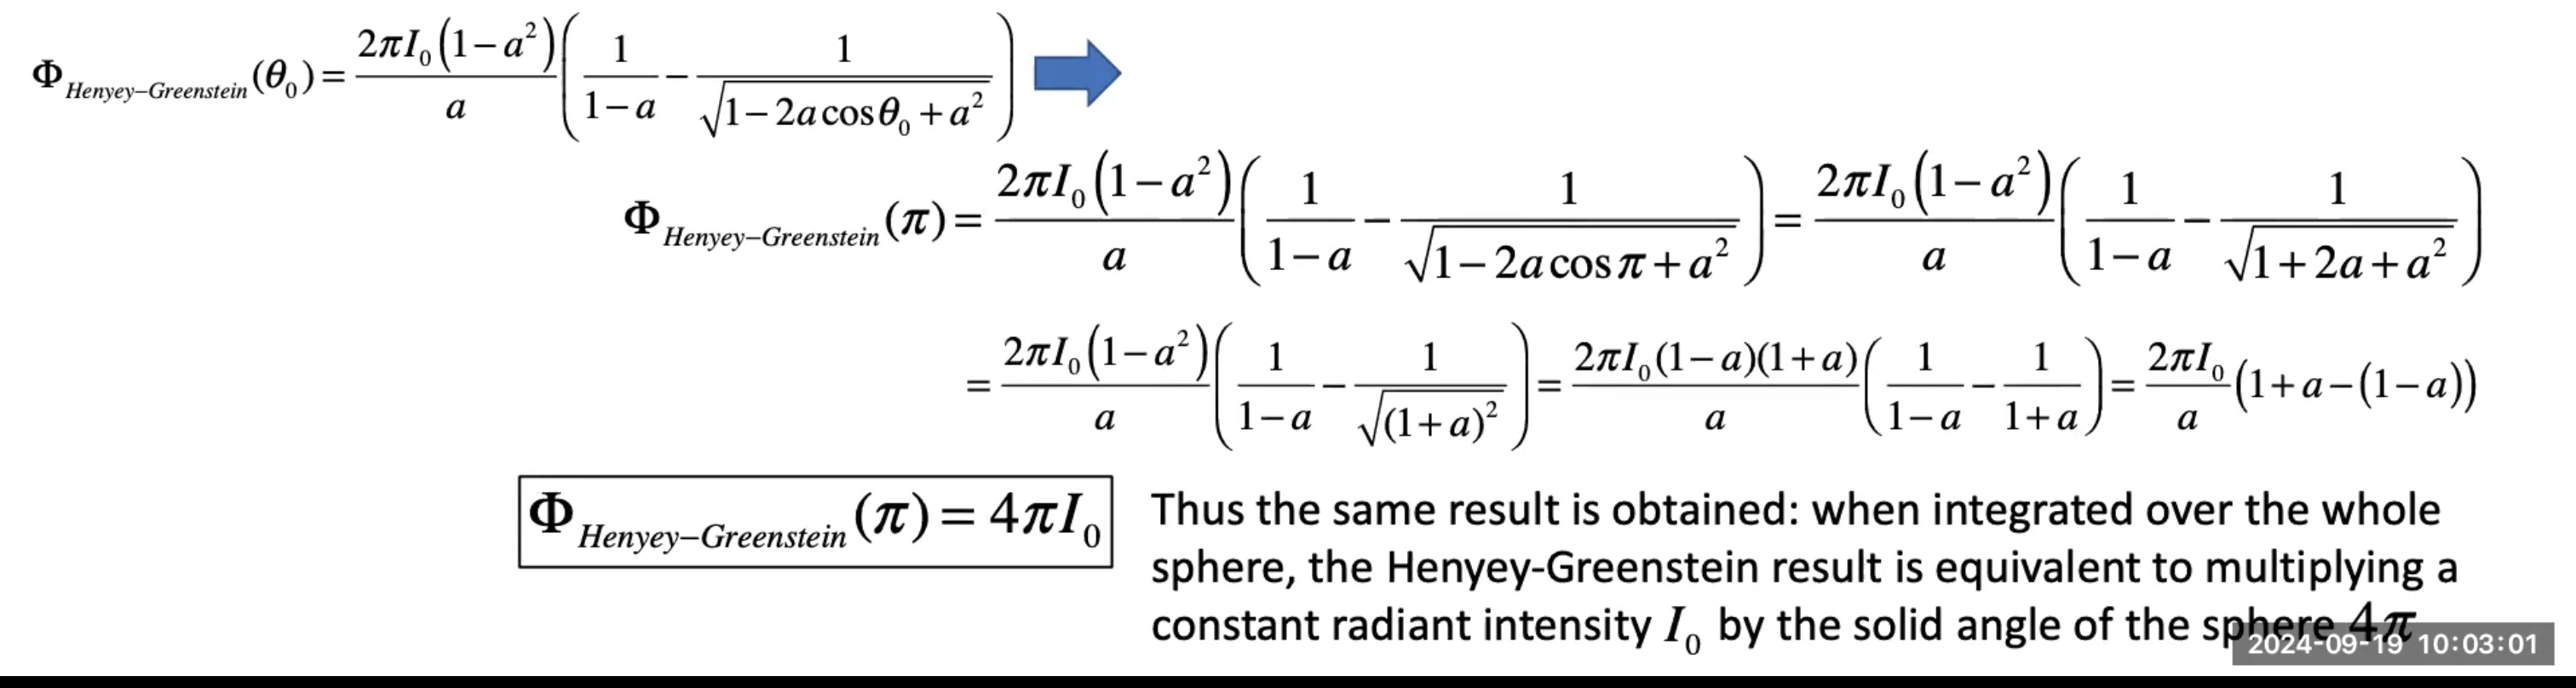
\includegraphics[scale=.2]{Radiometry/Week4/Notes/PSET2/P5/Num8.png}
\caption{Nugget the Snowman}
\label{fig:Greenstein}
\end{figure}


\begin{figure}[h!]
\centering
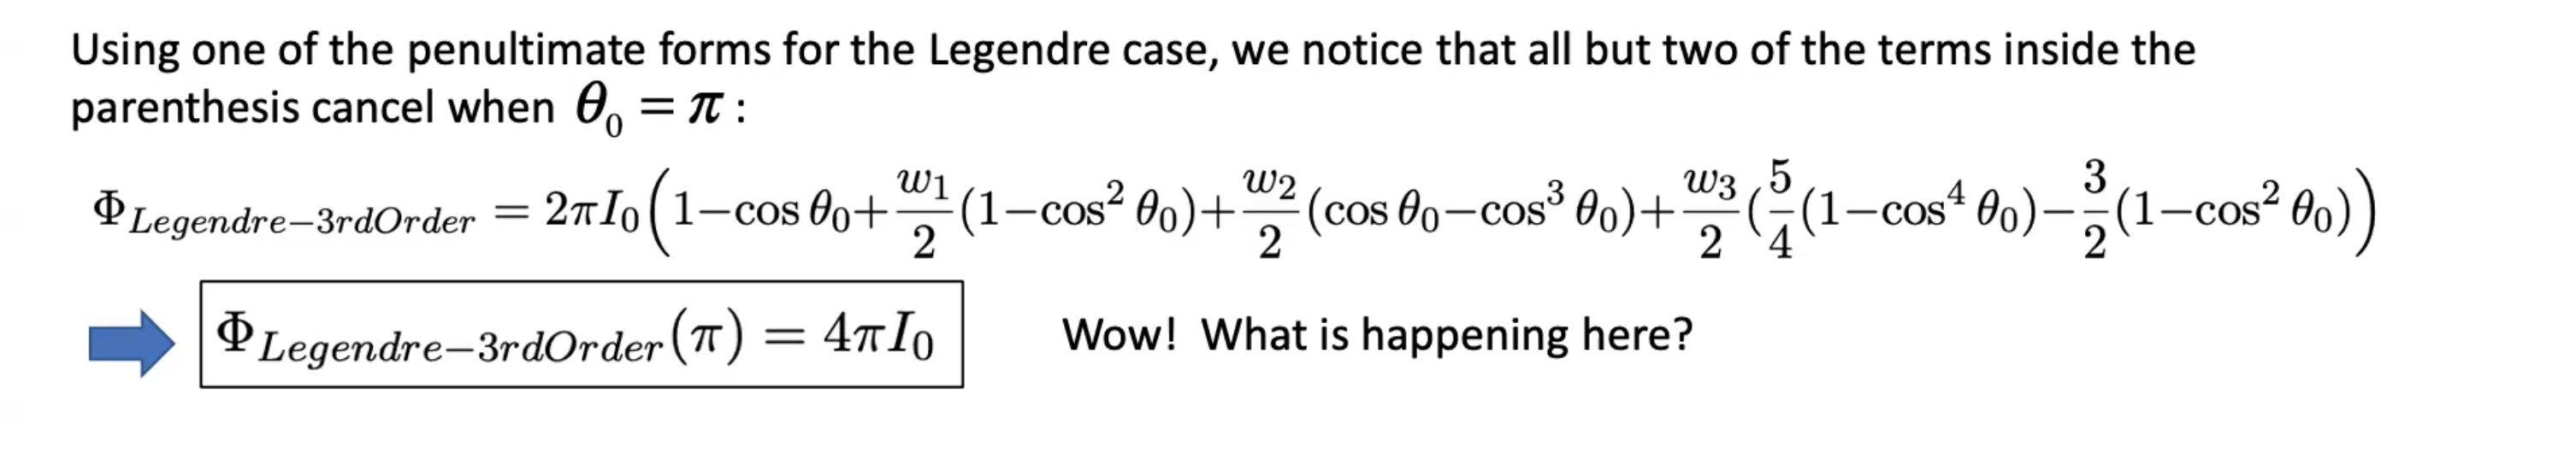
\includegraphics[scale=.2]{Radiometry/Week4/Notes/PSET2/P5/Num9.png}
\caption{Nugget the Snowman}
\label{fig:Greenstein}
\end{figure}


\begin{figure}[h!]
\centering
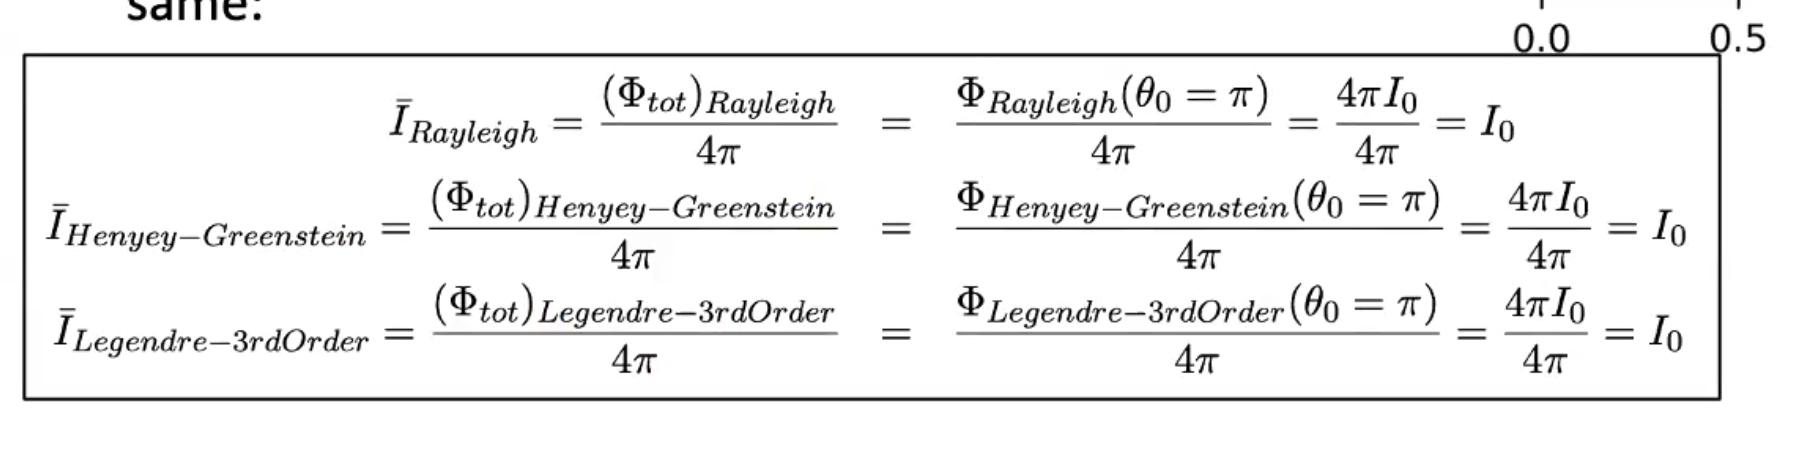
\includegraphics[scale=.2]{Radiometry/Week4/Notes/PSET2/P5/Num10.png}
\caption{Nugget the Snowman}
\label{fig:Greenstein}
\end{figure}
\clearpage

\subsection{ September 24th, 2024 : Week 5}

From last class 

\begin{figure}[h!]
\centering
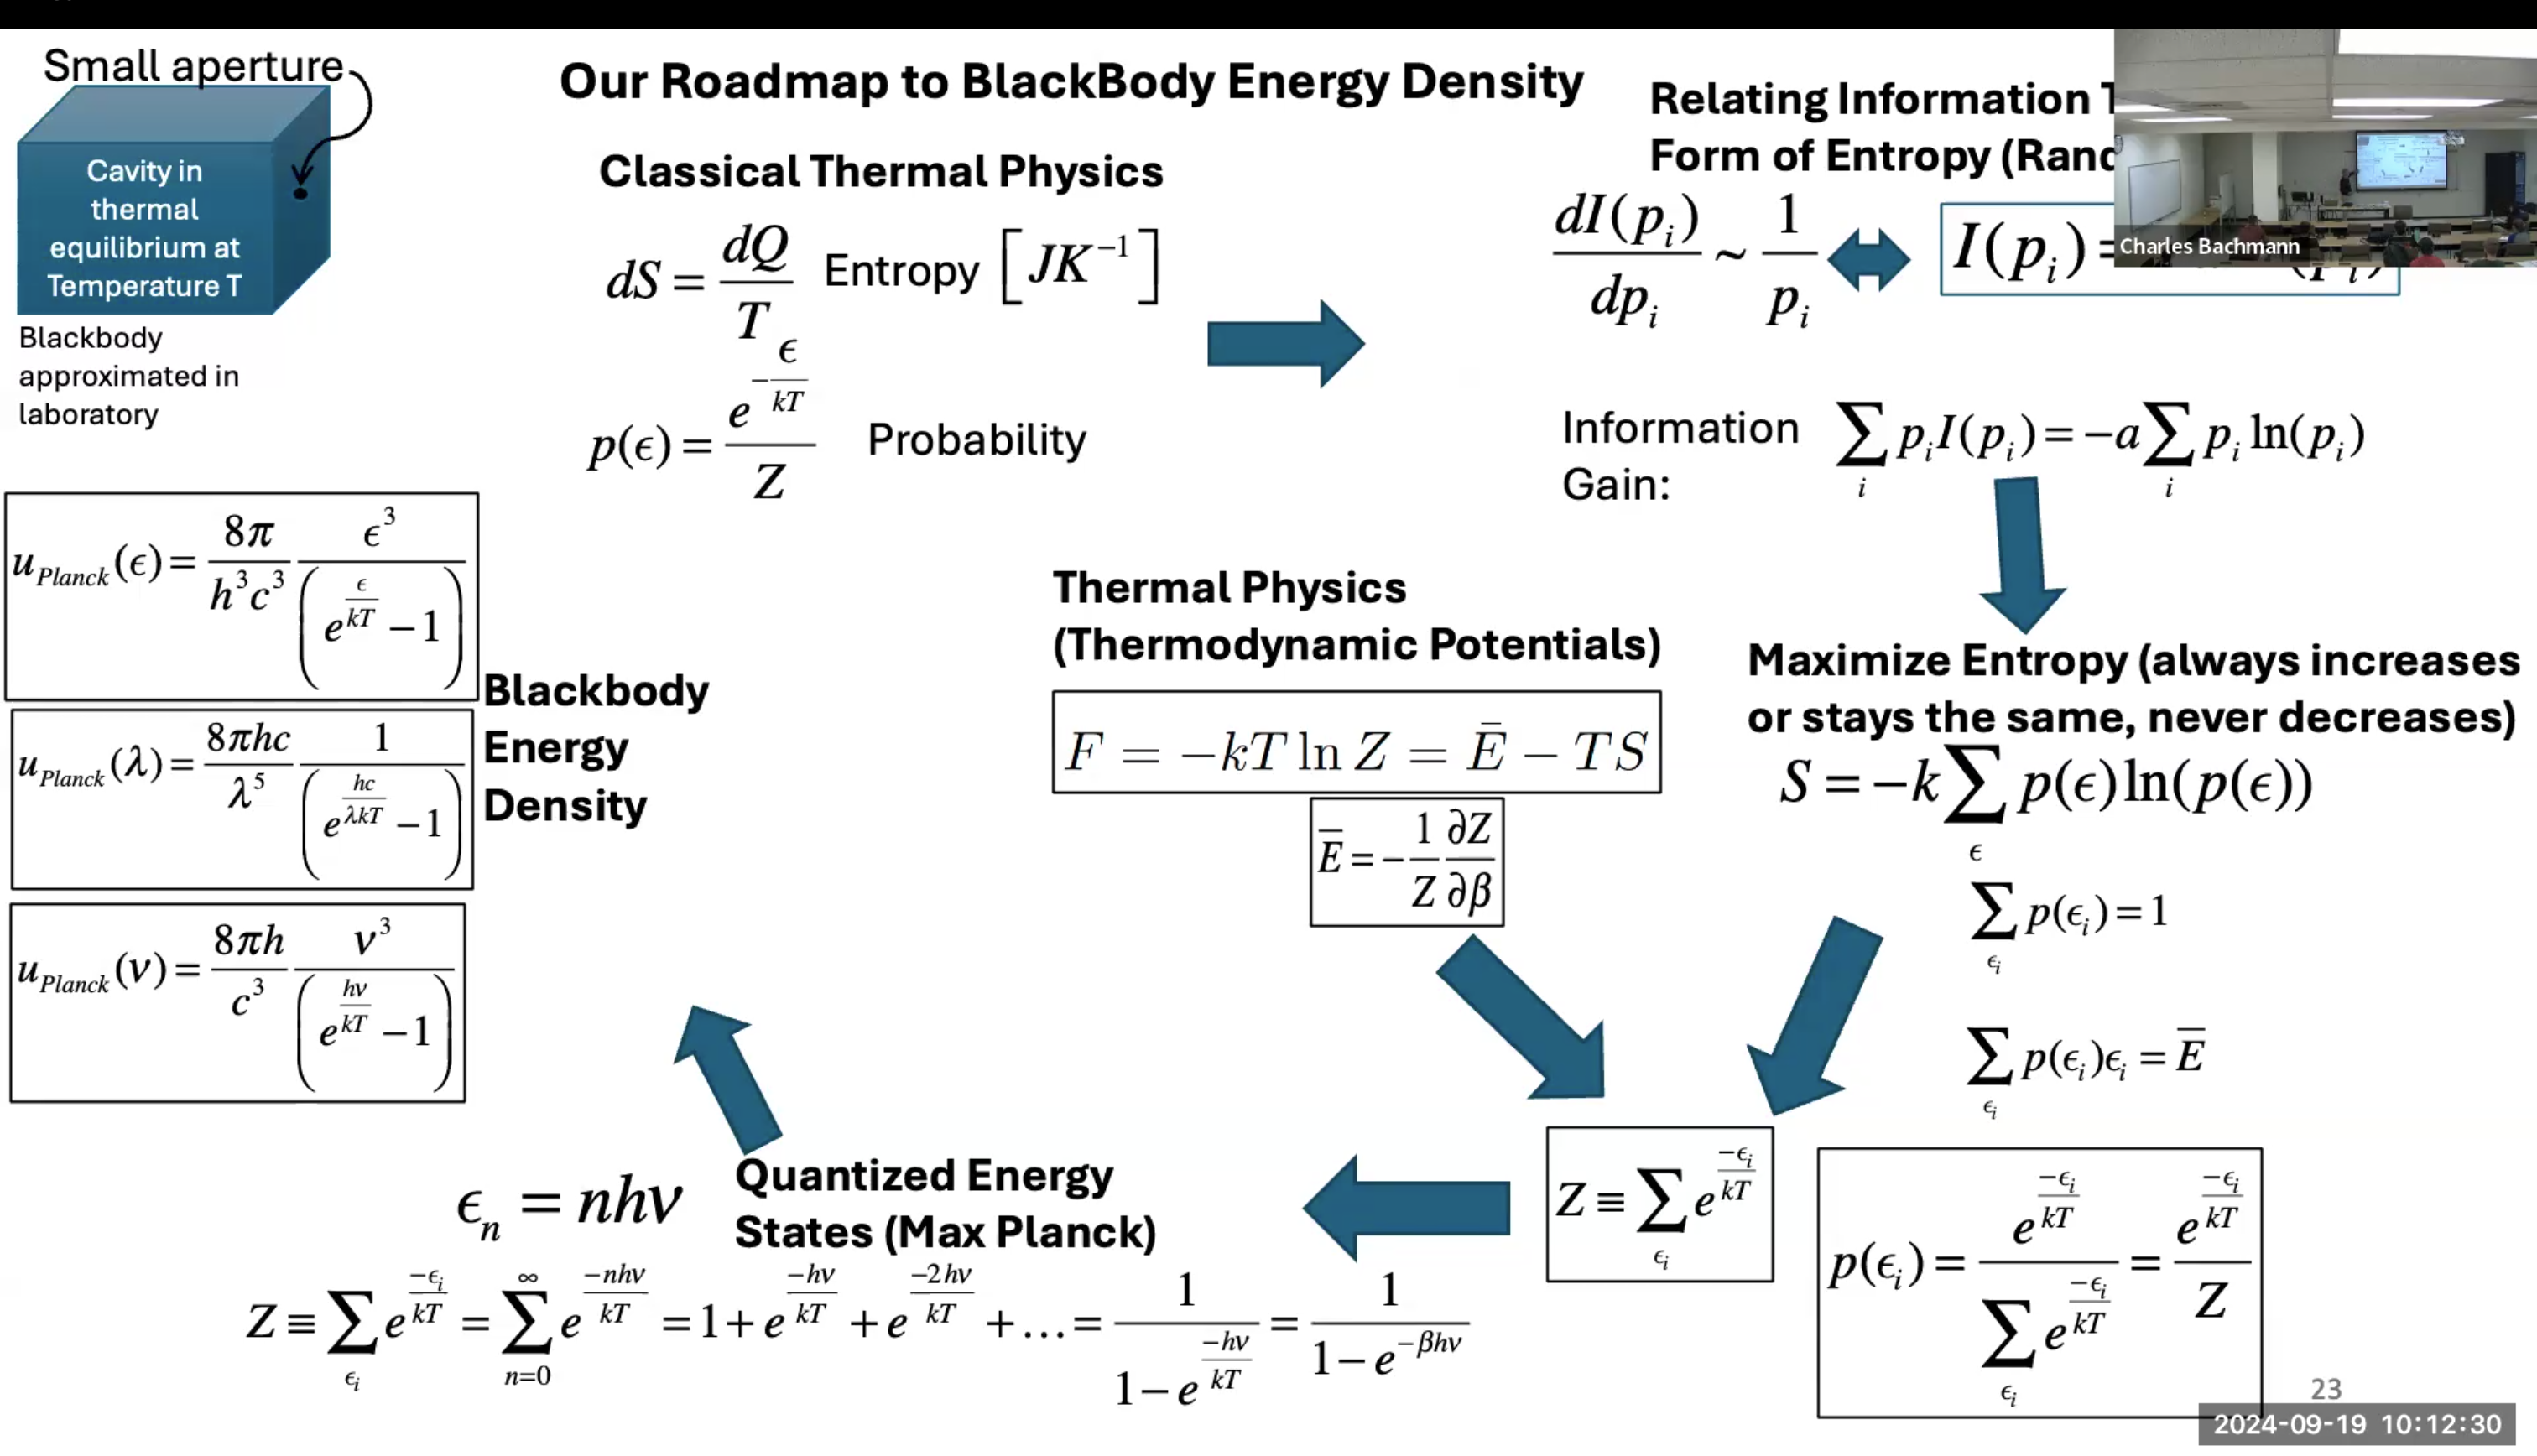
\includegraphics[scale=.3]{Radiometry/Week4/Notes/PSET2/BlackbodyIMP.png}
\caption{Nugget the Snowman}
\label{fig:Blackbody}
\end{figure}


\begin{figure}[h!]
\centering
\includegraphics[scale=.6]{Radiometry/Week4/Notes/PSET2/Gradiant.png}
\caption{Nugget the Snowman}
\label{fig:Blackbody}
\end{figure}
\clearpage
\subsection{September 26th, 2024 Week 5}
\begin{figure}[h!]
\centering
\includegraphics[scale=.4]{Radiometry/Week5/Notes/Gratings/MUM1.png}
\caption{Gratings}
\label{fig:Blackbody}
\end{figure}

\begin{figure}[h!]
\centering
\includegraphics[scale=.4]{Radiometry/Week5/Notes/Gratings/MUM2.png}
\caption{Gratings}
\label{fig:Blackbody}
\end{figure}


\begin{figure}[h!]
\centering
\includegraphics[scale=.4]{Radiometry/Week5/Notes/Gratings/MUM3.png}
\caption{Gratings}
\label{fig:Blackbody}
\end{figure}

\begin{figure}[h!]
\centering
\includegraphics[scale=.4]{Radiometry/Week5/Notes/Gratings/MUM4.png}
\caption{Gratings}
\label{fig:Blackbody}
\end{figure}

\begin{figure}[h!]
\centering
\includegraphics[scale=.4]{Radiometry/Week5/Notes/Gratings/MUM5.png}
\caption{Gratings}
\label{fig:Blackbody}
\end{figure}

\begin{figure}[h!]
\centering
\includegraphics[scale=.4]{Radiometry/Week5/Notes/Gratings/MUM6.png}
\caption{Gratings}
\label{fig:Blackbody}
\end{figure}

\begin{figure}[h!]
\centering
\includegraphics[scale=.4]{Radiometry/Week5/Notes/Gratings/MUM1.png}
\caption{Gratings}
\label{fig:Blackbody}
\end{figure}

\begin{figure}[h!]
\centering
\includegraphics[scale=.4]{Radiometry/Week5/Notes/Gratings/MUM7.png}
\caption{Gratings}
\label{fig:Blackbody}
\end{figure}

\begin{figure}[h!]
\centering
\includegraphics[scale=.4]{Radiometry/Week5/Notes/Gratings/MUM8.png}
\caption{Gratings}
\label{fig:Blackbody}
\end{figure}

\begin{figure}[h!]
\centering
\includegraphics[scale=.4]{Radiometry/Week5/Notes/Gratings/MUM9.png}
\caption{Gratings}
\label{fig:Blackbody}
\end{figure}


\subsection{October 1st, 2024: Week 6 GRATINGS}



\clearpage


\subsection{October 3rd, 2024}






\clearpage
\section{Key Terms, and Things to Remember (Mid-term)} 
\begin{itemize}
\item Non-Point Sources
\item Black body diagrams
\item Radiance
\item No derivations of blackbodies
\item Parameterization of stuff and that NASA problem 7 on pset 2
\item Solid Angle 
\item HW 2.2. Problem seems like a good problem
\item All the different definitions around radiance, irradiance, radiant intensity etc.
\item Review integration by parts and u substitution 
  %\begin{itemize}
    %\item This is an even function
    %\item He loves it being piecewise as well.
  %\end{itemize}

% \begin{figure}[h!]
% \centering
% \includegraphics[scale=.20]{Fourier/unnamed.jpg}
% \caption{Easton Syllabus}
% \label{fig:Snowman4}
% \end{figure}


 
\end{itemize}

\clearpage


% \[
%     V= \frac{4}{3} \pi (b^3 + c^3 + f^3)    
% \]


% \[
%     V= \frac{4}{3} \pi (2^3 + 1.75^3 + 1^3)    
% \]

% \[
%     V= \frac{4}{3} \pi (8 + 5.359375 + 1)    
% \]

% \[
%     V= \frac{4}{3} \pi (8 + 5.359375 + 1)    
% \]

% \[
%     V= 19.1458333 \pi \; ft^3  
% \]



% \section{Question 3}        


% From before, 
% \[
%     V= \frac{4}{3} \pi (r^3)  
% \]

% Let C (t)= Volume of the center sphere at time t. 

% At t= 8 min. 


% \[
%     C = \frac{4}{3} \pi ((.75+.25(t-7))^3)  
% \]

% \[
%     \frac{dC}{dt}= \frac{4}{3} \pi ((.75+ \frac{8-7}{4})^2)\frac{dt}{dt} * (\frac{3}{4}) 
% \]
% \[
%     \frac{dC}{dt}= \pi ((.75+ \frac{t}{4})^2)
% \]

% \[
%     \frac{dC}{dt}= 4\pi (r(t))^2 * r'(t)
% \]

% \[
%     \frac{dC}{dt}= 4\pi (1)^2 * \frac{1}{4}
% \]

% \[
%     \frac{dC}{dt}= \pi \; \; \frac{ft^3}{min}
% \]
\subsection{Trig Identities}
\begin{equation}
    cos(\theta)= \frac{e^{i \theta}+e^{-i \theta}}{2}
\end{equation}

\begin{equation}
    sin(\theta)= \frac{e^{i \theta}-e^{-i \theta}}{2i}
\end{equation}
Don't forget to remember your adding exponents when their bases are being multiplied by each other!
\begin{equation}
    sin(\theta)= cos(\theta - \frac{\pi}{2}) 
\end{equation}
Never forget good old SOH CAH TOA. 
He has thrown in a nice small angle approximation before as well. 

\begin{figure}[h!]
\centering
\includegraphics[scale=.95]{Radiometry/Week1/Notes/Syllabus.png}
\caption{Course Syllabus: He goes through this pretty thoroughly, except that we did not get to Week 6. The exam is on 2,3,4,5, and 6.}
\label{fig:Snowman3}
\end{figure}



\section{Class Summary}


\subsection{Beginning to middle of september is fundamentals of radiance and homework reviews}

\subsection{End of September}
Blackbody Radiation. 2498 or whatever divided by lambda and then the emittance stuff. 

\subsection{October 1st, 2024}


\subsection{October 3rd, 2024}
Diffraction gratings and leading up to BRDF I think



\subsection{October 8th, 2024}
Preparation for exam. 

(I think it's review of blazed gratings and diffraction gratings)


\subsection{October 17th, 2024}
Review of exam. After exam. 


\subsection{October 22nd, 2024}
More review of the exam. Fully graded. 

L leaving the source and extended source problem quick notes. 


Pointying vectors and deriving the Fresnel Equations. 
I want to type up all the types of questions he could ask. 

REVIEW GAUSS'S DIVERGENCE THEOREM AS IT WAS IN MATH METHODS. 
Why cross products. Vector has to lie on a plane. 

\subsection{October 24th, 2024}
Brewster Angle 
Reflectance or Rho Perbendicular is R 
More compact ways to use the snell's law angles for R and rho using the double angle identities

Transmission stuff 

Etendue 


\subsection{October 29th, 2024}
IMPORTANT LECTURE 
Spoke about the lab and the read ahead document. 
Sagar is now the TA. 

IMPORTANT LECTURE

Reviewed the reflected irradiance and then the transmitted irradiance.


All the review screenshots from 10 a.m. 12/1/24

Then there is an example on reflected radiance and then using specular reflections. 

Muller matrix and stokes vectors then relating that to BRDF. 
Coherent Backscatter

Sensor Noise shift to a new section. 

Noise Equivalent Power

The Noise floor. 

Statistics of Photons

Different ways to write Noise Equivalent Power
 10:12 am 
 Sensor Noise Revisited 

\subsection{October 31st, 2024}
Very important for the lab. 
Integrating Spheres. 


\subsection{November 5th, 2024}
Review of Integrating Spheres
Diffuse reflectance and specular light trap. 
Diffusivity. 
Speak about the Olvine sample in the lab. 
Pinhole camera. 
Lambertian Reflector the classic $I_0=\cos(0)=I_0$ case. 

Inverse square law. 

Exposure. 
Vignetting 
Radiometers and Lens Fall Off
The Camera Equation 
f number. f over d. 
Large disk small receiver review. 
Pictures: 

Radiometry in Random Media in Chapter 13

Originally assumed the medium was lossless. 
Extinction of scatter power plus absorbed power. 


OPTICAL DEPTH 

\subsection{November 7th, 2024}
Review of absorption, scattering and extinction. 
Review of Optical Depth. 

IMPORTANT EXAM QUESTION

\begin{figure}[h!]
\centering
\includegraphics[scale=.35]{Radiometry/Screenshot_Optical_Depth_Ocean_Floor.png}
\caption{POSSIBLE EXAM QUESTION}
\label{fig:POSSIBLE EXAM QUESTION}
\end{figure}

\subsection{November 12th, 2024}
Review of Photmetry: WILL NOT BE ON THE EXAM. Connection to Human Vison Course. 
\begin{figure}[h!]
\centering
\includegraphics[scale=.35]{Radiometry/Shot_Noise_Exam.png}
\caption{POSSIBLE EXAM QUESTION}
\label{fig:POSSIBLE EXAM QUESTION}
\end{figure}

\begin{figure}[h!]
\centering
\includegraphics[scale=.35]{Radiometry/Camera_Comp.png}
\caption{GOOD REVIEW}
\label{fig:POSSIBLE EXAM QUESTION}
\end{figure}


\subsection{November 14th, 2024}

GO OVER HOMEWORK 4. 
SNELLS LAW
TRANSMISSION
GLASS
REFLECTANCE
GEOMETRY RULES

\subsection{November 19th, 2024}

Going over Detectors 
Semiconductors
Sensor Noise and SHOT NOISE
Cassegrainian Telescope with a bandpass filter and detector


\subsection{November 21st, 2024}
Radiative Transfer

Multiple Scattering 

Two Stream Model


\subsection{November 26th, 2024}
Two stream model

Review Radiative Transfer

Multiple scattering 


Also not very related to the final exam, but important next semester.
\subsubsection{Detectivity}


\subsubsection{Temporal Characteristics 
 of Detectors}


 \subsubsection{Modulation Transfer Function}


 \subsubsection{Statistics of Photons}

 \subsection{October 31st, 2024}


 \subsubsection{NEP}


 \subsubsection{Integrating Spheres}

\section{Equations}




\subsection{The Grating Equation}
Sometimes the given information is in number of grooves or lines per milimeter: lpm 
$d_{mm} = \frac{1}{lpm}$
\begin{equation}
    \Gamma_{Tot}=d(sin \theta_{i} + sin \theta_{r}) = \frac{l}{N}(sin \theta_{i} + sin \theta_{r}) = m \lambda
\end{equation}
Where m =0,1,2,3,...


\clearpage
\section{Bibliography}
\begin{thebibliography}{}

\bibitem{Calculus}
Stewart, James. Stewart Calculus. Cengage Learning Emea, 2014.

\bibitem{Fourier}
Easton, Roger Jr. Fourier Methods in Imaging. John Wiley and Sons, Incorporated, 2010.


\end{thebibliography}

\end{document}



